\documentclass[czech,master,dept460,male,cpp,cpdeclaration]{diploma}

%%% TOHLE TO DĚLÁ %,czech=quotes
\usepackage[autostyle=true]{csquotes} % korektni sazba uvozovek, podpora pro balik biblatex
%\usepackage[autostyle=true,czech=quotes]{csquotes} % korektni sazba uvozovek, podpora pro balik biblatex
\usepackage[backend=biber, style=iso-numeric, alldates=iso]{biblatex} % bibliografie
\usepackage{dcolumn} % sloupce tabulky s ciselnymi hodnotami
\usepackage{subfig} % makra pro "podobrazky" a "podtabulky"
\usepackage{verbatim}

\usepackage{pgfplots} % grafy
\pgfplotsset{minor grid style={dashed,gray}}
\pgfplotsset{compat=1.15}

\usepackage{makecell} %% tabulky

\usepackage{hyperref} % URL

\usepackage{amssymb} % Unicode znaky

\usepackage{float} % position

% Zadame pozadovane vstupy pro generovani titulnich stran.
\ThesisAuthor{Bc. Jan Hložek}
\CzechThesisTitle{Metody statické analýzy malware}
\EnglishThesisTitle{Methods of the Static Malware Analysis}
\SubmissionDate{30. dubna 2020}

% Pokud nechceme nikomu dekovat makro zapoznamkujeme.
\Thanks{Rád bych poděkoval prof. Ing. Ivanu Zelinkovi, Ph.D. za věcné poznámky a odborné vedení mé diplomové práce.}

%%%%%%%%%%%%%%%%%%%%%%%%%%%%%%%%%%%%%%%%%%%%%%%%%%%%%%%%%%%%%%%%%%%%%%%%%%%%%%%%%%%
% Zadame cestu a jmeno souboru ci nekolika souboru s digitalizovanou podobou zadani prace.
% Pokud toto makro zapoznamkujeme sazi se stranka s upozornenim.
\ThesisAssignmentImagePath{Figures/00}

% Zadame soubor s digitalizovanou podobou prohlaseni autora zaverecne prace.
% Pokud toto makro zapoznamkujeme sazi se cisty text prohlaseni.
\AuthorDeclarationImageFile{Figures/samostatne.png}

% Zadame soubor s digitalizovanou podobou souhlasu spolupracujici prav. nebo fyz. osoby.
% Pokud toto makro zapoznamkujeme sazi se cisty text souhlasu.
\CooperatingPersonsDeclarationImageFile{Figures/zverejneni.png}
%%%%%%%%%%%%%%%%%%%%%%%%%%%%%%%%%%%%%%%%%%%%%%%%%%%%%%%%%%%%%%%%%%%%%%%%%%%%%%%%%%%

\CzechAbstract{Autor se v této diplomové práci zabývá především statickou analýzou. Na základě předložené rešerše obsahující jak informace o analýze malwaru a současných trendech v této oblasti, tak~i~možnostech obrany malwaru před takovou analýzou, nabízí své řešení pomocí statické analýzy. Své řešení poté dále testuje se sadou vzorků legitimního softwaru a malwaru. Výstupem pak je~řada parametrů jako jsou například kódem použité nástroje, knihovny, řetězce, entropie kódu nebo výskyt použitých pravidel Yara. Na základě těchto výstupů pak autor dokazuje, že jím předložené řešení je funkční.}

\CzechKeywords{statická analýza, analýza malwaru, kybernetická obrana, formát spustitelných souborů, ochrana spustitelných souborů}

\EnglishAbstract{In this diploma thesis, the author focuses mainly on static analysis. Based on the submitted research of literature, which contains information about the analysis of malware and current trends in this area, as well as the possibilities of defending malware against such analysis, the author offers his own solution using static analysis. His solution is then further tested with set of samples of legitimate software and malware. The output is several parameters such as the code of the tool used, the library, strings, the entropy of the~code or the occurrence of the Yara rules used. Based on these outputs, the author proves that the solution presented by him is~functional.}

\EnglishKeywords{static analysis, malware analysis, cyber defence, executable file formats, executable file protection}

%%%%%%%%%%%%%%%%%%%%%%%%%%%%%%%%%%%%%%%%%%%%%%%%%%%%%%%%%%%%%%%%%%%%%%%%%%%%%%%%%%%

\AddAcronym{IEEE}{Institute of Electrical and Electronics Engineers}
\AddAcronym{CnC}{Command-and-Control server}
\AddAcronym{VBox}{VirtualBox}
\AddAcronym{OS}{Operační systém}
\AddAcronym{VM}{Virtual Machine}
\AddAcronym{HW}{Hardware}
\AddAcronym{SW}{Software}
\AddAcronym{MIME}{Multipurpose Internet Mail Extensions}
\AddAcronym{XOR}{Exkluzivní disjunkce}
\AddAcronym{PE}{Portable Executable}
\AddAcronym{ELF}{Executable and Linkable Format}
\AddAcronym{PEB}{Process Environment Block}
\AddAcronym{TLS}{Thread Local Storage}
\AddAcronym{ABI}{Application binary interface}
\AddAcronym{PE}{Portable Executable}
\AddAcronym{NE}{New Executable}
\AddAcronym{ELF}{Executable and Linkable Format}
\AddAcronym{COFF}{Common Object File Format}
\AddAcronym{ČSÚ}{Český statistický úřad}
\AddAcronym{EP}{Entry Point}
\AddAcronym{API}{Application Programming Interface}
\AddAcronym{XML}{Extensible Markup Language}
\AddAcronym{PHP}{Hypertext Preprocessor}
\AddAcronym{GUI}{Graphic User Interface}

\addbibresource{citace.bib}

% Novy druh tabulkoveho sloupce, ve kterem jsou cisla zarovnana podle desetinne carky
\newcolumntype{d}[1]{D{,}{,}{#1}}

\lstdefinelanguage{Powershell}{
	morekeywords={
		Add-Content,Add-PSSnapin,Clear-Content,Clear-History,Clear-Host,Clear-Item,Clear-ItemProperty,Clear-Variable,Compare-Object,Connect-PSSession,ConvertFrom-String,Convert-Path,Copy-Item,Copy-ItemProperty,Disable-PSBreakpoint,Disconnect-PSSession,Enable-PSBreakpoint,Enter-PSSession,Exit-PSSession,Export-Alias,Export-Csv,Export-PSSession,ForEach-Object,Format-Custom,Format-Hex,Format-List,Format-Table,Format-Wide,Get-Alias,Get-ChildItem,Get-Clipboard,Get-Command,Get-ComputerInfo,Get-Content,Get-History,Get-Item,Get-ItemProperty,Get-ItemPropertyValue,Get-Job,Get-Location,Get-Member,Get-Module,Get-Process,Get-PSBreakpoint,Get-PSCallStack,Get-PSDrive,Get-PSSession,Get-PSSnapin,Get-Service,Get-TimeZone,Get-Unique,Get-Variable,Get-WmiObject,Group-Object,help,Import-Alias,Import-Csv,Import-Module,Import-PSSession,Invoke-Command,Invoke-Expression,Invoke-History,Invoke-Item,Invoke-RestMethod,Invoke-WebRequest,Invoke-WmiMethod,Measure-Object,mkdir,Move-Item,Move-ItemProperty,New-Alias,New-Item,New-Module,New-PSDrive,New-PSSession,New-PSSessionConfigurationFile,New-Variable,Out-GridView,Out-Host,Out-Printer,Pop-Location,powershell_ise.exe,Push-Location,Receive-Job,Receive-PSSession,Remove-Item,Remove-ItemProperty,Remove-Job,Remove-Module,Remove-PSBreakpoint,Remove-PSDrive,Remove-PSSession,Remove-PSSnapin,Remove-Variable,Remove-WmiObject,Rename-Item,Rename-ItemProperty,Resolve-Path,Resume-Job,Select-Object,Select-String,Set-Alias,Set-Clipboard,Set-Content,Set-Item,Set-ItemProperty,Set-Location,Set-PSBreakpoint,Set-TimeZone,Set-Variable,Set-WmiInstance,Show-Command,Sort-Object,Start-Job,Start-Process,Start-Service,Start-Sleep,Stop-Job,Stop-Process,Stop-Service,Suspend-Job,Tee-Object,Trace-Command,Wait-Job,Where-Object,Write-Output
	},
	morekeywords={
		Add-AppxPackage,Add-AppxProvisionedPackage,Add-AppxVolume,Add-BitsFile,Add-CertificateEnrollmentPolicyServer,Add-Computer,Add-Content,Add-History,Add-JobTrigger,Add-KdsRootKey,Add-LocalGroupMember,Add-Member,Add-PSSnapin,Add-Type,Add-WindowsCapability,Add-WindowsDriver,Add-WindowsImage,Add-WindowsPackage,Checkpoint-Computer,Clear-Content,Clear-EventLog,Clear-History,Clear-Item,Clear-ItemProperty,Clear-KdsCache,Clear-RecycleBin,Clear-Tpm,Clear-Variable,Clear-WindowsCorruptMountPoint,Compare-Object,Complete-BitsTransfer,Complete-DtiagnosticTransaction,Complete-Transaction,Confirm-SecureBootUEFI,Connect-PSSession,Connect-WSMan,ConvertFrom-Csv,ConvertFrom-Json,ConvertFrom-SecureString,ConvertFrom-String,ConvertFrom-StringData,Convert-Path,Convert-String,ConvertTo-Csv,ConvertTo-Html,ConvertTo-Json,ConvertTo-ProcessMitigationPolicy,ConvertTo-SecureString,ConvertTo-TpmOwnerAuth,ConvertTo-Xml,Copy-Item,Copy-ItemProperty,Debug-Job,Debug-Process,Debug-Runspace,Disable-AppBackgroundTaskDiagnosticLog,Disable-ComputerRestore,Disable-JobTrigger,Disable-LocalUser,Disable-PSBreakpoint,Disable-PSRemoting,Disable-PSSessionConfiguration,Disable-RunspaceDebug,Disable-ScheduledJob,Disable-TlsCipherSuite,Disable-TlsEccCurve,Disable-TlsSessionTicketKey,Disable-TpmAutoProvisioning,Disable-WindowsErrorReporting,Disable-WindowsOptionalFeature,Disable-WSManCredSSP,Disconnect-PSSession,Disconnect-WSMan,Dismount-AppxVolume,Dismount-WindowsImage,Enable-AppBackgroundTaskDiagnosticLog,Enable-ComputerRestore,Enable-JobTrigger,Enable-LocalUser,Enable-PSBreakpoint,Enable-PSRemoting,Enable-PSSessionConfiguration,Enable-RunspaceDebug,Enable-ScheduledJob,Enable-TlsCipherSuite,Enable-TlsEccCurve,Enable-TlsSessionTicketKey,Enable-TpmAutoProvisioning,Enable-WindowsErrorReporting,Enable-WindowsOptionalFeature,Enable-WSManCredSSP,Enter-PSHostProcess,Enter-PSSession,Exit-PSHostProcess,Exit-PSSession,Expand-WindowsCustomDataImage,Expand-WindowsImage,Export-Alias,Export-BinaryMiLog,Export-Certificate,Export-Clixml,Export-Console,Export-Counter,Export-Csv,Export-FormatData,Export-ModuleMember,Export-PfxCertificate,Export-ProvisioningPackage,Export-PSSession,Export-StartLayout,Export-StartLayoutEdgeAssets,Export-TlsSessionTicketKey,Export-Trace,Export-WindowsCapabilitySource,Export-WindowsDriver,Export-WindowsImage,Find-Package,Find-PackageProvider,ForEach-Object,Format-Custom,Format-List,Format-SecureBootUEFI,Format-Table,Format-Wide,Get-Acl,Get-Alias,Get-AppxDefaultVolume,Get-AppxPackage,Get-AppxPackageManifest,Get-AppxProvisionedPackage,Get-AppxVolume,Get-AuthenticodeSignature,Get-BitsTransfer,Get-Certificate,Get-CertificateAutoEnrollmentPolicy,Get-CertificateEnrollmentPolicyServer,Get-CertificateNotificationTask,Get-ChildItem,Get-CimAssociatedInstance,Get-CimClass,Get-CimInstance,Get-CimSession,Get-Clipboard,Get-CmsMessage,Get-Command,Get-ComputerInfo,Get-ComputerRestorePoint,Get-Content,Get-ControlPanelItem,Get-Counter,Get-Credential,Get-Culture,Get-DAPolicyChange,Get-Date,Get-DeliveryOptimizationLog,Get-DeliveryOptimizationPerfSnap,Get-DeliveryOptimizationPerfSnapThisMonth,Get-DeliveryOptimizationStatus,Get-DODownloadMode,Get-DOPercentageMaxBackgroundBandwidth,Get-DOPercentageMaxForegroundBandwidth,Get-Event,Get-EventLog,Get-EventSubscriber,Get-ExecutionPolicy,Get-FormatData,Get-Help,Get-History,Get-Host,Get-HotFix,Get-Item,Get-ItemProperty,Get-ItemPropertyValue,Get-Job,Get-JobTrigger,Get-KdsConfiguration,Get-KdsRootKey,Get-LocalGroup,Get-LocalGroupMember,Get-LocalUser,Get-Location,Get-Member,Get-Module,Get-Package,Get-PackageProvider,Get-PackageSource,Get-PfxCertificate,Get-PfxData,Get-PmemDisk,Get-PmemPhysicalDevice,Get-PmemUnusedRegion,Get-Process,Get-ProcessMitigation,Get-ProvisioningPackage,Get-PSBreakpoint,Get-PSCallStack,Get-PSDrive,Get-PSHostProcessInfo,Get-PSProvider,Get-PSReadlineKeyHandler,Get-PSReadlineOption,Get-PSSession,Get-PSSessionCapability,Get-PSSessionConfiguration,Get-PSSnapin,Get-Random,Get-Runspace,Get-RunspaceDebug,Get-ScheduledJob,Get-ScheduledJobOption,Get-SecureBootPolicy,Get-SecureBootUEFI,Get-Service,Get-TimeZone,Get-TlsCipherSuite,Get-TlsEccCurve,Get-Tpm,Get-TpmEndorsementKeyInfo,Get-TpmSupportedFeature,Get-TraceSource,Get-Transaction,Get-TroubleshootingPack,Get-TrustedProvisioningCertificate,Get-TypeData,Get-UICulture,Get-Unique,Get-Variable,Get-WIMBootEntry,Get-WinAcceptLanguageFromLanguageListOptOut,Get-WinCultureFromLanguageListOptOut,Get-WinDefaultInputMethodOverride,Get-WindowsCapability,Get-WindowsDeveloperLicense,Get-WindowsDriver,Get-WindowsEdition,Get-WindowsErrorReporting,Get-WindowsImage,Get-WindowsImageContent,Get-WindowsOptionalFeature,Get-WindowsPackage,Get-WindowsSearchSetting,Get-WinEvent,Get-WinHomeLocation,Get-WinLanguageBarOption,Get-WinSystemLocale,Get-WinUILanguageOverride,Get-WinUserLanguageList,Get-WmiObject,Get-WSManCredSSP,Get-WSManInstance,Group-Object,Import-Alias,Import-BinaryMiLog,Import-Certificate,Import-Clixml,Import-Counter,Import-Csv,Import-LocalizedData,Import-Module,Import-PackageProvider,Import-PfxCertificate,Import-PSSession,Import-StartLayout,Import-TpmOwnerAuth,Initialize-PmemPhysicalDevice,Initialize-Tpm,Install-Package,Install-PackageProvider,Install-ProvisioningPackage,Install-TrustedProvisioningCertificate,Invoke-CimMethod,Invoke-Command,Invoke-CommandInDesktopPackage,Invoke-DscResource,Invoke-Expression,Invoke-History,Invoke-Item,Invoke-RestMethod,Invoke-TroubleshootingPack,Invoke-WebRequest,Invoke-WmiMethod,Invoke-WSManAction,Join-DtiagnosticResourceManager,Join-Path,Limit-EventLog,Measure-Command,Measure-Object,Mount-AppxVolume,Mount-WindowsImage,Move-AppxPackage,Move-Item,Move-ItemProperty,New-Alias,New-CertificateNotificationTask,New-CimInstance,New-CimSession,New-CimSessionOption,New-DtiagnosticTransaction,New-Event,New-EventLog,New-FileCatalog,New-Item,New-ItemProperty,New-JobTrigger,New-LocalGroup,New-LocalUser,New-Module,New-ModuleManifest,New-NetIPsecAuthProposal,New-NetIPsecMainModeCryptoProposal,New-NetIPsecQuickModeCryptoProposal,New-Object,New-PmemDisk,New-ProvisioningRepro,New-PSDrive,New-PSRoleCapabilityFile,New-PSSession,New-PSSessionConfigurationFile,New-PSSessionOption,New-PSTransportOption,New-PSWorkflowExecutionOption,New-ScheduledJobOption,New-SelfSignedCertificate,New-Service,New-TimeSpan,New-TlsSessionTicketKey,New-Variable,New-WebServiceProxy,New-WindowsCustomImage,New-WindowsImage,New-WinEvent,New-WinUserLanguageList,New-WSManInstance,New-WSManSessionOption,Optimize-AppxProvisionedPackages,Optimize-WindowsImage,Out-Default,Out-File,Out-GridView,Out-Host,Out-Null,Out-Printer,Out-String,Pop-Location,Protect-CmsMessage,Publish-DscConfiguration,Push-Location,Read-Host,Receive-DtiagnosticTransaction,Receive-Job,Receive-PSSession,Register-ArgumentCompleter,Register-CimIndicationEvent,Register-EngineEvent,Register-ObjectEvent,Register-PackageSource,Register-PSSessionConfiguration,Register-ScheduledJob,Register-WmiEvent,Remove-AppxPackage,Remove-AppxProvisionedPackage,Remove-AppxVolume,Remove-BitsTransfer,Remove-CertificateEnrollmentPolicyServer,Remove-CertificateNotificationTask,Remove-CimInstance,Remove-CimSession,Remove-Computer,Remove-Event,Remove-EventLog,Remove-Item,Remove-ItemProperty,Remove-Job,Remove-JobTrigger,Remove-LocalGroup,Remove-LocalGroupMember,Remove-LocalUser,Remove-Module,Remove-PmemDisk,Remove-PSBreakpoint,Remove-PSDrive,Remove-PSReadlineKeyHandler,Remove-PSSession,Remove-PSSnapin,Remove-TypeData,Remove-Variable,Remove-WindowsCapability,Remove-WindowsDriver,Remove-WindowsImage,Remove-WindowsPackage,Remove-WmiObject,Remove-WSManInstance,Rename-Computer,Rename-Item,Rename-ItemProperty,Rename-LocalGroup,Rename-LocalUser,Repair-WindowsImage,Reset-ComputerMachinePassword,Resolve-DnsName,Resolve-Path,Restart-Computer,Restart-Service,Restore-Computer,Resume-BitsTransfer,Resume-Job,Resume-ProvisioningSession,Resume-Service,Save-Help,Save-Package,Save-WindowsImage,Select-Object,Select-String,Select-Xml,Send-DtiagnosticTransaction,Send-MailMessage,Set-Acl,Set-Alias,Set-AppBackgroundTaskResourcePolicy,Set-AppxDefaultVolume,Set-AppXProvisionedDataFile,Set-AuthenticodeSignature,Set-BitsTransfer,Set-CertificateAutoEnrollmentPolicy,Set-CimInstance,Set-Clipboard,Set-Content,Set-Culture,Set-Date,Set-DODownloadMode,Set-DOPercentageMaxBackgroundBandwidth,Set-DOPercentageMaxForegroundBandwidth,Set-DscLocalConfigurationManager,Set-ExecutionPolicy,Set-Item,Set-ItemProperty,Set-JobTrigger,Set-KdsConfiguration,Set-LocalGroup,Set-LocalUser,Set-Location,Set-PackageSource,Set-ProcessMitigation,Set-PSBreakpoint,Set-PSDebug,Set-PSReadlineKeyHandler,Set-PSReadlineOption,Set-PSSessionConfiguration,Set-ScheduledJob,Set-ScheduledJobOption,Set-SecureBootUEFI,Set-Service,Set-StrictMode,Set-TimeZone,Set-TpmOwnerAuth,Set-TraceSource,Set-Variable,Set-WinAcceptLanguageFromLanguageListOptOut,Set-WinCultureFromLanguageListOptOut,Set-WinDefaultInputMethodOverride,Set-WindowsEdition,Set-WindowsProductKey,Set-WindowsSearchSetting,Set-WinHomeLocation,Set-WinLanguageBarOption,Set-WinSystemLocale,Set-WinUILanguageOverride,Set-WinUserLanguageList,Set-WmiInstance,Set-WSManInstance,Set-WSManQuickConfig,Show-Command,Show-ControlPanelItem,Show-EventLog,Show-WindowsDeveloperLicenseRegistration,Sort-Object,Split-Path,Split-WindowsImage,Start-BitsTransfer,Start-DscConfiguration,Start-DtiagnosticResourceManager,Start-Job,Start-Process,Start-Service,Start-Sleep,Start-Transaction,Start-Transcript,Stop-Computer,Stop-DtiagnosticResourceManager,Stop-Job,Stop-Process,Stop-Service,Stop-Transcript,Suspend-BitsTransfer,Suspend-Job,Suspend-Service,Switch-Certificate,Tee-Object,Test-Certificate,Test-ComputerSecureChannel,Test-Connection,Test-DscConfiguration,Test-FileCatalog,Test-KdsRootKey,Test-ModuleManifest,Test-Path,Test-PSSessionConfigurationFile,Test-WSMan,Trace-Command,Unblock-File,Unblock-Tpm,Undo-DtiagnosticTransaction,Undo-Transaction,Uninstall-Package,Uninstall-ProvisioningPackage,Uninstall-TrustedProvisioningCertificate,Unprotect-CmsMessage,Unregister-Event,Unregister-PackageSource,Unregister-PSSessionConfiguration,Unregister-ScheduledJob,Unregister-WindowsDeveloperLicense,Update-FormatData,Update-Help,Update-List,Update-TypeData,Update-WIMBootEntry,Use-Transaction,Use-WindowsUnattend,Wait-Debugger,Wait-Event,Wait-Job,Wait-Process,Where-Object,Write-Debug,Write-Error,Write-EventLog,Write-Host,Write-Information,Write-Output,Write-Progress,Write-Verbose,Write-Warning
	},
	morekeywords={
		Add-BitLockerKeyProtector,Add-DnsClientNrptRule,Add-DtcClusterTMMapping,Add-EtwTraceProvider,Add-InitiatorIdToMaskingSet,Add-MpPreference,Add-NetEventNetworkAdapter,Add-NetEventPacketCaptureProvider,Add-NetEventProvider,Add-NetEventVFPProvider,Add-NetEventVmNetworkAdapter,Add-NetEventVmSwitch,Add-NetEventVmSwitchProvider,Add-NetEventWFPCaptureProvider,Add-NetIPHttpsCertBinding,Add-NetLbfoTeamMember,Add-NetLbfoTeamNic,Add-NetNatExternalAddress,Add-NetNatStaticMapping,Add-NetSwitchTeamMember,Add-Odbsn,Add-PartitionAccessPath,Add-PhysicalDisk,Add-Printer,Add-PrinterDriver,Add-PrinterPort,Add-StorageFaultDomain,Add-TargetPortToMaskingSet,Add-VirtualDiskToMaskingSet,Add-VpnConnection,Add-VpnConnectionRoute,Add-VpnConnectionTriggerApplication,Add-VpnConnectionTriggerDnsConfiguration,Add-VpnConnectionTriggerTrustedNetwork,AfterAll,AfterEach,Assert-MockCalled,Assert-VerifiableMocks,Backup-BitLockerKeyProtector,BackupToAAD-BitLockerKeyProtector,BeforeAll,BeforeEach,Block-FileShareAccess,Block-SmbShareAccess,Clear-BitLockerAutoUnlock,Clear-Disk,Clear-DnsClientCache,Clear-FileStorageTier,Clear-Host,Clear-PcsvDeviceLog,Clear-StorageDiagnosticInfo,Close-SmbOpenFile,Close-SmbSession,Compress-Archive,Configuration,Connect-IscsiTarget,Connect-VirtualDisk,Context,convert,ConvertFrom-SddlString,Copy-NetFirewallRule,Copy-NetIPsecMainModeCryptoSet,Copy-NetIPsecMainModeRule,Copy-NetIPsecPhase1AuthSet,Copy-NetIPsecPhase2AuthSet,Copy-NetIPsecQuickModeCryptoSet,Copy-NetIPsecRule,Debug-FileShare,Debug-MMAppPrelaunch,Debug-StorageSubSystem,Debug-Volume,Describe,Disable-BitLocker,Disable-BitLockerAutoUnlock,Disable-DAManualEntryPointSelection,Disable-Dsebug,Disable-MMAgent,Disable-NetAdapter,Disable-NetAdapterBinding,Disable-NetAdapterChecksumOffload,Disable-NetAdapterEncapsulatedPacketTaskOffload,Disable-NetAdapterIPsecOffload,Disable-NetAdapterLso,Disable-NetAdapterPacketDirect,Disable-NetAdapterPowerManagement,Disable-NetAdapterQos,Disable-NetAdapterRdma,Disable-NetAdapterRsc,Disable-NetAdapterRss,Disable-NetAdapterSriov,Disable-NetAdapterVmq,Disable-NetDnsTransitionConfiguration,Disable-NetFirewallRule,Disable-NetIPHttpsProfile,Disable-NetIPsecMainModeRule,Disable-NetIPsecRule,Disable-NetNatTransitionConfiguration,Disable-NetworkSwitchEthernetPort,Disable-NetworkSwitchFeature,Disable-NetworkSwitchVlan,Disable-OdbcPerfCounter,Disable-PhysicalDiskIdentification,Disable-PnpDevice,Disable-PSTrace,Disable-PSWSManCombinedTrace,Disable-ScheduledTask,Disable-SmbDelegation,Disable-StorageEnclosureIdentification,Disable-StorageEnclosurePower,Disable-StorageHighAvailability,Disable-StorageMaintenanceMode,Disable-WdacBidTrace,Disable-WSManTrace,Disconnect-IscsiTarget,Disconnect-VirtualDisk,Dismount-DiskImage,Enable-BitLocker,Enable-BitLockerAutoUnlock,Enable-DAManualEntryPointSelection,Enable-Dsebug,Enable-MMAgent,Enable-NetAdapter,Enable-NetAdapterBinding,Enable-NetAdapterChecksumOffload,Enable-NetAdapterEncapsulatedPacketTaskOffload,Enable-NetAdapterIPsecOffload,Enable-NetAdapterLso,Enable-NetAdapterPacketDirect,Enable-NetAdapterPowerManagement,Enable-NetAdapterQos,Enable-NetAdapterRdma,Enable-NetAdapterRsc,Enable-NetAdapterRss,Enable-NetAdapterSriov,Enable-NetAdapterVmq,Enable-NetDnsTransitionConfiguration,Enable-NetFirewallRule,Enable-NetIPHttpsProfile,Enable-NetIPsecMainModeRule,Enable-NetIPsecRule,Enable-NetNatTransitionConfiguration,Enable-NetworkSwitchEthernetPort,Enable-NetworkSwitchFeature,Enable-NetworkSwitchVlan,Enable-OdbcPerfCounter,Enable-PhysicalDiskIdentification,Enable-PnpDevice,Enable-PSTrace,Enable-PSWSManCombinedTrace,Enable-ScheduledTask,Enable-SmbDelegation,Enable-StorageEnclosureIdentification,Enable-StorageEnclosurePower,Enable-StorageHighAvailability,Enable-StorageMaintenanceMode,Enable-WdacBidTrace,Enable-WSManTrace,Expand-Archive,Export-ODataEndpointProxy,Export-ScheduledTask,Find-Command,Find-DscResource,Find-Module,Find-NetIPsecRule,Find-NetRoute,Find-RoleCapability,Find-Script,Flush-EtwTraceSession,Format-Hex,Format-Volume,Get-AppBackgroundTask,Get-AppxLastError,Get-AppxLog,Get-AutologgerConfig,Get-BitLockerVolume,Get-ClusteredScheduledTask,Get-DAClientExperienceConfiguration,Get-DAConnectionStatus,Get-DAEntryPointTableItem,Get-DedupProperties,Get-Disk,Get-DiskImage,Get-DiskStorageNodeView,Get-DnsClient,Get-DnsClientCache,Get-DnsClientGlobalSetting,Get-DnsClientNrptGlobal,Get-DnsClientNrptPolicy,Get-DnsClientNrptRule,Get-DnsClientServerAddress,Get-DscConfiguration,Get-DscConfigurationStatus,Get-DscLocalConfigurationManager,Get-DscResource,Get-Dtc,Get-DtcAdvancedHostSetting,Get-DtcAdvancedSetting,Get-DtcClusterDefault,Get-DtcClusterTMMapping,Get-Dtefault,Get-DtcLog,Get-DtcNetworkSetting,Get-DtcTransaction,Get-DtcTransactionsStatistics,Get-DtcTransactionsTraceSession,Get-DtcTransactionsTraceSetting,Get-EtwTraceProvider,Get-EtwTraceSession,Get-FileHash,Get-FileIntegrity,Get-FileShare,Get-FileShareAccessControlEntry,Get-FileStorageTier,Get-InitiatorId,Get-InitiatorPort,Get-InstalledModule,Get-InstalledScript,Get-IscsiConnection,Get-IscsiSession,Get-IscsiTarget,Get-IscsiTargetPortal,Get-IseSnippet,Get-LogProperties,Get-MaskingSet,Get-MMAgent,Get-MockDynamicParameters,Get-MpComputerStatus,Get-MpPreference,Get-MpThreat,Get-MpThreatCatalog,Get-MpThreatDetection,Get-NCSIPolicyConfiguration,Get-Net6to4Configuration,Get-NetAdapter,Get-NetAdapterAdvancedProperty,Get-NetAdapterBinding,Get-NetAdapterChecksumOffload,Get-NetAdapterEncapsulatedPacketTaskOffload,Get-NetAdapterHardwareInfo,Get-NetAdapterIPsecOffload,Get-NetAdapterLso,Get-NetAdapterPacketDirect,Get-NetAdapterPowerManagement,Get-NetAdapterQos,Get-NetAdapterRdma,Get-NetAdapterRsc,Get-NetAdapterRss,Get-NetAdapterSriov,Get-NetAdapterSriovVf,Get-NetAdapterStatistics,Get-NetAdapterVmq,Get-NetAdapterVMQQueue,Get-NetAdapterVPort,Get-NetCompartment,Get-NetConnectionProfile,Get-NetDnsTransitionConfiguration,Get-NetDnsTransitionMonitoring,Get-NetEventNetworkAdapter,Get-NetEventPacketCaptureProvider,Get-NetEventProvider,Get-NetEventSession,Get-NetEventVFPProvider,Get-NetEventVmNetworkAdapter,Get-NetEventVmSwitch,Get-NetEventVmSwitchProvider,Get-NetEventWFPCaptureProvider,Get-NetFirewallAddressFilter,Get-NetFirewallApplicationFilter,Get-NetFirewallInterfaceFilter,Get-NetFirewallInterfaceTypeFilter,Get-NetFirewallPortFilter,Get-NetFirewallProfile,Get-NetFirewallRule,Get-NetFirewallSecurityFilter,Get-NetFirewallServiceFilter,Get-NetFirewallSetting,Get-NetIPAddress,Get-NetIPConfiguration,Get-NetIPHttpsConfiguration,Get-NetIPHttpsState,Get-NetIPInterface,Get-NetIPseospSetting,Get-NetIPsecMainModeCryptoSet,Get-NetIPsecMainModeRule,Get-NetIPsecMainModeSA,Get-NetIPsecPhase1AuthSet,Get-NetIPsecPhase2AuthSet,Get-NetIPsecQuickModeCryptoSet,Get-NetIPsecQuickModeSA,Get-NetIPsecRule,Get-NetIPv4Protocol,Get-NetIPv6Protocol,Get-NetIsatapConfiguration,Get-NetLbfoTeam,Get-NetLbfoTeamMember,Get-NetLbfoTeamNic,Get-NetNat,Get-NetNatExternalAddress,Get-NetNatGlobal,Get-NetNatSession,Get-NetNatStaticMapping,Get-NetNatTransitionConfiguration,Get-NetNatTransitionMonitoring,Get-NetNeighbor,Get-NetOffloadGlobalSetting,Get-NetPrefixPolicy,Get-NetQosPolicy,Get-NetRoute,Get-NetSwitchTeam,Get-NetSwitchTeamMember,Get-NetTCPConnection,Get-NetTCPSetting,Get-NetTeredoConfiguration,Get-NetTeredoState,Get-NetTransportFilter,Get-NetUDPEndpoint,Get-NetUDPSetting,Get-NetworkSwitchEthernetPort,Get-NetworkSwitchFeature,Get-NetworkSwitchGlobalData,Get-NetworkSwitchVlan,Get-Odbriver,Get-Odbsn,Get-OdbcPerfCounter,Get-OffloadDataTransferSetting,Get-OperationValidation,Get-Partition,Get-PartitionSupportedSize,Get-PcsvDevice,Get-PcsvDeviceLog,Get-PhysicalDisk,Get-PhysicalDiskStorageNodeView,Get-PhysicalExtent,Get-PhysicalExtentAssociation,Get-PnpDevice,Get-PnpDeviceProperty,Get-PrintConfiguration,Get-Printer,Get-PrinterDriver,Get-PrinterPort,Get-PrinterProperty,Get-PrintJob,Get-PSRepository,Get-ResiliencySetting,Get-ScheduledTask,Get-ScheduledTaskInfo,Get-SmbBandWidthLimit,Get-SmbClientConfiguration,Get-SmbClientNetworkInterface,Get-SmbConnection,Get-SmbDelegation,Get-SmbGlobalMapping,Get-SmbMapping,Get-SmbMultichannelConnection,Get-SmbMultichannelConstraint,Get-SmbOpenFile,Get-SmbServerConfiguration,Get-SmbServerNetworkInterface,Get-SmbSession,Get-SmbShare,Get-SmbShareAccess,Get-SmbWitnessClient,Get-StartApps,Get-StorageAdvancedProperty,Get-StorageDiagnosticInfo,Get-StorageEnclosure,Get-StorageEnclosureStorageNodeView,Get-StorageEnclosureVendorData,Get-StorageExtendedStatus,Get-StorageFaultDomain,Get-StorageFileServer,Get-StorageFirmwareInformation,Get-StorageHealthAction,Get-StorageHealthReport,Get-StorageHealthSetting,Get-StorageJob,Get-StorageNode,Get-StoragePool,Get-StorageProvider,Get-StorageReliabilityCounter,Get-StorageSetting,Get-StorageSubSystem,Get-StorageTier,Get-StorageTierSupportedSize,Get-SupportedClusterSizes,Get-SupportedFileSystems,Get-TargetPort,Get-TargetPortal,Get-TestDriveItem,Get-Verb,Get-VirtualDisk,Get-VirtualDiskSupportedSize,Get-Volume,Get-VolumeCorruptionCount,Get-VolumeScrubPolicy,Get-VpnConnection,Get-VpnConnectionTrigger,Get-WdacBidTrace,Get-WindowsUpdateLog,Get-WUAVersion,Get-WUIsPendingReboot,Get-WULastInstallationDate,Get-WULastScanSuccessDate,Grant-FileShareAccess,Grant-SmbShareAccess,help,Hide-VirtualDisk,Import-IseSnippet,Import-PowerShellDataFile,ImportSystemModules,In,Initialize-Disk,InModuleScope,Install-Dtc,Install-Module,Install-Script,Install-WUUpdates,Invoke-AsWorkflow,Invoke-Mock,Invoke-OperationValidation,Invoke-Pester,It,Lock-BitLocker,mkdir,Mock,more,Mount-DiskImage,Move-SmbWitnessClient,New-AutologgerConfig,New-DAEntryPointTableItem,New-DscChecksum,New-EapConfiguration,New-EtwTraceSession,New-FileShare,New-Fixture,New-Guid,New-IscsiTargetPortal,New-IseSnippet,New-MaskingSet,New-NetAdapterAdvancedProperty,New-NetEventSession,New-NetFirewallRule,New-NetIPAddress,New-NetIPHttpsConfiguration,New-NetIPseospSetting,New-NetIPsecMainModeCryptoSet,New-NetIPsecMainModeRule,New-NetIPsecPhase1AuthSet,New-NetIPsecPhase2AuthSet,New-NetIPsecQuickModeCryptoSet,New-NetIPsecRule,New-NetLbfoTeam,New-NetNat,New-NetNatTransitionConfiguration,New-NetNeighbor,New-NetQosPolicy,New-NetRoute,New-NetSwitchTeam,New-NetTransportFilter,New-NetworkSwitchVlan,New-Partition,New-PesterOption,New-PSWorkflowSession,New-ScheduledTask,New-ScheduledTaskAction,New-ScheduledTaskPrincipal,New-ScheduledTaskSettingsSet,New-ScheduledTaskTrigger,New-ScriptFileInfo,New-SmbGlobalMapping,New-SmbMapping,New-SmbMultichannelConstraint,New-SmbShare,New-StorageFileServer,New-StoragePool,New-StorageSubsystemVirtualDisk,New-StorageTier,New-TemporaryFile,New-VirtualDisk,New-VirtualDiskClone,New-VirtualDiskSnapshot,New-Volume,New-VpnServerAddress,Open-NetGPO,Optimize-StoragePool,Optimize-Volume,oss,Pause,prompt,PSConsoleHostReadline,Publish-Module,Publish-Script,Read-PrinterNfcTag,Register-ClusteredScheduledTask,Register-DnsClient,Register-IscsiSession,Register-PSRepository,Register-ScheduledTask,Register-StorageSubsystem,Remove-AutologgerConfig,Remove-BitLockerKeyProtector,Remove-DAEntryPointTableItem,Remove-DnsClientNrptRule,Remove-DscConfigurationDocument,Remove-DtcClusterTMMapping,Remove-EtwTraceProvider,Remove-FileShare,Remove-InitiatorId,Remove-InitiatorIdFromMaskingSet,Remove-IscsiTargetPortal,Remove-MaskingSet,Remove-MpPreference,Remove-MpThreat,Remove-NetAdapterAdvancedProperty,Remove-NetEventNetworkAdapter,Remove-NetEventPacketCaptureProvider,Remove-NetEventProvider,Remove-NetEventSession,Remove-NetEventVFPProvider,Remove-NetEventVmNetworkAdapter,Remove-NetEventVmSwitch,Remove-NetEventVmSwitchProvider,Remove-NetEventWFPCaptureProvider,Remove-NetFirewallRule,Remove-NetIPAddress,Remove-NetIPHttpsCertBinding,Remove-NetIPHttpsConfiguration,Remove-NetIPseospSetting,Remove-NetIPsecMainModeCryptoSet,Remove-NetIPsecMainModeRule,Remove-NetIPsecMainModeSA,Remove-NetIPsecPhase1AuthSet,Remove-NetIPsecPhase2AuthSet,Remove-NetIPsecQuickModeCryptoSet,Remove-NetIPsecQuickModeSA,Remove-NetIPsecRule,Remove-NetLbfoTeam,Remove-NetLbfoTeamMember,Remove-NetLbfoTeamNic,Remove-NetNat,Remove-NetNatExternalAddress,Remove-NetNatStaticMapping,Remove-NetNatTransitionConfiguration,Remove-NetNeighbor,Remove-NetQosPolicy,Remove-NetRoute,Remove-NetSwitchTeam,Remove-NetSwitchTeamMember,Remove-NetTransportFilter,Remove-NetworkSwitchEthernetPortIPAddress,Remove-NetworkSwitchVlan,Remove-Odbsn,Remove-Partition,Remove-PartitionAccessPath,Remove-PhysicalDisk,Remove-Printer,Remove-PrinterDriver,Remove-PrinterPort,Remove-PrintJob,Remove-SmbBandwidthLimit,Remove-SmbGlobalMapping,Remove-SmbMapping,Remove-SmbMultichannelConstraint,Remove-SmbShare,Remove-StorageFaultDomain,Remove-StorageFileServer,Remove-StorageHealthIntent,Remove-StorageHealthSetting,Remove-StoragePool,Remove-StorageTier,Remove-TargetPortFromMaskingSet,Remove-VirtualDisk,Remove-VirtualDiskFromMaskingSet,Remove-VpnConnection,Remove-VpnConnectionRoute,Remove-VpnConnectionTriggerApplication,Remove-VpnConnectionTriggerDnsConfiguration,Remove-VpnConnectionTriggerTrustedNetwork,Rename-DAEntryPointTableItem,Rename-MaskingSet,Rename-NetAdapter,Rename-NetFirewallRule,Rename-NetIPHttpsConfiguration,Rename-NetIPsecMainModeCryptoSet,Rename-NetIPsecMainModeRule,Rename-NetIPsecPhase1AuthSet,Rename-NetIPsecPhase2AuthSet,Rename-NetIPsecQuickModeCryptoSet,Rename-NetIPsecRule,Rename-NetLbfoTeam,Rename-NetSwitchTeam,Rename-Printer,Repair-FileIntegrity,Repair-VirtualDisk,Repair-Volume,Reset-DAClientExperienceConfiguration,Reset-DAEntryPointTableItem,Reset-DtcLog,Reset-NCSIPolicyConfiguration,Reset-Net6to4Configuration,Reset-NetAdapterAdvancedProperty,Reset-NetDnsTransitionConfiguration,Reset-NetIPHttpsConfiguration,Reset-NetIsatapConfiguration,Reset-NetTeredoConfiguration,Reset-PhysicalDisk,Reset-StorageReliabilityCounter,Resize-Partition,Resize-StorageTier,Resize-VirtualDisk,Restart-NetAdapter,Restart-PcsvDevice,Restart-PrintJob,Restore-DscConfiguration,Restore-NetworkSwitchConfiguration,Resume-BitLocker,Resume-PrintJob,Revoke-FileShareAccess,Revoke-SmbShareAccess,SafeGetCommand,Save-EtwTraceSession,Save-Module,Save-NetGPO,Save-NetworkSwitchConfiguration,Save-Script,Send-EtwTraceSession,Set-AutologgerConfig,Set-ClusteredScheduledTask,Set-DAClientExperienceConfiguration,Set-DAEntryPointTableItem,Set-Disk,Set-DnsClient,Set-DnsClientGlobalSetting,Set-DnsClientNrptGlobal,Set-DnsClientNrptRule,Set-DnsClientServerAddress,Set-DtcAdvancedHostSetting,Set-DtcAdvancedSetting,Set-DtcClusterDefault,Set-DtcClusterTMMapping,Set-Dtefault,Set-DtcLog,Set-DtcNetworkSetting,Set-DtcTransaction,Set-DtcTransactionsTraceSession,Set-DtcTransactionsTraceSetting,Set-DynamicParameterVariables,Set-EtwTraceProvider,Set-FileIntegrity,Set-FileShare,Set-FileStorageTier,Set-InitiatorPort,Set-IscsiChapSecret,Set-LogProperties,Set-MMAgent,Set-MpPreference,Set-NCSIPolicyConfiguration,Set-Net6to4Configuration,Set-NetAdapter,Set-NetAdapterAdvancedProperty,Set-NetAdapterBinding,Set-NetAdapterChecksumOffload,Set-NetAdapterEncapsulatedPacketTaskOffload,Set-NetAdapterIPsecOffload,Set-NetAdapterLso,Set-NetAdapterPacketDirect,Set-NetAdapterPowerManagement,Set-NetAdapterQos,Set-NetAdapterRdma,Set-NetAdapterRsc,Set-NetAdapterRss,Set-NetAdapterSriov,Set-NetAdapterVmq,Set-NetConnectionProfile,Set-NetDnsTransitionConfiguration,Set-NetEventPacketCaptureProvider,Set-NetEventProvider,Set-NetEventSession,Set-NetEventVFPProvider,Set-NetEventVmSwitchProvider,Set-NetEventWFPCaptureProvider,Set-NetFirewallAddressFilter,Set-NetFirewallApplicationFilter,Set-NetFirewallInterfaceFilter,Set-NetFirewallInterfaceTypeFilter,Set-NetFirewallPortFilter,Set-NetFirewallProfile,Set-NetFirewallRule,Set-NetFirewallSecurityFilter,Set-NetFirewallServiceFilter,Set-NetFirewallSetting,Set-NetIPAddress,Set-NetIPHttpsConfiguration,Set-NetIPInterface,Set-NetIPseospSetting,Set-NetIPsecMainModeCryptoSet,Set-NetIPsecMainModeRule,Set-NetIPsecPhase1AuthSet,Set-NetIPsecPhase2AuthSet,Set-NetIPsecQuickModeCryptoSet,Set-NetIPsecRule,Set-NetIPv4Protocol,Set-NetIPv6Protocol,Set-NetIsatapConfiguration,Set-NetLbfoTeam,Set-NetLbfoTeamMember,Set-NetLbfoTeamNic,Set-NetNat,Set-NetNatGlobal,Set-NetNatTransitionConfiguration,Set-NetNeighbor,Set-NetOffloadGlobalSetting,Set-NetQosPolicy,Set-NetRoute,Set-NetTCPSetting,Set-NetTeredoConfiguration,Set-NetUDPSetting,Set-NetworkSwitchEthernetPortIPAddress,Set-NetworkSwitchPortMode,Set-NetworkSwitchPortProperty,Set-NetworkSwitchVlanProperty,Set-Odbriver,Set-Odbsn,Set-Partition,Set-PcsvDeviceBootConfiguration,Set-PcsvDeviceNetworkConfiguration,Set-PcsvDeviceUserPassword,Set-PhysicalDisk,Set-PrintConfiguration,Set-Printer,Set-PrinterProperty,Set-PSRepository,Set-ResiliencySetting,Set-ScheduledTask,Set-SmbBandwidthLimit,Set-SmbClientConfiguration,Set-SmbPathAcl,Set-SmbServerConfiguration,Set-SmbShare,Set-StorageFileServer,Set-StorageHealthSetting,Set-StoragePool,Set-StorageProvider,Set-StorageSetting,Set-StorageSubSystem,Set-StorageTier,Set-TestInconclusive,Setup,Set-VirtualDisk,Set-Volume,Set-VolumeScrubPolicy,Set-VpnConnection,Set-VpnConnectionIPsecConfiguration,Set-VpnConnectionProxy,Set-VpnConnectionTriggerDnsConfiguration,Set-VpnConnectionTriggerTrustedNetwork,Should,Show-NetFirewallRule,Show-NetIPsecRule,Show-VirtualDisk,Start-AppBackgroundTask,Start-AutologgerConfig,Start-Dtc,Start-DtcTransactionsTraceSession,Start-EtwTraceSession,Start-MpScan,Start-MpWDOScan,Start-NetEventSession,Start-PcsvDevice,Start-ScheduledTask,Start-StorageDiagnosticLog,Start-Trace,Start-WUScan,Stop-DscConfiguration,Stop-Dtc,Stop-DtcTransactionsTraceSession,Stop-EtwTraceSession,Stop-NetEventSession,Stop-PcsvDevice,Stop-ScheduledTask,Stop-StorageDiagnosticLog,Stop-StorageJob,Stop-Trace,Suspend-BitLocker,Suspend-PrintJob,Sync-NetIPsecRule,TabExpansion2,Test-Dtc,Test-NetConnection,Test-ScriptFileInfo,Unblock-FileShareAccess,Unblock-SmbShareAccess,Uninstall-Dtc,Uninstall-Module,Uninstall-Script,Unlock-BitLocker,Unregister-AppBackgroundTask,Unregister-ClusteredScheduledTask,Unregister-IscsiSession,Unregister-PSRepository,Unregister-ScheduledTask,Unregister-StorageSubsystem,Update-Disk,Update-DscConfiguration,Update-EtwTraceSession,Update-HostStorageCache,Update-IscsiTarget,Update-IscsiTargetPortal,Update-Module,Update-ModuleManifest,Update-MpSignature,Update-NetIPsecRule,Update-Script,Update-ScriptFileInfo,Update-SmbMultichannelConnection,Update-StorageFirmware,Update-StoragePool,Update-StorageProviderCache,Write-DtcTransactionsTraceSession,Write-PrinterNfcTag,Write-VolumeCache
	},
	morekeywords={Do,Else,For,ForEach,Function,If,In,Until,While},
	alsodigit={-},
	sensitive=false,
	morecomment=[l]{\#},
	morecomment=[n]{<\#}{\#>},
	morestring=[b]{"},
	morestring=[b]{'},
	morestring=[s]{@'}{'@},
	morestring=[s]{@"}{"@}
}


%%%%%%%%%%%%%%%%%%%%%%%%%%%%%%%%%%%%%%%%%%%%%%%%%%%%%%%%%%%%%%%%%%%%%%%%%%%%%%%%%%%
%%%%%%%%%%%%%%%%%%%%%%%%%%%%%%%% ZAČATEK DOKUMENTU %%%%%%%%%%%%%%%%%%%%%%%%%%%%%%%% 
%%%%%%%%%%%%%%%%%%%%%%%%%%%%%%%%%%%%%%%%%%%%%%%%%%%%%%%%%%%%%%%%%%%%%%%%%%%%%%%%%%%

% Zacatek dokumentu
\begin{document}

\MakeTitlePages

\section{Úvod}
\label{sec:Introduction}

V dnešní době je standardem používat počítač, telefon, tablet a podobná zařízení. A to jak doma, tak i v práci. Podle českého statistického úřadu používalo v roce 2019 více než 80~\% Čechů nad 16 let internet (chytrý telefon~70 \% Čechů) \cite{csu_internet_cesi}. 

S narůstajícím počtem uživatelů internetu roste i množství potenciálních zranitelných cílů. Zároveň pro laiky může být těžké si tuto zranitelnost uvědomovat a to i přes to, že z médií jsou konfrontováni s útoky na společnosti jako je například OKD \cite{okd_hacknuto} nebo nemocnice \cite{nemocnice_hacknuto}. Podle ČSÚ pak byly v roce 2018 napadeny až dvě pětiny velkých firem \cite{csu_hacknuto_podniky}.

Navíc v aktuální situaci koronavirové pandemie, kdy lidé, kteří mohou, pracují převážně z~domova, může narůstat bezpečnostní riziko jejich zaměstnavatelů, protože je komplikovanější zajistit zabezpečení na stejné úrovni jako v interní síti. Také je možné očekávat, že i v budoucnu bude více využívána práce z domova a to jak v zaměstnání, tak i při studiu a to i na nižších stupních vzdělání, kde to donedávna nebylo pravidlem.

Zmíněna rizika mohou být například: %únik citlivých informací, ztráta dat, odepření přístupu, zneužití výpočetního výkonu, krádež identity, stalking .

\begin{itemize}
    \item únik citlivých informací způsobený phishingovým útokem, což je útok často šířený pomocí důvěryhodně vypadající emailové nebo instantní komunikace s cílem získat citlivá data jako přístupové údaje, nebo rootkitem, jenž je škodlivý kód (neboli malware) sloužící útočníkovi, ke vzdálenému přístupu, sběru informací případně modifikaci systémové konfigurace;
    
    \item ztráta dat nebo odepření přístupu, které mohou být způsobeny ransomwarem, což je druh malwaru šifrujícího či mazajícího data;
    
    \item zneužití výpočetního výkonu uživatele botem (opět druh malwaru), a to za účelem těžby kryptoměn nebo zapojení do počítačové sítě zvané botnet, kde každý účastník vykonává požadované operace na základě instrukcí získaných od záškodníka; %BOT
    
    \item krádež identity nebo stalking pomocí škodlivého kódu nazývaného spyware, který útočník využívá k nepozorovanému sledování a sběru informací o oběti \cite{cyberrisks}.
\end{itemize}

Je velmi důležité tyto hrozby včas detekovat a předejít tak ekonomickým a dalším možným dopadům. 

Phishingovým útokům lze do jisté míry předcházet správně nakonfigurovaným obranným softwarem, jenž se snaží komunikaci klasifikovat a~ odhalit tak tento útok. I přesto se však stále útočníkům daří takové útoky realizovat a získat tak od obětí citlivé informace nebo peníze, jak~je~možné ukázat na příkladu nemocnice v Sušici \cite{nemocnice_phishing}. Proto je důležité dostatečně proškolit jedince, kteří mohou být potencionálně zranitelní \cite{antiphishing_solution}.


O detekci škodlivého kódu se snaží především antivirové společnosti, které vyvíjí produkty pro identifikaci přítomnosti malwaru na základě skenování. Škodlivý kód neboli malware je~druh počítačového programu, jehož záměrem je způsobit újmu. Příkladem mohou být jak výše zmíněné ransomwere, spyware nebo rootkit a dále také virus, trojský kůň nebo červ \cite{1425057}. 



%(phishing, keylogger, jež slouží k zaznámení stisku klávesnice), ztráta dat (ransomware je druh kódu, který způsobuje zašifrování nebo odepření přístupu či celkovou ztrátu dat), 

%https://www.icaew.com/-/media/corporate/files/technical/business-and-financial-management/smes/bas-files/top-five-cyber-risks.ashx?la=en

%% https://www.av-test.org/en/statistics/malware/
%% https://interactive.symantec.com/istr24
%% https://docs.broadcom.com/doc/istr-23-2018-en
%% https://resources.malwarebytes.com/files/2020/02/2020_State-of-Malware-Report.pdf

\section{Motivace}

Vzhledem k výše zmíněné závažnosti rizik je potřeba reagovat a odhalit nový malware včas, neboť malware už při prvním kontaktu s obětí může způsobit škodu.

Jak je vidět v grafu (viz obrázek č. \ref{fig:MalwareSamplesAV}) na následujícím obrázku, množství nového malwaru od roku 2011 rostlo zhruba dvojnásobně, nejvíce nového malwaru pak bylo v roce 2015, kdy se~růst počtu nových vzorků prozatím zastavil, nicméně i přesto je jich ročně stále více než 100~milionů.

\begin{figure}[!ht]
    \noindent
    \centering
    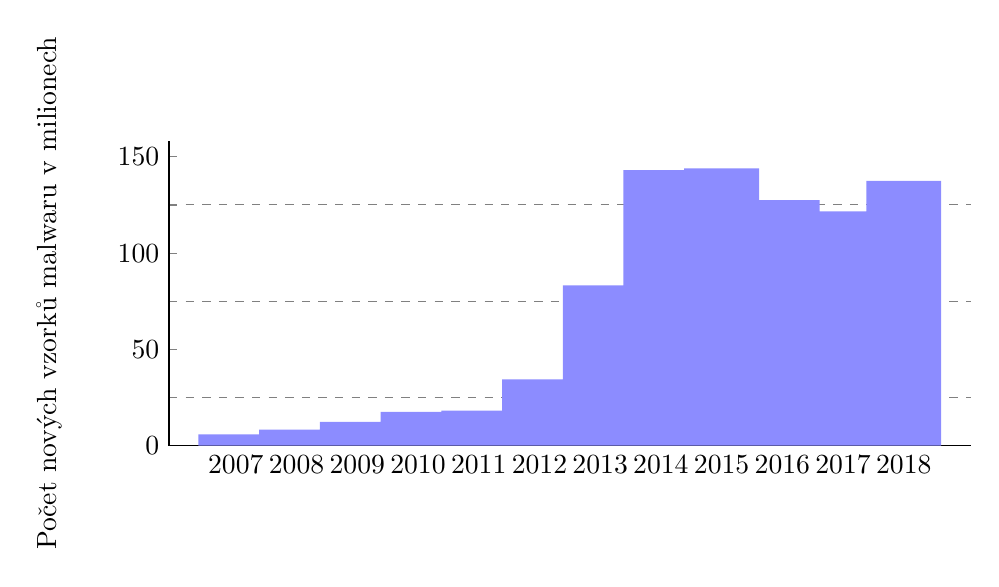
\begin{tikzpicture}
        \begin{axis}[
            ybar,
            bar width=.95cm, 
            width=.97\textwidth,
            height=.45\textwidth,
            ymajorgrids, 
            tick align=inside,
            major grid style={draw=white},
            axis x line*=bottom,
            axis y line*=left,
            ymin = 0,
            yminorgrids = true,
            y axis line style={opacity=100},
            tickwidth=0pt,
            enlarge x limits=true,
            legend style={
                at={(0.5,1)},
                anchor=north,
                /tikz/every even column/.append style={column sep=0.5cm}
            },
            grid=both,
            minor ytick={0, 25,...,150},
            ylabel={Počet nových vzorků malwaru v milionech},
            xtick=data,
            yticklabel style={text width=1cm,align=right},
            /pgf/number format/.cd,
                use comma,
                1000 sep={}
            ]
            nodes near coords={
                %\pgfmathprintnumber[precision=0]{\pgfplotspointmeta}
            }
        ]
        \addplot [draw=none, fill=blue!45] coordinates {
        	    (2007,5.9) 
        	    (2008,8.4)
        		(2009,12.4) 
        		(2010,17.6)
        		(2011,18.2)
        		(2012,34.4)
        		(2013,83.2)
        		(2014,143.1)
        		(2015,144.0)
        		(2016,127.5)
        		(2017,121.7)
        		(2018,137.5)
        	};
        \end{axis}
    \end{tikzpicture}
    
    \caption{Počet vzorků nového malwaru mezi roky 2007 - 2018. Zdroj dat \cite{av_securityreport_1819}}
    \label{fig:MalwareSamplesAV}
    
\end{figure}

Proto jsou vyvíjeny metody automatické analýzy (např. pomocí klasifikace výstupu analýzy kódu a jeho chování viz kapitola \ref{stateOfArt}), jež umožňují získat potřebná data o testovaných vzorcích včas a zmírnit tak případné dopady dosud neodhalené hrozby. Zároveň je také důležité, aby~daný poskytovatel anti-malwarových služeb měl zajištěn dostatečný přísun vzorků, které tvoří reprezentativní zástupce. Takto získané vzorky mohou tvořit databázi malwaru.

%Pro zajištění spolehlivosti testů jsou navrhovány ??
%Dále je také nezbytná spolehlivost analýzy. Proto jsou navrhovány nové postupy

Aby byl zohledněn vznik množství nových vzorků malwaru a také patřičná rychlost analýzy, je navrhováno množství nových přístupů a postupů při odhalování. 

U těchto postupů pak obecně rozlišujeme statickou a dynamickou analýzu, které jsou dále podrobně popsány v teoretické části.

Tato práce se bude dále zabývat především statickou analýzou, možnostmi jejího využití a~to~i~v~kombinaci s dalšími metodami, a jejími limity.

%nevýhody dynamické analýzy: potřeba virtuálního prostředí, které musí odpovídat reálnému (stejná verze operačního systému), 
%výhody statické analýzy: bez potřeby virtuálního prostředí, 

%% State of art
% 7 ruční analýza (popsané programy atd)
% 5 způsob převedení malwaru na obrazek a klasifikace
% 4 limity statické analzy
% 3 android malware analyza
% 2 klasifikace
% 1 staticka a dynamicka
%
% Analýza malware
\section{Analýza malwaru}

Analýza malwaru je proces při kterém se zkoumá chování vzorku. Předmětem takovéto analýzy je~zjistit, jak malware pracuje a jak jej případně eliminovat \cite{malwareanalysis_digitalguardian}. Výstup by měl obsahovat jednotlivé charakteristiky a funkcionality malwaru. Analýza podezřelých binárních souborů se~provádí v~bezpečném prostředí \cite{monnappaka2018}. Jak již bylo zmíněno, malware může nabývat mnoha podob jako například virus, červ, spyware nebo trojský kůň.

Analýza malwaru je prováděna v následujících případech \cite{malwareanalysis_digitalguardian}:

\begin{itemize}
    \item bezpečnostní incident v síti;
    \item za účelem zkoumání vzorku;
    \item indikace kompromitování systému.
\end{itemize}

Přístupy k analýze jsou dva a to pasivní a aktivní neboli statická a dynamická analýza. Popsány jsou v následujícím textu.

\subsection{Statická analýza}

Statická analýza je metoda, při níž není zkoumaný vzorek počítačového programu nebo jeho část spuštěn. Tento postup se využívá při analýze malwaru, testování aplikací, hledání zranitelnosti atd. Může se provádět buď ručně nebo pomocí specializovaného programu.

    Při statické analýze vzorku je nahlíženo na různé části programu jako jsou metadata, struktura souboru popřípadě zdrojový kód. 

%%Body k textu
%* bez spuštění
%* malware
%* testování aplikací / hledání zranitelností
%* možnosti:
%* * ručně
%* * automaticky
    %* hledání vzorů / signatur
    %* abstraktní interpretace
    %* vylepšení o neuronové sítě
    
% nastroje
% postupy
% metodika atd atd

%určení filetype (pe, elf..) (Y)
%vytvoření hashe (porovnání v db jestli už stejný soubor nemám)
%skenování antiviry - jestli už nějaká databáze neobsahuje
%extrakce stringu - ze souboru
%detekce packeru / obfuskace / komprese
%detaily spustitelného souboru (entry point atp) 
%klasifikace / širší analýza 

Průběh statické analýzy se může lišit případ od případu a nemusí být nutně provedeny všechny kroky \cite{monnappaka2018}. Obvykle však analýza malwaru začíná určením cílové platformy a to na základě informací získaných o spustitelném souboru a z něj. Například pokud podezřelý binární soubor v sobě obsahuje PE hlavičku, s velkou pravděpodobností se jedná o soubor určený pro operační systém Windows. 

%https://cs.qwe.wiki/wiki/List_of_file_signatures
Malware určený pro Windows často končí příponami .exe, .dll, sys. apod. Spoléhat se pouze na příponu však nelze. Útočník může použít nejrůznější způsoby jak příponu zakrýt tak, aby umožnil malwaru spuštění uživatelem. Proto by v kódu měla být použita signatura souboru, kterou známe také jako magická čísla\label{magic_numbers} \cite{magic_number}. Podpis souboru je totiž unikátní sekvence bytu v hlavičce souboru. Různé soubory mají různé signatury a lze je podle nich identifikovat \cite{file_signatures_2020}.

Dalším krokem je vytvoření unikátního otisku tzv. fingerprintu pomocí kontrolního součtu pro identifikaci daného vzorku a jeho porovnání s databází. Otisk souboru může být vytvořen pomocí libovolné hashovací funkce, která je používána v dané databázi. Aby bylo možné vzniklý otisk případně porovnávat s externími databázemi, je často vytvářeno více verzí pomocí více hashovací funkcí jako například MD5, SHA1 nebo SHA256. V případě, kdy by již vzorek existoval v databázi, není potřeba provádět další analýzu, protože její výsledek je již znám \cite{sikorski2012practical}.

Dále je pro zjištění zda má tento malware již známou signaturu případně fingerprint prováděn sken vícero anti-virovými programy \cite{sikorski2012practical}. Název signatury pak může sloužit k získání dalších informací o souboru a jeho vlastnostech. Pro tuto analýzu je možné použít například  nástroj VirusTotal, jenž obsahuje 7~desítek antivirů \cite{virustotal_howitworks}. 
    
Následuje extrakce obsažených řetězců (sekvence ASCII a UNICODE) obsažených v binárním souboru. Získání těchto obsažených řetězců může velmi usnadnit další analýzu podezřelého souboru. Například pokud se malware připojuje k CnC serveru, může obsahovat doménové jméno serveru, kde se CnC nachází. Dále mohou řetězce obsahovat například názvy souborů, které malware vytváří, URL adresy, IP adresy, informace o registrech atd. \cite{monnappaka2018}.

Protože je extrakce obsažených řetězců často klíčovým nástrojem jak získat informace o~malwaru a jeho funkcionalitě, snaží se proti ní útočnici svůj kód co nejvíce obrnit. A proto používají autoři škodlivého kódu packery (které provádí obfuskaci, šifrování a kompresi) tak, aby skryli malware před bezpečnostními experty. Tyto techniky totiž často velmi ztíží analýzu binárního souboru a oddálí tak detekci jejich malwaru.

Obsah hlavičky spustitelného souboru je dalším stěžejním bodem analýzy malwaru, obsahuje totiž důležité informace o zavedení do paměti a spuštění souboru, jeho struktuře, seznam potřebných knihoven atd. Tato analýza nám může například pomoci odhalit k čemu daný vzorek přistupuje (soubory, registry nebo třeba síť). Většina těchto operací je totiž prováděna pomocí API operačního systému a konkrétních knihoven. 

Následuje porovnání vzorku s jinými a jeho klasifikace. V případě malwaru jsou klasifikovány jednotlivé vzorky podle jejich charakteristik a podobností \cite{kaspersky_malware_classification}. Skupina, ve které se shlukují vzorky stejného typu, se nazývá rodina malwaru \cite{6107902}. 

Klasifikace do malwarových rodin je používána proto, že zatímco kontrolní součet souboru je skvělým nástrojem pro určení stejného vzorku, v případě malwaru se velmi často stává, že autor škodlivého kódu změní jen malou část kódu a tím změní celou hash \cite{monnappaka2018}.

\subsection{Dynamická analýza}
Narozdíl od statické analýzy je při dynamické analýze testovaný vzorek spuštěn. Vzorek se většinou testuje v kontrolovaném prostředí, v němž se vzorek spustí a sledují se změny, které provádí v systému. Vzhledem k tomu, že malware má uzavřený kód, je na něj při analýze nahlíženo jako na blackbox. Avšak většinou se při analýze malwaru kombinují obě techniky jak dynamická tak~statická analýza.

%%Body k textu
%* obdobně jako statická
%* program je spuštěn (musí být zkompilován / interpretován)
%* pak se sleduje jeho chování
%* vzhledem k tomu, že vetšinou má malware uzavřený kód, je na program nahlíženo jako blackbox
%* většinou se kombinují obě techniky

\section{Formát spustitelných souborů}
%https://en.wikipedia.org/wiki/Comparison_of_executable_file_formats
%https://dspace.vutbr.cz/xmlui/bitstream/handle/11012/53219/7141.pdf?sequence=1&isAllowed=y
%https://blog.malwarebytes.com/threat-analysis/2014/05/five-pe-analysis-tools-worth-looking-at/

%ABI vs API

% WHAT IS THIS AND HOW IT WORKS

%% Spustitelné soubory v operačních systémech
%%% srovnání atd

%% Obsah PE hlavičky

%%% WHAT IS THAT
%%% Analýza
%%% Aplikace

%%%%%
%%%%% CITACE
%%%%%

Spustitelný soubor je speciální druh souboru, který obsahuje instrukce pro provedení určité činnosti \cite{executable_lifewire}. Například se může jednat o strojový kód nebo zdrojový kód určený pro interpret. %Spustitelné soubory se oproti běžným souborům liší hlavně tím, že 

%Na rozdíl od běžných binárních (datových) souborů není spustitelné soubory 

Oproti běžným binárním souborům není v případě spustitelných souborů potřeba žádná externí aplikace k interpretovaní těchto dat. Aby bylo možné program spustit musí být formát souboru přizpůsoben operačnímu systému \cite{wiki:Executable}.

Ke spuštění programu dojde tak, že program zavaděče (anglicky loader), jež je běžně součástí operačního systému, načte program do paměti a připraví potřebné knihovny pro spuštění viz~obrázek č. \ref{fig:file_execution}.

\begin{figure}[!ht]
    \centering
    \caption{Proces spuštění souboru}
    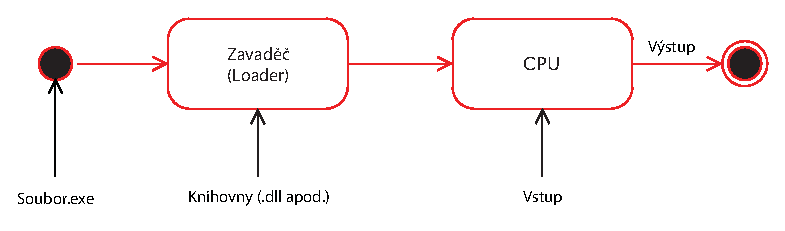
\includegraphics[width=150mm,scale=0.5]{Figures/obrazky/Execution.eps}
    \label{fig:file_execution}
\end{figure}

Aby ke spuštění mohlo vůbec dojít, musí operační systém podporovat formát spustitelného souboru na nízké úrovni  \cite{wiki:Executable}. K tomu slouží jasně definované rozhraní ABI (Application binary interface). Toto rozhraní definuje pravidla pro spolupráci strojového kódu a jádra OS. Podpora jednotného ABI na různých systémech pak umožňuje kompatibilitu zkompilované aplikace mezi různými systémy.

%https://en.wikipedia.org/wiki/Loader_(computing)
%https://en.wikipedia.org/wiki/Executable
%https://en.wikipedia.org/wiki/Application_binary_interface
%https://tristudy.com/flow-of-c-programming/

%https://cs.wikipedia.org/wiki/Zavad%C4%9B%C4%8D_(program)
%https://tristudy.com/flow-of-c-programming/

\subsection{Spustitelné soubory v OS}
% PE File, Elf, APK
%% V OS Windows PE File
%% V OS Linux ELF
%% Andorid APK

% Každý systém obsahuje jasně definované co obsahuje spustitelný soubor a 
% jaká je definovaná struktura
% v čem je rozdíl mezi systémy

%https://en.wikipedia.org/wiki/Comparison_of_executable_file_formats

Všechny operační systémy, které obsahují podporu zavedení vlastního programu, definují jeden nebo více podporovaných formátů spustitelných souborů. Tabulka č. \ref{table:executableFileformat} prezentuje některé spustitelné formáty a informace, na které platformě je můžeme najít.

%%%%% ROZDIL

\noindent
\begin{table}[H]
    \caption{Formáty spustitelných souborů (Zdroj dat \cite{wiki:Comparison_of_executable_file_formats})}
    \label{table:executableFileformat}
    
    \centering
    \begin{tabular}{|l|l|l|l|}
        \hline
        Formát & Platforma                               & 64-bit & Přípona     \\
        \hline
    	\hline
        PE     & \makecell[l]{Windows, ReactOS,\\ HX DOS Extender, BeOS} & Ne     &  .exe, .dll, .sys atd.  \\ \hline
        PE32+  & Windows & Ano    &  .exe, .dll, .sys atd.  \\ \hline
        NE     & \makecell[l]{MS-DOS, OS/2 Windows,\\ HX DOS Extender}   & Ne     &  .exe, .dll, .fon       \\ \hline
        ELF    & \makecell[l]{Unix-like, OpenVMS, BeOS,\\ Haiku}         & Ano    &  žádná, .bin, .o, .elf, .so atd.   \\ \hline
        Mach-O & \makecell[l]{NeXTSTEP, macOS, iOS,\\ watchOS, tvOS}     & Ano    &  žádná, .o, .dylib, .bundle  \\ \hline
    \end{tabular}
\end{table}

\subsection{PE hlavička}
\label{pe_format}
% Navržen pro Windows, stále obsahuje DOS hlavičku
% Obsahuje DOS hlavičku, aby DOS mohl rozpoznat, že se jedná o PE formát, a nemůže jej spustit
% Formát pro exáče, DLLtka atd,
% Hlavičky + sekce

%Tento formát byl navržen pro 
%PE hlavička je datová struktura, která obsahuje důležité informace pro zavaděč programu. 

%https://blog.kowalczyk.info/articles/pefileformat.html

Formát PE (zkr. Portable Executable) byl navržen jako nástupce předešlého formátu NE (zkr. New Executable) používaném v operačním systému MS-DOS. Tento nový formát byl poprvé uveden spolu s Windows NT. A je založen na UNIXové specifikaci COFF (zkr. Common Object File Format) \cite{pe_format_history}.

\paragraph*{Struktura souboru}

Hlavička spustitelného souboru obsahuje informace o spustitelném souboru (počet sekcí, velikost sekcí atp.) a sekce pak obsahují samotné části programu (kód programu, data atp.).

Jedná se o jasně definovanou strukturu určenou pro nativně spustitelné soubory EXE a DLL knihovny \cite{Zatloukal2017MalwareDB}. Tato struktura je složena ze dvou hlavních částí a to hlavičky a sekcí \cite{msdocs_pe}. Obrázek č. \ref{fig:peformat} prezentuje tuto strukturu.

\begin{figure}[!ht]
    \centering
    \caption{PE formát}
    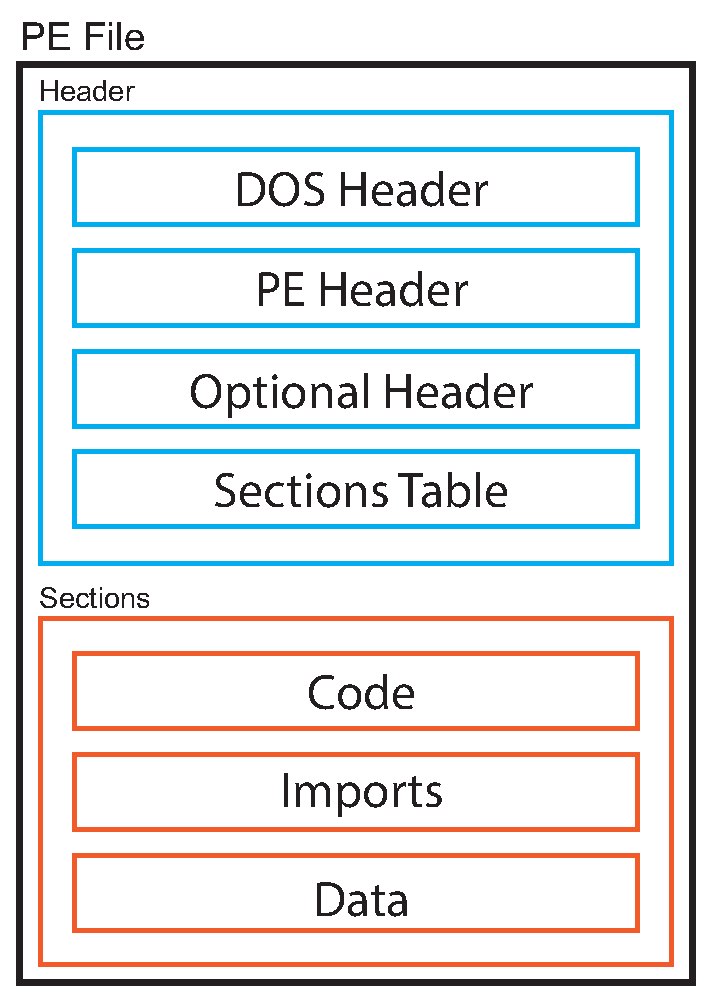
\includegraphics[width=60mm,scale=0.5]{Figures/obrazky/pe-file.eps}
    \label{fig:peformat}
\end{figure}


\paragraph*{Hlavička} Jak už bylo zmíněno, hlavička PE souboru obsahuje celou řadu důležitých metadat pro zavedení aplikace do uživatelského prostoru. Části této hlavičky jsou dále popsány v následujícím textu.

\subparagraph*{DOS Header}
%MSDOS hlavička + program pro dos CANNOT BE RUN IN DOS mode
Prvních 64 bytů souboru ve formátu PE vždy obsahuje program pro zajištění kompatibility s OS MS-DOS. Tento program slouží k upozornění, že se nejedná o aplikaci určenou pro prostředí MS-DOS. Po jeho spuštění se vypíše hláška \emph{This program cannot be run in DOS mode}. První hodnotou této DOS hlavičky je hodnota \emph{e\_magic} (magické číslo - viz \ref{magic_numbers}), které identifikuje DOS mód \cite{Zatloukal2017MalwareDB}. Zároveň tato hlavička obsahuje offset (logická adresa) \emph{e\_lfanew}, jež odkazuje na začátek PE hlavičky \cite{pe_format_history}.

\subparagraph*{PE Header} \ref{peheader_entrypoint}
Po DOS hlavičce následuje PE hlavička. Na offsetu 0x3C se nachází 4 bytový podpis identifikující soubor jako PE formát \cite{Liao2012PEHeaderBasedMS}. Tento podpis odpovídá hodnotě \emph{PE\textbackslash0\textbackslash0} \cite{msdocs_pe}.

\subparagraph*{Optional Header}
Následuje optional header (v překladu volitelná hlavička), která je však volitelná pouze v případě objektových souborů, kde by neměla význam a pouze by zabírala místo. Pro spustitelné EXE soubory a DLL knihovny je tato část povinná \cite{msdocs_pe}, obsahuje totiž důležité informace pro zavaděč jako například entry point (vstupní bod programu označovaný také jako~\emph{EP}) nebo počet sekcí \cite{pe_format_history}. 

\subparagraph*{Sections Table}

Po volitelné hlavičce následuje tabulka sekcí, jež obsahuje hlavičky jednotlivých sekcí spustitelného souboru. Každá hlavička obsahuje název sekce, její velikost, umístění a charakteristiky sekce \cite{infosecinstitute_pe}.

\paragraph*{Sekce}
%An application for Windows NT typically has the nine predefined sections named .text, .bss, .rdata, .data, .rsrc, .edata, .idata, .pdata, and .debug. Some applications do not need all of these sections, while others may define still more sections to suit their specific needs. 
Aplikace pro OS Windows mohou využít 9 předdefinovaných sekcí jako \emph{.text, .bss, .rdata, .data, .rsrc, .edata, .idata, .pdata a .debug} nebo si dle svých potřeb vytvořit vlastní \cite{pe_format_history}. 

Důležité sekce budou popsány níže.

\subparagraph*{Sekce .text}
Tato sekce obsahuje instrukce programu pro procesor, který je následně vykonává. Odkazuje na ni entry point v PE Header (viz \label{peheader_entrypoint}) Často je to jediná sekce, ze které je program spouštěn \cite{sikorski2012practical}.

\subparagraph*{Sekce zdrojových dat (.rsrc)}

Další sekcí je sekce \emph{.rsrc}. Tato sekce obsahuje zdroje (resources) pro běh programu, které nejsou uloženy přímo v programu. Jsou to například obrázky, binární data nebo řetězce, které však mohou být přímo součástí kódu. Tyto sekce jsou často využity kupříkladu v programech, které obsahují více jazykových mutací \cite{sikorski2012practical}.

\subparagraph*{Datové sekce (.bss, .rdata, .data)}

Po sekci zdrojových dat následují sekce datové. Sekce \emph{.bss} (Block Started by Symbol) obsahuje neinicializovaná data aplikace jako statické proměnné apod. V další sekci \emph{.rdata} jsou uložena data určená pouze pro čtení jako globální konstanty atd. \cite{infosecinstitute_pe}. Poslední typ datové sekce je pak sekce \emph{.data}, jež obsahuje globální data, která jsou přístupná z jakékoliv části kódu v aplikaci. \cite{sikorski2012practical}

\subparagraph*{Sekce s exporty (.edata)}

Sekce \emph{.edata} obsahuje informace k exportům jako názvy a~adresy exportovaných funkcí \cite{infosecinstitute_pe}.

\subparagraph*{Sekce s importy (.idata)}

Po sekci s exporty je nutno také zmínit sekci \emph{.idata}, která~naopak obsahuje informace k importům (adresní tabulka importu aj.) \cite{infosecinstitute_pe}. 

%\subparagraph*{Sekce  (.tls)}
%Poslední důležitou sekcí je \emph{.tls} sekce, jež obsahuje

\paragraph*{Nástroje pro analýzu}

Nástrojů pro analýzu spustitelných souborů existuje celá řada. V~následujícím textu budou zmíněny některé z nich. 

\subparagraph*{PEiD}
% detekce packeru, kryptoru, komprese
% vyvoj ukončen 
% pouze PE
% detekce signatur možnost dodat svoje
% https://ieeexplore.ieee.org/abstract/document/4654055 \cite{4654055}

Tento nástroj je jeden z nejpoužívanějších. Je určen pro detekci známých packerů, kryptorů a kompilátorů na základě databáze signatur. V základu obsahuje databázi více než 470 signatur, je však možné přidat i své vlastní. Existují také databáze obsahující přes 3000 signatur, které je možné použít s aplikací PEiD. Detekce pomocí PEiD je ve srovnání s jinými aplikacemi pro detekci packerů velmi dobrá. Obsahuje také rozhraní připravené pro další rozšíření \cite{4654055}. 

Na následujícím obrázku č. \ref{fig:peid} je možné vidět prostředí aplikace PEiD. První část obsahuje základní informace exportované z PE hlavičky jako například, v jaké sekci se nachází entry point nebo jeho offset. Ve spodní části pak lze vidět použitý detekovaný kompilátor nebo packer (viz kapitola \ref{packers}). V našem případě byl detekován packer UPX.

\begin{figure}[!ht]
    \centering
    \caption{Program PEiD}
    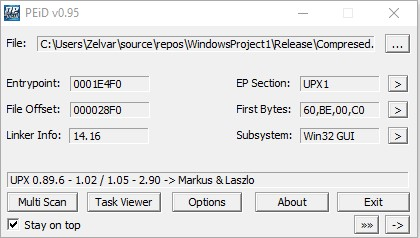
\includegraphics[width=100mm,scale=0.5]{Figures/obrazky/PEid.jpg}
    \label{fig:peid}
\end{figure}

Pod základním výstupem pak nástroj nabízí různé možnosti nastavení jako například přepnutí úrovně skenování. Nabízené možnosti skenování jsou \emph{Normal mode}, který vyhledává signatury okolo EP, \emph{Deep mode} skenuje celou sekci. \emph{Deep mód} detekuje až 80\% souborů, které jsou chráněny před analýzou pomocí packerů. Poslední možností je \emph{Hardcore mode}, který skenuje celý PE soubor na známé signatury \cite{peid_info} což však může trvat výrazně delší dobu.

Nevýhodou tohoto nástroje je, že neumí pracovat s aplikacemi určenými pro platformu x64 (PE32+). Další vývoj již neprobíhá.

\subparagraph*{Exeinfo PE}

Alternativou PEiD může být nástroj Exeinfo, který podporuje také PE32+. Hlavní výhodou je, že vývoj programu stále probíhá (poslední verze vyšla 22.10.2019) \cite{exeinfo}. 

Uživatelské rozhraní je velmi podobné PEiD (viz obrázek č. \ref{fig:exeinfo}), výstup také obsahuje nápovědu s~návodem k~provedení unpackingu (viz kapitola \ref{unpackers}).

Nevýhodou však je to, že program neumí detekovat starší způsoby ochrany (např. packery nebo protektory viz kapitola \ref{packers}) \cite{exeinfo_malwarebytes}.

\begin{figure}[!ht]
    \centering
    \caption{Program Exeinfo PE}
    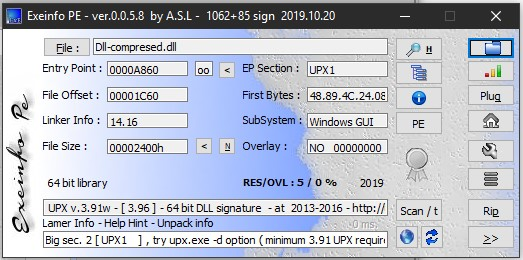
\includegraphics[width=100mm,scale=0.5]{Figures/obrazky/Exeinfo.jpg}
    \label{fig:exeinfo}
\end{figure}


\subparagraph*{PE Studio}

Dalším možným nástrojem pro práci se spustitelným souborem formátu PE je PE Studio. Tento program je nabízen ve dvou variantách, jedna je zdarma a nabízí základní statickou analýzu souboru, a druhá pokročilá je nabízena za poplatek \cite{pestudio}. Na obrázku č. \ref{fig:pestudio} je možné vidět rozhraní tohoto programu (konkrétně jeho bezplatné verze).

Základní verze programu obsahuje běžně nabízené funkce konkurenčními aplikacemi mimo jiné ale také pokročilejší funkce, které nazývá indikátory. Tyto indikátory využívají metody jako je detekce signatur, detekce URL a IP adres v~kódu, vyhledávaní zakázaných řetězců ze slovníku (keyloger apod.), hledání klíčových slov mezi řetězci atp. \cite{exeinfo_malwarebytes}.

Výstup programu je rozdělen chronologicky do několika podoken (viz obrázek č. \ref{fig:pestudio}) dle funkcí. Obsahuje jak již zmíněné indikátory, tak výstup z nástroje VirusTotal, seznam řetězců, seznam sekcí atd.

\begin{figure}[!ht]
    \centering
    \caption{Nástroj PE Studio}
    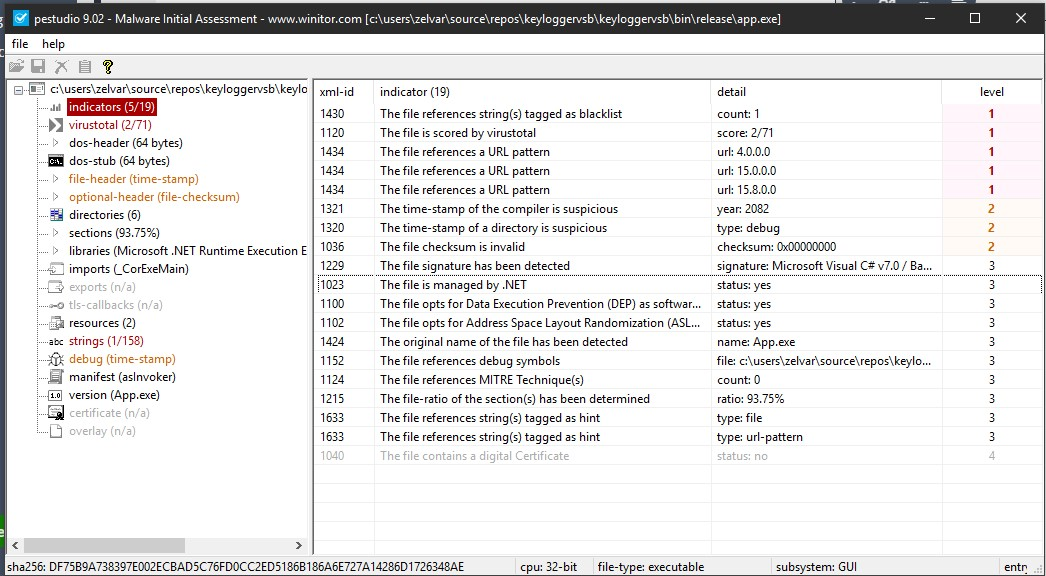
\includegraphics[width=160mm,scale=1]{Figures/obrazky/PeStudio.jpg}
    \label{fig:pestudio}
\end{figure}
\section{Základní nástroje statické analýzy}

\subsection{Debugger}
%% http://programujte.com/clanek/2006080803-cracking-2-cast/

Debugger je nástroj, který slouží primárně k ladění softwaru. Zároveň je ale také velmi důležitým nástrojem, pokud je potřeba zjistit, jak program pracuje. Umožňuje totiž krokovat kód instrukci po instrukci (v~případě interpretovaného kódu pak řádek po řádku) a zároveň sledovat změny hodnot v registrech, zásobníku nebo paměti.

Další důležitou funkcí debuggeru jsou breakpointy \cite{debugger_dissasembler}. Breakpoint lze nastavit kdekoliv v~kódu a jakmile na něj program narazí, vyvolá přerušeni. Je možné tedy například zjistit stav zásobníku v každém kroku smyčky.

Debuggerů existuje celá řada. Velmi populárním je například OllyDbg viz obrázek č. \ref{fig:olldbg}. Tento debugger umožňuje všechny potřebné funkce pro sledování registru, volání API, konstant, stringu atd. Má přívětivé uživatelské prostředí a lze do něj vložit externí rozšíření \cite{ollydbg}. Bohužel s ním lze debuggovat pouze 32-bitové aplikace.

\begin{figure}[!ht]
    \centering
    \caption{Debugger OllyDbg}
    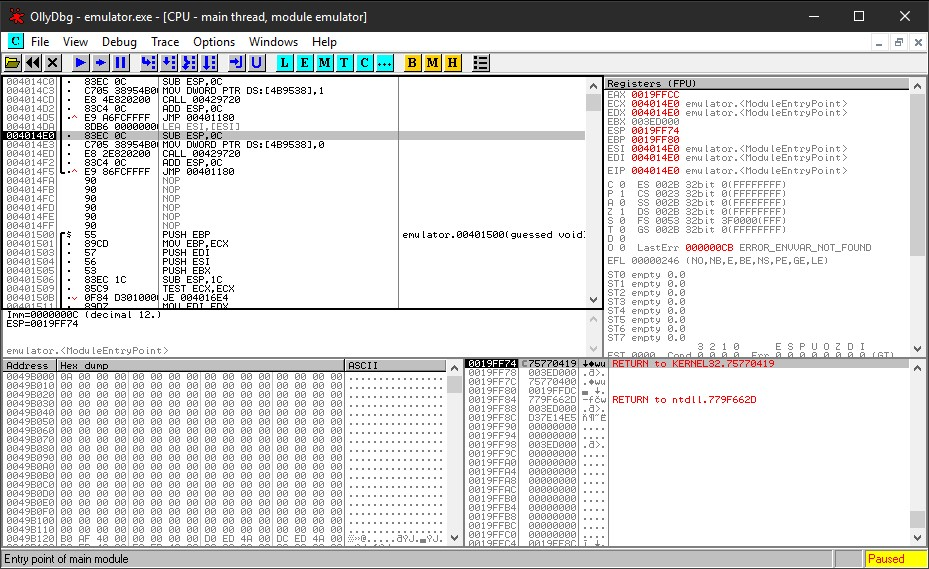
\includegraphics[width=140mm,scale=0.5]{Figures/obrazky/OllyDbg.jpg}
    \label{fig:olldbg}
\end{figure}

\subsection{Disassembler}
%what is that and how it works
%https://reverseengineering.stackexchange.com/questions/11466/how-does-disassembler-really-work

Disassembler umožňuje převod kódu zpět do programovacího jazyka nejčastěji assembleru \cite{debugger_dissasembler}. Existují také pokročilejší disassemblery, které umí převést strojový kód do C nebo jiného jazyka. Kvalita takovýchto převodů není valná (nezískáme původní zdrojový kód) a je vhodná spíše pro lepší orientaci v konstrukcích programu. Oproti debuggeru nelze dissasembleru v jeho procesu nijak zabránit. Proto však jsou využívány další techniky ochrany před analýzou jako obfuskace, komprese nebo šifrování.

%\paragraph*{Metoda lineárního průchodu}
%\paragraph*{Analýza rekurzivním sestupem}

\subsection{HEX editor}

HEX editor slouží ke zkoumání a editaci na úrovni bytů a bitů. Nejčastěji se souborem pracuje v šestnáctkové soustavě, proto tedy HEX editor. Některé editory také umožňuji zobrazit data jako ASCII nebo Unicode, hledat určité vzory apod. Existuje spousta HEX editorů. Vhodným  může být například \emph{FileInsight}, jehož autorem je společnost McAfee Labs. Tento editor je zachycen na obrázku č. \ref{fig:hexeditor}. Tento HEX editor zvládne kromě běžných funkcí, jako je například editace binárních dat, také zobrazit strukturu PE souboru, dissasemblovat 32-bitové aplikace nebo dekódovat některé metody obfuskace (XOR, posun, Base64) \cite{hexeditors}.

\begin{figure}[!ht]
    \centering
    \caption{HEX editor FileInsight}
    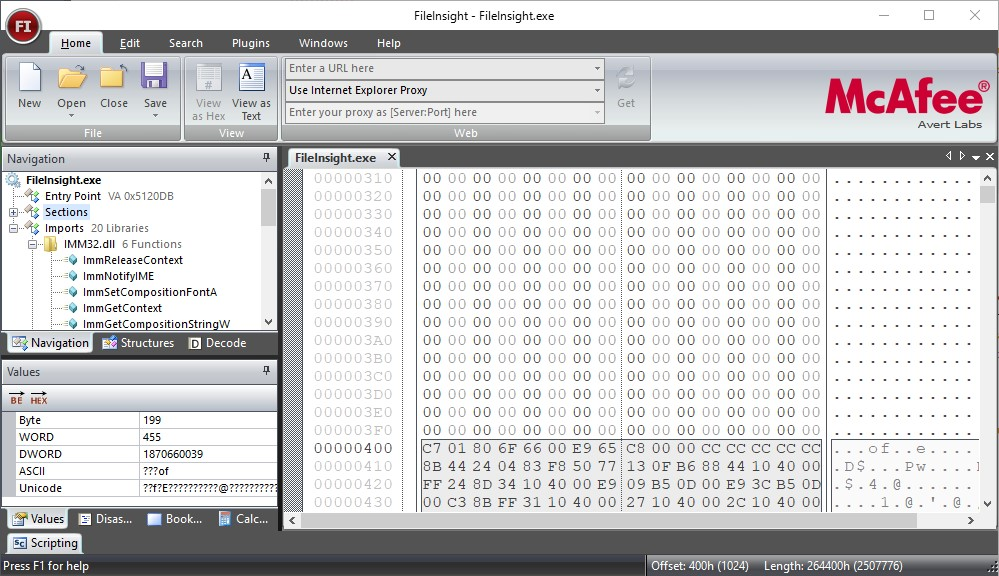
\includegraphics[width=150mm,scale=0.5]{Figures/obrazky/MCAfee-Insights.jpg}
    \label{fig:hexeditor}
\end{figure}

\subsection{Balík sysinternals}
%https://www.chip.cz/casopis-chip/01-2017/windows-sysinternals/
%https://docs.microsoft.com/en-us/sysinternals/

Balík programů sysinternals obsahuje nespočet utilit, které umožňují rozšířit základní funkce Windows \cite{chip_sysinternals}. Kolekce obsahuje například nástroje pro zjištění informací o systému, detailní správce běžících procesů apod. Tato sada je dostupná zdarma a lze stáhnout ze stránek Microsoftu.

Pro analýzu malwaru můžeme z této sady použít například aplikaci \emph{Strings} \cite{ms_sysinternals}, která slouží k extrakci obsažených řetězců v požadovaném souboru. V případě dynamické analýzy by bylo možné použít například \emph{Process Explorer}.

\subsection{Dependency Walker}
Tento nástroj slouží k analýze závislosti zkoumaného souboru. Umožňuje analyzovat různé moduly Windows (jako .exe, .dll, .ocx, .sys atd.) \cite{depedencywalker}. A to jak 32 bitové, tak 64 bitové. Následně jsou vazby zobrazeny programem v hierarchické stromové struktuře viz obrázek č. \ref{fig:depedency}. Dalším výstupem je seznam potřebných souborů včetně detailních informací o plné cestě k souboru atd.

\begin{figure}[!ht]
    \centering
    \caption{Dependency Walker}
    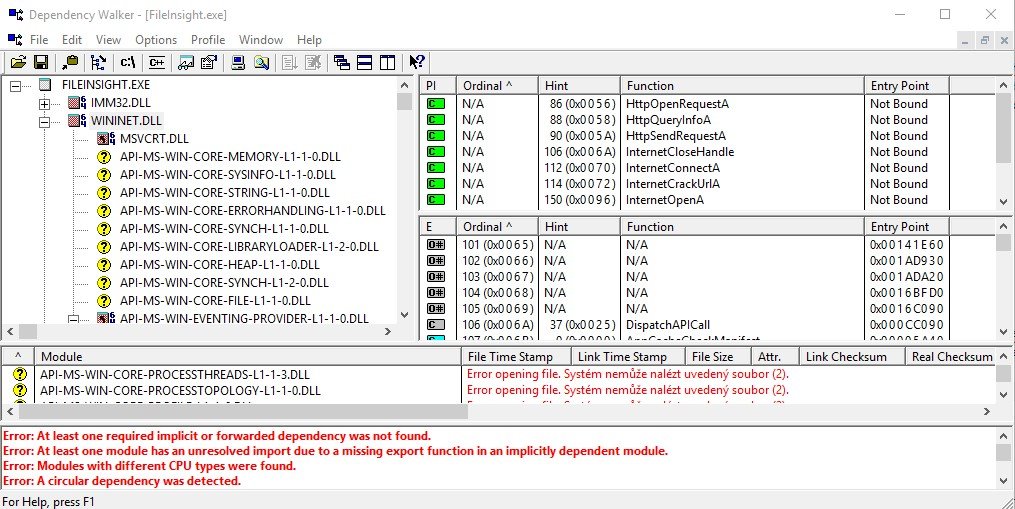
\includegraphics[width=150mm,scale=0.5]{Figures/obrazky/DependencyWalker.jpg}
    \label{fig:depedency}
\end{figure}

\section{Obranné mechanismy proti analýze softwaru}

Postupy obrany proti analýze využívá jak běžně užívaný software pro účel ochrany duševního vlastnictví, tak i škodlivý kód k znesnadnění odhalení. Tato ochrana počítačových programů může být provedena více způsoby. Těmito způsoby se dále zabývá tato kapitola.

%%% MALWARE
%%% Ochrana programu proti crackování atd
%%% DRM

\paragraph*{Ochrana duševního vlastnictví}
Vlastníci práv a autoři softwaru využívají různé techniky, kterými se snaží ochránit své duševní vlastnictví například algoritmy (komunikační protokol programu Skype). Často se však také jedná o multimediální obsah, který obsahuje nějakou ochranu. Příkladem mohou být počítačové hry, u kterých se vydavatelé snaží ochránit hru před tzv. crackingem, kdy se nejrůznější organizace snaží prolomit a odstranit ochranu hry. 

%% Multimediální obsah, snaží se ochranit software, filmy, hudbu aby nebylo možné jednoduše prolomit ochranu k sw
%% Skrytí myšlenek před konkurencí - Skype
%% DRM ochrana médií
%% https://en.wikipedia.org/wiki/Denuvo - odolavalo fest dlouho

\paragraph*{Malware}

Autoři malwaru se stále snaží vymýšlet nové techniky ukrytí malwaru a znemožnění nebo alespoň ztížení jeho analýzy. 
%% chcou být o krok napřed
%% neodhalitelní

\subsection{Anti-debug}
\label{anti_debug}

Tento způsob ochrany brání ladění neboli debugovaní programu. Implementují ho často jak~legitimní aplikace, které potřebuji utajit své know-how, tak i tvůrci malwaru. Existuje mnoho způsobů jak přítomnost debuggeru detekovat a případně ho blokovat. Mezi ty nejpopulárnější patří následující \cite{sikorski2012practical}.

\paragraph*{Windows API}

Microsoft Windows obsahuje ve svém API několik zpusobů jak debugger detekovat. Některé funkce byly navrženy přímo pro detekci debuggeru, některé zase pro jiné účely, ale lze je pro detekci použít.

Nejjednodušším způsobem je použít metodu \emph{IsDebuggerPresent}. Tato metoda sleduje strukturu PEB, která obsahuje informace o aktuálním procesu, včetně pole \emph{IsDebugged}. Pokud je~toto pole nastaveno na nulu, debugger není přítomen. V opačném případě je program spuštěn v~debug režimu.

Obdobným způsobem můžeme použít metodu \emph{CheckRemoteDebuggerPresent}, která funguje na podobném principu. Rozdíl spočívá v tom, že tato funkce byla navržena ke sledování debuggu cizího (vzdáleného) procesu. Lze ji však nastavit tak, aby plnila i tento úkol.

Další možností je funkce \emph{NtQueryInformationProcess}. Metoda opět slouží k získání informací o požadovaném procesu. Prvním parametrem funkce je ukazatel na proces. Dalším parametrem je pak možné nastavit typ získané informace. 

Alternativním řešením bez sledování struktury PEB může být \emph{OutputDebugString}. Funkce slouží k odeslání řetězce na výstup debuggeru. Pokud však debugger nebude přítomen a chybový kód bude nastaven pomocí funkce \emph{SetLastError} bude po zavolání \emph{OutputDebugString} na výstupu chybový kód funkce \emph{OutputDebugString}. V případě, že by debugger přítomen byl, na výstupu bude chybový kód, který byl nastaven přes funkci \emph{SetLastError}.

\paragraph*{Detekce chování debuggeru}

Další variantou této ochrany je detekce základní funkce debuggeru a to breakpointu \cite{deepinstrinct_antidebug}. Breakpoint slouží analytikovi k zastavení kódu a funguje na principu vložení instrukce \emph{INT 3} do kódu. Instrukce \emph{INT 3} slouží k vyvolání breakpointu neboli přerušení. Malware však může skenovat sám sebe a hledat tuto instrukci v kódu. Případně vytvářet za~běhu kontrolní součet nebo hash aby zjistil, zda nebylo zasaženo do kódu.


\paragraph*{TLS callback}
%https://www.deepinstinct.com/2017/12/27/common-anti-debugging-techniques-in-the-malware-landscape/
%https://docs.microsoft.com/cs-cz/cpp/parallel/thread-local-storage-tls?view=vs-2019
TLS je místní paměťový prostor v rámci jednoho vlákna, kde může dané vlákno ukládat svá data \cite{msdocs_tls}. Tato vlastnost může být zneužita tak, že ještě před vstupním bodem programu, kdy je inicializováno vlákno aplikace, se zavolá potřebná funkce \cite{deepinstrinct_antidebug}.


\paragraph*{Zneužití zranitelnosti debuggeru}
%https://exchange.xforce.ibmcloud.com/vulnerabilities/16711
Stejně jako každý software i debuggery mohou obsahovat zranitelnosti. Autoři malwaru si to samozřejmě uvědomují a této skutečnosti zneužívají. Příkladem může být chyba známého a používaného debuggeru OllyDbg ve verzi 1.1 \cite{CVE-2004-0733}, která umožňovala aplikaci shodit pomocí formátovacího řetězce, zaslaného přes Windows API metodou \emph{OutputDebugString}.
\subsection{Obfuskace}
%https://researchspace.auckland.ac.nz/bitstream/handle/2292/3491/TR148.pdf
%https://searchsoftwarequality.techtarget.com/definition/obfuscation
%https://securityintelligence.com/an-example-of-common-string-and-payload-obfuscation-techniques-in-malware/
\label{obfuskacni_metody}

Obfuskace je transformace kódu takovým způsobem, aby bylo zamezeno či alespoň znesnadněno analyzování daného kódu člověkem, přičemž funkčnost kódu setrvává \cite{13355040520180901} \cite{Obfuscation}. Je možno využít různé techniky. Tyto techniky mohou být například: 

\paragraph*{Obfuskace struktury}
Tato transformace se řadí mezi ty nejjednoduší. Mění strukturu zdrojového kódu programu. Přeměna je jednosměrná a již nelze získat původní zdrojový kód. Při~této obfuskaci jsou odstraněny komentáře, mění se formátování (např. minifikací - odstranění nepotřebných znaků ze zdrojového kódu), je provedena změna názvů metod ( metoda() = \_a()) a proměnných ( string heslo = string a ).

%% transformace mění strukturu programu
%% jsou odstraněny komentáře v kódu
%% mění se formátování, název metod/funkcí ( funkce() = _a() ) / proměnných ( heslo = a )
%% jednosměrné , nelze získat původní kód
\paragraph*{Datová obfuskace}
%https://researchspace.auckland.ac.nz/bitstream/handle/2292/3491/TR148.pdf¨
%https://www.paladion.net/blogs/code-obfuscation-part-2-obfuscating-data-structures
%https://medium.com/better-programming/code-obfuscation-introduction-to-code-obfuscation-part-1-93a6797349b0
%https://selab.fbk.eu/ceccato/papers/2015/spro2015.pdf

Metoda datové obfuskace pracuje s maskováním datových struktur pomocí jejich přeměny na jiné sémanticky však stejné. Tento druh obfuskace se často používá pro skrytí citlivých informací. V případě malwaru se může jednat o důležité informace jako například doménové jméno či IP adresy CnC serveru, šifrovací klíče apod. Tyto transformace mohou být provedeny několika způsoby a jsou popsány níže \cite{DataObfuscation}.

\subparagraph*{Nahrazení statických dat}
%% Změna datových struktur
%% převod proměnných na metody
%% globalizace

Nejjednodušší způsob obfuskace statických dat je nahrazení metodou. Data jsou nahrazena kódem, který je bude dynamicky generovat. Účinnost tohoto řešení se zvyšuje s počtem volaných funkcí, jejichž volání je náhodně rozloženo do toku programu \cite{DataObfuscation}. Pro zmatení reverzního inženýra je možné přidat také několik výstupů, ke kterým při~normálním běhu programu nedojde.

Tuto metodu lze vidět na následující ukázce č. \ref{src:StaticData}. Statická data byla nahrazena jednoduchým \emph{switchem}, který podle čísla vstupu vrátí požadovanou hodnotu.

\noindent
\begin{minipage}[t]{1\textwidth}
    \lstinputlisting[basicstyle=\footnotesize,caption={Generování statických dat},label=src:StaticData]{zdrojaky/obfuskace/staticka-data.cs}
\end{minipage}

\subparagraph*{Rozdělení proměnných}
%% Změna z a=123 na a = 100 ; b = 20; c = 3 ; a + b + c 

Velmi účinnou technikou obfuskace proměnných je jejich rozdělení a to nejlépe za použití různých datových typů \cite{DataObfuscation2}. Cílem je zmást reverzního inženýra velkým množstvím použitých proměnných. \par Síla a odolnost této transformace roste s počtem použitých proměnných a různorodosti jejich typů.

Následující ukázka kódu č. \ref{src:VariableJoining1} a \ref{src:VariableJoining2} prezentuje tuto metodu. Původní proměnnou je možné vidět v prvním výpisu č. \ref{src:VariableJoining1} obfuskvanou proměnnou pak v ukázce č. \ref{src:VariableJoining2}. Pokud bychom definice proměnných proložili sekvencemi vykonávaného kódu docílili bychom ještě lepšího výsledku.

%\ref{ref:SkladaniPromenne}

%%%%%%%%%%%%%%% Výstup %%%%%%%%%%%%%
%\begin{center}	
    %\label{src:SkladaniPromenne}
    \noindent
    \begin{minipage}[t]{1\textwidth}
        \noindent
        \centering
        \lstinputlisting[basicstyle=\footnotesize,caption={Proměnná bez obfuskace},label=src:VariableJoining1]{zdrojaky/obfuskace/skladani-promenne1.cs}
    \end{minipage}
    \newline
    %\hfill
    \begin{minipage}[t]{1\textwidth}
        \lstinputlisting[basicstyle=\footnotesize,caption={Obfuskovaná proměnná},label=src:VariableJoining2]{zdrojaky/obfuskace/skladani-promenne2.cs}
    \end{minipage}
%\end{center}
%%%%%%%%%%%%%%%%%%%%%%%%%%%%%%%%%%%%%%


\subparagraph*{Globalizace proměnné}
%%% TODO
Máme-li funkce, například FA() a FB(), jež používají stejnou lokální proměnnou, definovanou ve svém těle a nevykonávají-li se souběžně, můžeme takovouto proměnnou deklarovat globálně a bude tak sdílena mezi oběma funkcemi \cite{DataObfuscation}. 

\subparagraph*{Sloučení proměnných}
%% sloučení více proměnných do jedné třeba 2 32b čísla mohou být jako 64b

Další metodou obfuskace proměnných je jejich sloučení do jedné. Příkladem mohou být dvě 32-bitová čísla X a Y. Tato čísla mohou být sloučena do jednoho 64-bitového dle následujícího vzorce \ref{src:SlouceniPromennychDo64b} \cite{DataObfuscation}.

\begin{equation}
    \label{src:SlouceniPromennychDo64b}
    V = 2^{32} * Y + X
\end{equation}

Odolnost této přeměny je malá, protože deobfuskátor může odhadnout, že proměnná~V se skládá ze dvou proměnných a to zkoumáním aritmetických operací.


\subparagraph*{Šifrování a kódování}
%% TODO
%% Zašifruji data
%%https://medium.com/@bromiley/malware-monday-obfuscation-f65239146db0

Další možností obfuskace dat je jejich šifrování popřípadě jejich kódování. Šifrovány mohou být buď jednotlivé části kódu nebo celé sekce spustitelného souboru \cite{sevagas_2014}. Zašifrovaná data jsou následně při spuštění dešifrována \cite{guardsquare_2019}. Tím je zaručeno, že program funguje tak jak byl vytvořen.

Často je možné se setkat s šifrováním pomocí bitové funkce \emph{XOR} nebo kódováním do \emph{Base64}. Takovéto zakrytí dat může oddálit odhalení skutečného obsahu, protože nemusí být na první pohled patrné, že jsou data šifrována nebo kódována.


%Oproti šifrování, užívaném například v síťové komunikaci, se používají také často již prolomené šifry. 
%Můžeme se setkat s šifrováním pomocí bitové funkce XOR nebo kódovaní do Base64. Takovéto zakrytí dat může prodloužit odhalení skutečného obsahu, protože při spuštění se kód prvně dešifruje a 

        %http://www.hjp.at/doc/rfc/rfc4648.html#sec_4
        %https://iopscience.iop.org/article/10.1088/1742-6596/1007/1/012003/pdf
        
        
Kódování \emph{Base64} bylo původně navrženo pro přenos příloh v emailové komunikaci a je~součásti standardu MIME \cite{sikorski2012practical}. Kódování \emph{Base64} umožňuje převést binární data na ASCII řetězec~a, jak~značí číslo 64 v názvu kódování, používá se právě 64 (resp. 65) znaků US-ASCII. Znaky užívané kódováním jsou a-z, A-Z, 0-9, +, / a = pro zarovnání délky \cite{RFC4648}.

Implementace do vlastního programu je velmi jednoduchá a většina moderních programovacích jazyků už toto kódování umožňuje. Útočnici (autoři malwaru) tak často využívají toto kódování ke skrytí závadného kódu nebo dat. 

%check this:
%Kódování pomocí Base64 umožňuje převést binární data na ASCII řetězec. Tím pádem lze přenést binární data jakoukoliv cestou. Původně bylo navrženo pro přenos příloh v emailové komunikaci. 

% komplikuje to zjištění co je obsahem
% umožňuje použít vlastní abecedu
% má popsaný algoritmus přesně (RFC)
% 

Šifrování pomocí exkluzivní disjunkce (\emph{XOR}) je velmi oblíbeným způsobem šifrováním mezi tvůrci malwaru \cite{sikorski2012practical}, protože se jedná o oboustrannou funkci, není potřeba implementovat různé algoritmy pro šifrování a dešifrování \ref{fig:XorSifrovani}. Klíčem je vždy proud bitů \cite{kpb_ochodkova2019}.

\begin{figure}[!ht]
    \caption{De/šifrování pomocí XOR}
    \centering
    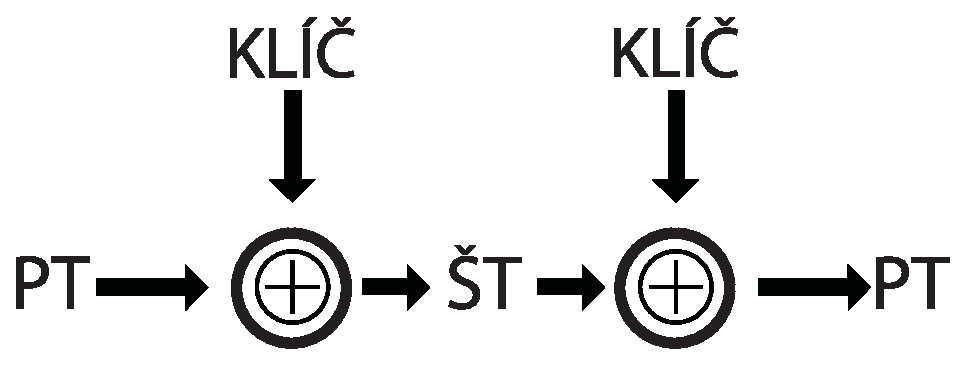
\includegraphics[width=75mm,scale=0.5]{Figures/obrazky/pt-st-pt-xorsifra.eps}
    \label{fig:XorSifrovani}
\end{figure}
    
%Šifrování pomocí exkluzivní disjunkce je velmi jednoduché na implementaci a protože se jedná o oboustrannou funkci, odpadá nutnost impl. Klíčem je vždy proud bitů. 
 
 
 
 % oboustranná funkce P -> C -> P
\paragraph*{Obfuskace běhu programu}
Tato transformace je využívána za účelem maskování posloupnosti kódu. Provádí se například záměnou pořadí prováděných instrukcí pomocí podmíněných skoků, vloženým nahodilým mrtvým kódem atd. \cite{13355040520180901}.
%https://www.paladion.net/blogs/code-obfuscation-part-3-hiding-control-flows

%%%%%%%%%%%%%%%%%%%%%%%%%%%%%%%%%%%%%%

\subparagraph*{Změna pořadí prováděného kódu}
Tento typ obfuskace spočívá v tom, že jsou provedeny skoky mezi jednotlivými částmi programu, které jsou náhodně rozmístěny. Přestože probíhají skoky, chování počítačového programu se nezmění. Tato metoda je v podstatě jednoduchá nicméně v delším kódu komplikuje analýzu pořadí prováděných operací \cite{13355040520180901}. 

Princip prezentuje následující výstup kódu č. \ref{src:ChangedOrder1} a \ref{src:ChangedOrder2}. Kód byl rozdělen do několika části (\emph{.start, .end a .continue}) následně byl náhodně rozmísten. Podmíněné skoky (\emph{JMP}) pak zajistí aby došlo k vykonání kódu ve správném pořadí.

%%%%%%%%%%%%%%% Výstup %%%%%%%%%%%%%
\noindent
\begin{minipage}[t]{.475\textwidth}
    \lstinputlisting[basicstyle=\footnotesize,label=src:ChangedOrder1,caption={Původní kód funkce bez obfuskace}]{zdrojaky/obfuskace/zmena-poradi-kodu1.asm}
\end{minipage}
\hfill
\begin{minipage}[t]{.475\textwidth}
    \lstinputlisting[basicstyle=\footnotesize,label=src:ChangedOrder2,caption={Obfuskovaný kód funkce}]{zdrojaky/obfuskace/zmena-poradi-kodu2.asm}
\end{minipage}
%%%%%%%%%%%%%%%%%%%%%%%%%%%%%%%%%%%%%%

\subparagraph*{Vložení nahodilého kódu}
Tato technika obfuskace je založena na vložení mrtvého nebo nepodstatného kódu do programu. Využívají ji především útočnici, protože pomocí této metody lze vytvořit novou verzi programu, která se chová stejně. Účel spočívá především ve zmatení detekce antiviry, protože vložený kód změní signaturu programu (známé signatury jsou využívány pro rychlou detekci malwaru) \cite{13355040520180901}. 

Ukázka následujících výpisu č. \ref{src:RandomCodeInserted1} a \ref{src:RandomCodeInserted2} prezentuje rozdíl hlavně v délce kódu. Do kódu bylo vloženo několik skoků pomocí \emph{JMP} a instrukcí \emph{NOP}, která nevykonává žádnou operaci.

%%%%%%%%%%%%%%% Výstup %%%%%%%%%%%%%
\noindent
\begin{minipage}[t]{.475\textwidth}
    \lstinputlisting[basicstyle=\footnotesize,label=src:RandomCodeInserted1,caption={Původní kód bez obfuskace vloženého kódu}]{zdrojaky/obfuskace/vlozeni-nahodileho-kodu1.asm}
\end{minipage}
\hfill
\begin{minipage}[t]{.475\textwidth}
    \lstinputlisting[basicstyle=\footnotesize,label=src:RandomCodeInserted2,caption={Kód funkce po obfuskaci}]{zdrojaky/obfuskace/vlozeni-nahodileho-kodu2.asm}
\end{minipage}
%%%%%%%%%%%%%%%%%%%%%%%%%%%%%%%%%%%%%%

\subparagraph*{Nahrazení ekvivalentem}
Díky nahrazení části kódu ekvivalentem lze provádět stejnou funkcionalitu programu různými způsoby. Tím je možné dosáhnout změny signatury, což způsobí vyšší náročnost detekce malwaru, takto vznikají nové verze u nichž je potřeba uchovat signaturu každé nové jedinečné verze \cite{13355040520180901}. 

Následující výpisy kódu č. \ref{src:ReplacedByEkvivalent1} a \ref{src:ReplacedByEkvivalent2} prezentují tuto metodu. Kód se liší ve dvou podstatných instrukcích, jež vykonávají ekvivalentní funkci a to instrukce \emph{test} nahrazena ekvivalentem \emph{cmp} a instrukce \emph{inc} nahrazena \emph{add}.

%%%%%%%%%%%%%%% Výstup %%%%%%%%%%%%%
\noindent
\begin{minipage}[t]{.475\textwidth}
    \lstinputlisting[basicstyle=\footnotesize,label=src:ReplacedByEkvivalent1,caption={Kód před nahrazením}]{zdrojaky/obfuskace/nahrazeni-ekvivalentem1.asm}
\end{minipage}
\hfill
\begin{minipage}[t]{.475\textwidth}
    \lstinputlisting[basicstyle=\footnotesize,label=src:ReplacedByEkvivalent2,caption={Kód po nahrazení}]{zdrojaky/obfuskace/nahrazeni-ekvivalentem2.asm}
\end{minipage}
%%%%%%%%%%%%%%%%%%%%%%%%%%%%%%%%%%%%%%

%\subparagraph*{Packing kódu}

\subsection{Komprese}

Cílem komprese spustitelných souborů je zmenšit celkovou velikost kódu a sekcí s daty. Původní spustitelný soubor se nahradí souborem novým. Tento nový soubor obsahuje program pro dekompresi a původní spustitelný soubor jež je komprimovaný.  Pří spuštění se původní soubor nejdřív dekomprimuje do paměti a následně se spustí \cite{golchikov_2002}.

Běžné formáty spustitelných souborů, jako PE, ELF atp. v základu kompresi nepodporují. Proto v době, kdy byl nedostatek paměti a malá velikost spustitelných souborů byla tedy nutností, začala tak vznikat různá řešení pro kompresi spustitelných souborů.

V současnosti se však komprese využívá spíše z důvodu možnosti skrýt obsah spustitelného souboru bez jeho dekomprese.

%https://reverseengineering.stackexchange.com/questions/14288/what-is-executable-compression
%https://patentimages.storage.googleapis.com/90/80/a7/7bd0343cf32f90/US20020112158A1.pdf


% DEKOMPRESE? %TODO DEKOMPRESE?
\subsection{Packery}
\label{packers}

Při použití packingu dochází k zabalení původního programu nebo jeho části a to pomocí packeru nad binárními daty. Může docházet k zašifrování nebo kompresi. Packer nahradí původní program nebo jeho část tzv. unpackerem. Při spuštění kódu se nejprve provede tzv. unpacking do paměti a následně se kód spustí \cite{diff_packers}. Tvůrci malwaru využívají tuto techniku packování velmi často, za~účelem ztížení a časové prodloužení analýzy kódu reverzním inženýrem \cite{HoonKang2011}.

% Kompresory, bundlery, kodéry, protektory

%% EXAMPLE IMAGE

Při svém procesu mohou zároveň provádět kompresi, obfuskaci, šifrování nebo přidat jinou funkcionalitu pro ztížení reverzní analýzy \cite{packers_2010}. Druhy packerů si popíšeme v následujícím textu, součástí bude porovnání několika packerů viz tabulka č. \ref{table:packeryTabulka}. Některé packery, jež jsou porovnávaný jsou veřejně dostupné a mají také otevřený zdrojový kód (UPX, Obfuscator, ConfuserEX). Otevřený kód může nahrávat reverzním analytikům, protože snáze zjistí jak packer funguje a mohou tak tedy kód případně snáze unpackovat. Existují však také komerční packery, které otevřeným kódem nedisponují a je těžší je analyzovat.

%https://gironsec.com/code/packers.pdf
%https://www.boxedapp.com/exe_bundle.html
%https://www.security-portal.cz/clanky/seznamte-se-%E2%80%93-morfismy-oligomorfismus-polymorfismus-metamorfismus

%%
\paragraph*{Rozšiřující}

\subparagraph*{Kompresory} Tento druh packeru slouží primárně k snížení velikosti spustitelného souboru. Před spuštěním se provede dekomprese do paměti a soubor se spustí \cite{diff_packers}.

\subparagraph*{Protektor} Cílem protektoru je ztížit analýzu kódu různými metodami jako anti-debug, anti-vm apod. a ochránit tak kód vůči reverzní analýze \cite{packers-malwarbytes}.

\subparagraph*{Kryptor}  Dalším druhem packeru je kryptor, jež provádí šifrování originálního souboru. Před spuštěním je nejprve dešifrován a následně spuštěn \cite{packers-malwarbytes}.

\subparagraph*{Bundler} Tato metoda packování umožňuje zabalit do jednoho souboru všechny potřebné soubory. Program se tedy na první pohled tváří, že neobsahuje žádné externí knihovny apod. \cite{diff_packers}. 

%%
\paragraph*{Transformující} %https://www.security-portal.cz/clanky/seznamte-se-%E2%80%93-morfismy-oligomorfismus-polymorfismus-metamorfismus

\subparagraph*{Virtualizátor} Virtualizátory převádí původní spustitelný kód do jazyku virtuálního stroje, který následně provádí vestavěný virtuální stroj \cite{diff_packers}. 

\subparagraph*{Mutátor} Převádí instrukce na alternativní (v rámci stejné platformy). Využívá se oligomorfismu \cite{diff_packers}.


%https://blog.malwarebytes.com/cybercrime/malware/2017/03/explained-packer-crypter-and-protector/
%https://www.mcafee.com/blogs/enterprise/malware-packers-use-tricks-avoid-analysis-detection/
%https://reverseengineering.stackexchange.com/questions/1779/what-are-the-different-types-of-packers

%https://archive.codeplex.com/?p=netdeob0
%https://en.wikipedia.org/wiki/Executable_compression

\noindent
\begin{table}[!ht]
    \centering
    \caption{Výběr některých packerů}
    \label{table:packeryTabulka}
    
    \begin{tabular}{|l|l|c|c|c|c|c|}
    \hline
        Název & Licence & x86-64 & Komprese & Obfuskace & Šifrování & Jiná \\
		\hline
		\hline
        UPX & GPL & \checkmark & \checkmark &  & & \\  \hline
        
        ASPack & Proprietární & x86 & \checkmark &  & & \\  \hline
        ASProtect & Proprietární & \checkmark & \checkmark &  & \checkmark & \checkmark \\  \hline
        Enigma Virtual Box & Proprietární & \checkmark & \checkmark & \checkmark & & \checkmark \\  \hline
        
        \hline
        Obfuscar & MIT & .NET & \checkmark & \checkmark & & \\ \hline
        ConfuserEx & MIT & .NET & \checkmark & \checkmark & \checkmark & \checkmark \\ \hline
    \end{tabular}
\end{table}

\subsection{Unpacking}
\label{unpackers}

Unpacking je proces, při kterém dochází k obnově původních zdrojových dat (kódu) z programu, jež byl zabalen jedním nebo vícero packery \cite{HoonKang2011}. Existují tří různé způsoby jak získat původní kód \cite{4639028}. A to buď pomocí ručního, statického nebo dynamický unpacking \cite{generic_unpacker}.

\paragraph*{Ruční unpacking}

Při ručním unpackingu reverzní analytik zkoumá jednotlivé vrstvy algoritmu, jímž byl kód šifrován, komprimován apod. A ručně se snaží o obnovu původních dat. Tato~technika je však velmi časově náročná, vyžaduje hlubší znalosti nižších vrstev OS a také znalost assembleru \cite{4639028}. 

\paragraph*{Statický unpacking}

Metoda statického unpackingu je vlastně způsob jak zautomatizovat unpacking známých packerů jako například kompresor UPX. Jde o rutinní operace, které provádí dekompresi, dešifrování apod. A umožňují tak snadno získat původní kód. Autoři malwaru však mohou mírně upravit packer nebo použít svůj vlastní a původní unpacker již nebude funkční \cite{4639028}. 

Tuto metodu také používají antivirové společnosti ve svém softwaru, aby urychlili detekci nových neznámých vzorků malwaru \cite{4639028}.

\paragraph*{Dynamický unpacking}

Zatímco statický unpacking se snaží nahradit proces packeru, jež~se stará o rozbalení a spuštění původní aplikace. Dynamický unpacker nechá rozbalení na původním programu. Unpacker nejdříve spustí zabalený program, nechá jej až se rozbalí do~paměti. A pak se snaží získat rozbalený kód z paměti a uložit do souboru \cite{generic_unpacker}.
\subsection{Anti-VM}
%https://www.cyberbit.com/blog/endpoint-security/anti-vm-and-anti-sandbox-explained/
Autoři malwaru jsou si plně vědomi využití izolovaného virtuálního prostředí při dynamické analýze. Proto do svých programů implementují techniky, jež detekují takové virtuální prostředí. V případě, že malware toto prostředí detekuje, může například deaktivovat svou funkčnost. V~případě statické analýzy, lze některé z těchto postupů odhalit.

Tvůrci škodlivého kódu, jež takovouto obranu implementují do svého programu, využívají znalostí o izolovaném prostředí. Tyto postupy jsou popsány níže \cite{cyberbit_2016}. (Při testování těchto funkcionalit byl použit VMware verze 15.5.1 a VirtualBox ve verzi 6.0.10)

%%%%%%%%%%%%%%%%%%%%%%%%%%%%%%%%%%%%%%
\subparagraph*{Instrukce CPU} 
%https://c9x.me/x86/html/file_module_x86_id_45.html
%https://cs.wikipedia.org/wiki/CPUID

Prvním způsobem jak detekovat virtuální prostředí je použití instrukce CPUID, která slouží k zjištění informaci o daném procesoru. 


Následující ukázka č. \ref{src:InstructionVM1} prezentuje instrukci CPUID pro zjištění, zda se program nachází ve virtuálním prostředí. Nejprve je nastaven registr EAX = 1 a následně je vykonána instrukce CPUID. Ta při nastaveném EAX na 1 vrátí do několika registrů (EAX-EDX) informace o procesoru. \cite{instruction_set_x86_cpuid} V tomto případě bude je předmětem zájmu registr ECX, který na 31. bitu obsahuje informaci, zda se jedná o hostitele nebo prostředí VM. Pokud bude tento bit nastaven na 0 jedná se o fyzický stroj, v opačném případě půjde o hosta \cite{cyberbit_2016}.

\noindent
\begin{minipage}[t]{1\textwidth}
    \lstinputlisting[basicstyle=\footnotesize,label=src:InstructionVM1,caption={Instrukce CPUID - Převzato z \cite{cyberbit_2016}}]{zdrojaky/antivm/cpuid.asm}
\end{minipage}

Obdobně lze využít instrukci CPUID viz ukázka č. \ref{src:InstructionVM1} k získání názvu hypervizoru virtualizačního softwaru. Postup je obdobný je potřeba nastavit registr EAX na hodnotu 40000000 a následně provést instrukci CPUID. Po provedení instrukce s tímto parametrem je následně nastavena hodnota registrů EAX, ECX a EDX.
Získané názvy jsou uvedeny v tabulce č. \ref{table:hypervisor_cpuid}.

\begin{table}[!ht]
    \centering
    \caption{Názvy získaných hypervizorů pomocí funkce CPUID}
    \label{table:hypervisor_cpuid}
    
    \begin{tabular}{|l|l|}
    \hline
        Hypervizor & Obsah registrů \\
		\hline
		\hline
        VirtualBox & VBoxVbox \\ \hline
        VMware     & VMwareVMware \\ \hline
        Hyper-V & Microsoft HV \\ \hline
    \end{tabular}
\end{table}


V případě VMware, může být použita také detekce díky tzv. VMWare Magic Number \cite{sikorski2012practical} (viz~ukázka č. \ref{src:AntiVMWare}) ((\emph{0x56 0x4D 0x58 0x68}) = řetězec VMXh dle hodnot v ASCII tabulce). V~tomto případě se využívá specifický I/O port. Nejdříve jsou nastaveny registry EAX na hodnotu VMXh a číslo portu v registru EDX (\emph{0x56 0x58} = VX řetězec dle ASCII hodnot). Následně~se~zavolá instrukce IN pro čtení z tohoto portu. Pokud po této instrukci dojde k přepsání registru EBX tzv. kouzelným číslem, dojde k úspěšnému připojení k tomuto portu a proniknutí dovnitř VMWare.

\noindent
\begin{minipage}[t]{1\textwidth}
    \lstinputlisting[basicstyle=\footnotesize,label=src:AntiVMWare,caption={Anti VMware - Převzato z \cite{sikorski2012practical}}]{zdrojaky/antivm/antivmware.asm}
\end{minipage}

%%%%%%%%%%%%%%%%%%%%%%%%%%%%%%%%%%%%%%
\subparagraph*{MAC adresy}

Také MAC adresy mohou sloužit k identifikaci virtualizace  \cite{cyberbit_2016}. Vodítkem pro autory malwaru může být seznam registrovaných bloků spravovaný organizací IEEE \cite{ieee_macs}. Tento seznam obsahuje adresy a výrobce, který si je registroval. Viz tabulka č. \ref{table:macs_vm}.

\begin{table}[!ht]
    \centering
    \caption{Některé MAC adresy, které se používají ve virtuálním prostředí - převzato z \cite{cyberbit_2016}}
    \label{table:macs_vm}
    
    \begin{tabular}{|l|l|}
    \hline
        Výrobce & Blok \\
		\hline
		\hline
        VMware     & 00:05:69 \\ \hline
        VMware     & 00:0C:29 \\ \hline
        VirtualBox & 08:00:27 \\ \hline
        VirtualBox & 00:21:F6 \\ \hline
        Privátní rozsah & 00:00:6C \\ \hline
        Privátní rozsah & 78:F9:44 \\ \hline
    \end{tabular}
\end{table}

%%%%%%%%%%%%%%%%%%%%%%%%%%%%%%%%%%%%%%
\subparagraph*{Ovladače hardware}

Protože většina součástí hardwaru je virtualizována, jsou potřeba specifické ovladače. Tyto ovladače je možné nalézt například pomocí jednoduchého Powershell příkazu, který je možné vidět na následujícím výpisu č. \ref{powershell_vb_drivers}.

\noindent
\begin{minipage}[t]{1\textwidth}
    %\lstinputlisting[basicstyle=\footnotesize,label=src:Assembler,caption={Kód funkce po obfuskaci}]{zdrojaky/obfuskace/vlozeni-nahodileho-kodu2.asm}
    \begin{lstlisting}[language=Powershell,label=powershell_vb_drivers,basicstyle=\footnotesize,caption={Powershell kód pro získání instalovaných ovladačů VirtualBoxu}]
gwmi Win32_SystemDriver | Where-Object {$_.DisplayName -like "*VirtualBox*"} | select DisplayName
    \end{lstlisting}
\end{minipage}

Tento skript umožňuje získat seznam názvů nainstalovaných ovladačů obsahujících klíčové slovo VirtualBox. Na následujícím výstupu č. \ref{src:DriversVM1} a \ref{src:DriversVM2} konzole můžeme vidět, že názvy ovladačů hosta jsou dostatečně jedinečné a tedy rozpoznatelné od hostitelských ovladačů.

\noindent
\begin{minipage}[t]{.475\textwidth}
    \lstinputlisting[basicstyle=\footnotesize,label=src:DriversVM1,caption={Seznam hostitelských ovladačů VirtualBoxu}]{zdrojaky/antivm/drivers-host.txt}
\end{minipage}
\hfill
\begin{minipage}[t]{.475\textwidth}
    \lstinputlisting[basicstyle=\footnotesize,label=src:DriversVM2,caption={Seznam ovladačů VBox hosta}]{zdrojaky/antivm/drivers-guest.txt}
\end{minipage}


%%%%%%%%%%%%%%%%%%%%%%%%%%%%%%%%%%%%%%
\subparagraph*{Běžící procesy a služby}

Obdobně jako ovladače je možné na virtualizovaném stroji  nalézt také specifické procesy případně služby, které indikují, že se jedná o virtuální prostředí. Pro získání seznamu běžících procesů a služeb lze použít následující dva příkazy viz výpis č. \ref{src:PwshServicesAndProcesses}.

\noindent
\begin{minipage}[t]{1\textwidth}
    %\lstinputlisting[basicstyle=\footnotesize,label=src:Assembler,caption={Kód funkce po obfuskaci}]{zdrojaky/obfuskace/vlozeni-nahodileho-kodu2.asm}
    \begin{lstlisting}[language=Powershell,label=src:PwshServicesAndProcesses,basicstyle=\footnotesize,caption={Powershell kód pro získání běžících procesů a služeb}]
Get-Process | Where-Object {$_.ProcessName -like '*vm*'} | select ProcessName
Get-Service | Where-Object {$_.Name -like '*VBox*'}  | select DisplayName
    \end{lstlisting}
\end{minipage}

Výstupem je opět možné ověřit, že běžící procesy hostitele a hosta se liší. První tabulka na výstupu č. \ref{src:ServicesVM1} obsahuje seznam služeb, druhá (viz výstup č. \ref{src:ServicesVM2}) pak seznam běžících procesů.

\noindent
\begin{minipage}[t]{.475\textwidth}
    \lstinputlisting[basicstyle=\footnotesize,label=src:ServicesVM1,caption={Výstup konzole hostitele}]{zdrojaky/antivm/services-host.txt}
\end{minipage}
\hfill
\begin{minipage}[t]{.475\textwidth}
    \lstinputlisting[basicstyle=\footnotesize,label=src:ServicesVM2,caption={Výstup konzole hosta}]{zdrojaky/antivm/services-guest.txt}
\end{minipage}

%%%%%%%%%%%%%%%%%%%%%%%%%%%%%%%%%%%%%%
\subparagraph*{Registry}

V neposlední řadě mohou být vodítkem pro autory malwaru také registry na OS Windows, kde je možné nalézt záznamy o existenci nástrojů virtuálního prostředí případně další specifické záznamy \cite{cyberbit_2016}.


    Některé z těchto záznamů (převzato z \cite{github_antivmdetection}) lze nalézt v následujících cestách:
    
\begin{itemize}
 \setlength\itemsep{.0em}
  \item VirtualBox - HKLM:/HARDWARE/ACPI/DSDT/VBOX\_\_;
  \item VirtualBox - HKLM:/HARDWARE/ACPI/FADT/VBOX\_\_;
  \item VirtualBox - HKLM:/SOFTWARE/Oracle/VirtualBox Guest Additions;
  \item VMware - HKLM:/Software/VMware.
\end{itemize}
    
\section{Současný stav poznání}
\label{stateOfArt}

Tato kapitola se zabývá přehledem vybraných prací, které reprezentují aktuální přístupy ke~statické a dynamické analýze škodlivého kódu a jejich výhodami a nedostatky.

\subsection{Statická a dynamická analýza malware pomocí strojového učení}
\label{stateofArt1_staticanddynamic_machinelearning}

Autoři \cite{stateOfArt1} zde získávají charakteristiky, a to pomocí jak statické, tak dynamické analýzy. Statická analýza je zahájena extrakcí hlavičky a jednotlivých sekcí PE file pomocí knihovny v pythonu bez spuštění v kontrolovaném prostředí. Jsou analyzovány jednotlivé sekce. Dále je také zahájena analýza dynamická, kde již dochází ke spuštění malwaru v kontrolovaném prostředí (konkrétně je použito Cuckoo sandbox), který zaznamenává chování malwaru a po ukončení analýzy vrátí do původního stavu. Poté jsou pomocí různých metod strojového učení zkoumány použité API calls, IP adresy a DNS fronty atd. Celkem je pomocí kombinace statické a dynamické analýzy dosaženo výsledku v podobě více než 92 různých charakteristik. Podle autorů je problémem to, že malwary snadno identifikují kontrolované prostředí a mohou tomu tedy přizpůsobit i své chování. V porovnání s dynamickou analýzou se jeví statická analýza jako účinnější. Nicméně i tato je limitována, a to převážně velikostí malwaru a možností jeho obfuskace. Kombinace statické i dynamické analýzy je tedy vhodná, do budoucna je však potřeba zajistit odstranění nedostatků jednotlivých postupů.

\subsection{Klasifikace malwaru na základě charakteristik získaných pomocí statické analýzy}
\label{stateofArt2_characteristics_classification}

Parametry získané statickou analýzou jsou autory \cite{stateOfArt2} pomocí metod strojového učení tříděny do~jednotlivých kategorií. Jako zdroj dat zvolili autoři databázi VirusShare. Pro klasifikaci malwaru byl vybrán systém, který využívá Kaspersky scan. Nejprve byly vzorky prozkoumány pomocí Exeinfo PE a Kapersky scanu, tím bylo získáno rozdělení do jednotlivých skupin. Poté~byly pomocí statické analýzy získány hexadecimální charakteristiky bytekódu, assembleru a také struktury PE filů. Ty byly dále testovány. Nakonec byly vybrány charakteristiky, na kterých byly aplikovány různé algoritmy strojového učení (Scikit-learn knihovny strojového učení zahrnující SVM, rozhodovací strom, náhodný les atd.). 

\subsection{Statická analýza malwaru v systému android: techniky, limity a přetrvávající výzvy}
\label{stateofArt3_android}

V tomto článku si autoři \cite{stateOfArt3} zvolili za cíl vyhledat nedostatky statické analýzy prezentované v již existující literatuře a tyto poté diskutovat (jsou zmíněny různé druhy obfuskace, šifrování řetězce, vložení nadbytečného kódu, apod., využívání dex či jar souborů, přidávání škodlivého kódu k ověřeným souborům) dále také vysvětlit čtyři fáze detekce malwaru (fáze předcházející zpracování, fáze extrakce charakteristik, fáze výběru charakteristik a fáze detekce), rozebrat charakteristiky, které jsou využívány při statické analýze, a nakonec prezentovat srovnání mezi využitím komerčních antivirů a nástroje vyvinutého pro odhalení obfuskovaného malwaru pomocí statické analýzy. Dochází k závěru, že je stále potřeba zaměřit se na vývoj nových nástrojů, které by pomohly s odhalením malwaru využívajícího pokročilé metody obfuskace.

\subsection{Limity statické analýzy pro detekci malwaru}
\label{stateofArt4_limits}

Tento článek \cite{stateOfArt4} se zabývá identifikací limitů statické analýzy za účelem detekce škodlivého kódu. Hlavním způsobem zamezení nebo znesnadnění statické analýzy je dle autorů obfuskace. Která je provedena pomocí přepisovacích nástrojů (určených pro Windows či Linux), které nemají dostupné zdrojové kódy ani jinou dokumentaci. Nechybí zde výsledky, které ukazují, že~detektory malware zohledňující sémantiku mohou být snadno obejity a zároveň je předvedeno, že binární změny provedené autory škodlivého kódu jsou robustní.

Obfuskace použita autory škodlivého kódu, má za cíl nahradit některé části původního kódu, takovými, které jsou sémanticky souhlasné a zároveň znesnadňují statickou analýzu, ale nemění programu \cite{stateOfArt4}.

Zároveň bylo také ověřeno na reálných malwarech, že změny zdrojového kódu pomocí obfuskace opravdu znemožňují odhalení malware pomocí statických metod.
Konkrétně autoři využili tři červy (MyDoom.A, MyDoom.AF, Klez), které upravili popsanými metodami a ověřili, že fungují i nadále správně, a dále čtyř běžných antivirů (McAfee Anti-Virus, Kaspersky Anti-Virus, AntiVir Personal Edition a Ikarus Virus Utilities) a jednoho pokročilého nástroje analýzy software (IDA Pro) \cite{stateOfArt4}. 

Po otestování tři obfuskovaných červů jednotlivými antiviry se ukázalo, že McAfee identifikoval tyto červy na základě jejich podpisu. Poté co byl podpis v dané sekci upraven, k odhalení už nedošlo. Oproti tomu AntiVir kontroluje i další parametr. Pokud byly změněny oba tyto parametry nedošlo k identifikaci.
Nástroj statické analýzy nejprve rozebere binární kód pomocí IDA Pro a následně provede modelovou analýzu. (zjistí, zda se nevolá nějaká sekvence funkcionalit Windows API, například pro kopírování do jiné části systému pomocí GetModuleFIleNameA a CopyFileA). Identifikace na základě sémantické sekvence kódu je odolná vůči změně uspořádání. I přes to po obfuskaci červu nebyl nástroj schopen identifikovat žádného z nich \cite{stateOfArt4}. (volání knihoven již nebylo identifikováno)

Autoři předpokládají možná řešení. Jednim z nich je možnost označit programy, které jsou obfuskovaný jako podezřelé, to se ovšem pojí s řadou falešně pozitivních výsledků. Slibnějším přístupem, dle autorů, je dynamická analýza, kdy se obfuskace stává bezpředmětnou.

\subsection{Analýza výkonu strojového učení a algoritmu pro rozpoznávání schémat pro klasifikaci malwaru}
\label{stateofArt5_images}

Autoři \cite{stateOfArt5} pomocí imagery jsou kódy vizualizovány jako binární schémata, ta jsou dále upravena jako 2D matice a následně transformována do formy obrázku (velikosti 256x16). Ukazuje se, že u malwaru ze stejné rodiny mají obrázky podobnou texturu. Klasifikace malwaru je prováděna pomocí PCA (Principle Component Analysis nebo také analýza hlavních komponent), kNN, ANN (Artificial Neural Networks tedy umělých neuronových sítí) a SVM (Support Vector Machine – metoda podpůrných vektorů). Nakonec jsou srovnány výstupy jednotlivých metod klasifikace. Jako nejlepší vychází z porovnání kNN. Dále je také zjištěno, že analýza obrázku namísto kódu zkracuje dobu výpočtu bez toho, aby došlo ke snížení výkonu.

\subsection{Technologické sítě a šíření počítačových virů}
\label{stateofArt6_virus}

V tomto textu se autoři \cite{stateOfArt6} zabývají pochopením struktury, ve které se šíří malware, protože podobně jako u lidské nákazy je pro kontrolu šíření infekce stěžejní pochopit, v jaké struktuře se~nákaza šíří. Kontrola šíření infekce pomocí náhodné vakcinace je pro zařízení připojená například k internetu či world wide webu nedostatečná, protože se jedná o takzvané sítě bez měřítka. Viry navíc mohou cíleně strategie obcházet, například se mohou začít šířit v sítích s měřítkem namísto sítí bez měřítka. Autoři dále porovnávají čtyři typy sítí – síť, která využívá propojení přes IP adresu, síť, ve které může administrátor číst a přepisovat data na disku, síť, která propojuje uživatele pomocí emailových adres v jejich adresáři a síť, kde je propojení uživatelů dáno nedávnou výměnou emailu. Tyto typy sítí jsou mezi sebou porovnány a na základě jejich topologie a distribuce jsou navrženy strategie vakcinace. Ku příkladu je zmíněn throttling, který umožňuje omezit množství nových připojení a tím zabraňuje rychlému šíření malwaru v síti. To umožňuje nový malware prozkoumat a vyvinout obranné mechanismy (například aktualizovat software).

\subsection{Analýza a klasifikace malwaru: průzkum}
\label{stateofArt7_zaklady}

V tomto textu \cite{stateOfArt7} je uveden přehled technik a přístupů k analýze a klasifikaci škodlivého softwaru. Jsou zde zmíněny také nástroje, které je možné využít jak pro statickou (IDA Pro, OllyDbg, LordPE nebo OllyDump), tak i pro dynamickou analýzu (Process Monitor, Capture BAT, Proces Explorer, Process Hackrreplace, Wireshark, Regshot, Norman Sandbox, CW Sandbox, Anubis, TTAnalyzer, Ether a ThreatExpert). Autoři také uvádí různé přístupy strojového učení (Association Rule, Support Vector Machine, Decision Tree, Random Forest, Naive Bayes, Clustering).
\section{Experimentální část}
\label{ExperimentalPart}
%% Program v C# pro analýzu + KNN a ANN + webová appka

%% ML.NET
%% .NET
%% Yara software
%% PeNet

%https://dotnet.microsoft.com/apps/machinelearning-ai/ml-dotnet

%% DONE:
%% VirusTotal
%% PE Reader
%% SEKCE
%% EP
%% STRINGS
%% HASHES
%% YARA
%% WEB
%% KONZOLE

%% TODO:
%%  PE Deep analysis
%%% Zdroje

%% NEURONKA

%% CO POUŽÍVÁM
%% co to umí
%% nějaké tesdty
%% porovnání?

%%%%%%%%%%%%%%
%%% ZACATEK TEXTU
%%%%%%%%%%%%%%

V rámci této práce byla implementována aplikace, jež provádí statickou analýzu požadovaného souboru se zaměřením na spustitelný formát \emph{Portable Executable} (viz kapitola \ref{pe_format}), a následně se pomocí strojového učení snaží testovaný vzorek klasifikovat. 

Pro vývoj byl zvolena platforma .NET framework. Motivací výběru tohoto frameworku, byla~možnost vývoje jak desktopové, tak webové aplikace. %% vyvíjeno jako knihovna zbytek je prostě jen vrstva nad tím

%%%%%%%%%%%%%%%% SUBKAPITOLA KNIHOVNY
\subsection{Použité nástroje a knihovny}
Při vývoji této aplikace bylo pro usnadnění jejího vývoje použito několik knihoven. Veškeré knihovny byly přidány do projektu pomocí správce balíčku službu určenou pro platformu .NET, NuGet. Tyto knihovny jsou popsány níže.

\paragraph*{PeNet}
%https://github.com/secana/PeNet
%Tato knihovna, jež umožňuje načíst a dále pracovat s PE souborem, je určena pro platformu v .NET. 
%C# (.NET)
%Native - žádné API cally atd.
\label{penet_lib}

PeNet je .NET knihovna, jež je určená pro parsování (což je syntaktická analýza) spustitelných souborů ve formátu PE (viz kapitola \ref{pe_format}) \cite{github_penet}. Tato knihovna je implementována ve standardizovaném formátu .NET Standard (viz \ref{dotnet_standard}). Je tady možné tuto knihovnu použít jak pro aplikace na Windows, tak například pro analýzu souboru v prostředí OS s jádrem Linuxu.

Tato knihovna umožňuje například extrakci jednotlivých části PE formátu, vytvoření otisku jednotlivých části jako jsou např. importy atd. A to bez jakékoliv závislosti na Windows API \cite{github_penet}. 

Knihovna má otevřený zdrojový kód a je dostupná pod licencí Apache 2.0. Může tak být použita v proprietárním softwaru \cite{github_penet}.

\paragraph*{VirusTotalNET}
%implementace API VirusTotal 2.0
% pro .NET
\label{virustotal_lib}

Pro práci s webovou aplikací VirusTotal, byla využita knihovna VirusTotalNET. Tato knihovna umožňuje spolupráci s API ve verzi 2 \cite{virustotal_net_lib}. 

VirusTotal umožňuje provedení analýzy jakéhokoliv souboru nebo url adresy. Služba obsahuje přes 70 antivirů, je tak skvělým nástrojem pro prvotní kroky analýzy \cite{virustotal_about}.

\paragraph*{ML.NET}
\label{ml_net}
Tato knihovna přidává nativní podporu strojového učení do frameworku \emph{.NET}, což umožňuje rozšířit jakoukoliv aplikaci na platformě \emph{.NET} o predikci stavu, detekování anomálií nebo třeba více třídní klasifikaci \cite{microsoft_mlnet}.

%TODO THIS?

\paragraph*{YARA}

YARA je nástroj určený pro identifikaci a klasifikaci vzorků primárně malwaru. Pomocí tohoto nástroje můžeme rozdělovat jednotlivé vzorky do skupin, a to na základě textových nebo binárních vzorů \cite{virustotal_yara}. 

Yara pracuje na principu vyhledávaní těchto vzorů dle předepsaných pravidel. Tato pravidla mohou obsahovat sadu řetězců nebo binárních dat. Pravidla si buď můžeme vytvořit sami nebo~použít jednu z dostupných otevřených databází. Poslední alternativou pak může být použití nástroje pro vygenerování těchto pravidel \emph{YarGen} \cite{Github_YaraGenerator}.

Následující příklad, prezentuje ukázkové pravidlo (viz výpis zdrojového kódu č. \ref{src:YaraExample}). První řádek definuje dané pravidlo jako \emph{Example} následně je pravidlo rozděleno do několika částí. V~našem případě \emph{meta}, \emph{strings} a \emph{condition}. První část \emph{meta} obsahuje metadata o tomto pravidlu, jako jsou například autor, popis apod. Část \emph{strings} obsahuje řetězce, které by měl testovaný vzorek obsahovat. V této části můžeme použít řetězec vyjádřený pomocí šestnáctkové soustavy, běžně vyjádřeného řetězce nebo regulární výraz. V poslední části se pak nachází podmínka, kterou musí testovaný vzorek splnit, aby pravidlo bylo vyhodnoceno pozitivně. V~našem případě musí vzorek obsahovat buď řetězec z proměnné \emph{\$text1} nebo \emph{\$text2}.

\noindent
\begin{minipage}[t]{1\textwidth}
    \lstinputlisting[basicstyle=\footnotesize,caption={Ukázka pravidla YARA},label=src:YaraExample]{zdrojaky/yara/example.yara}
\end{minipage}

%%% PRAVIDLO EXAMPLE

%%% PŘIDAT SKUPINY A EXAMPLE

%https://www.root.cz/clanky/reason-n-tice-zaznamy-a-uvod-do-pattern-matchingu/
%http://virustotal.github.io/yara/
%https://link.springer.com/chapter/10.1007/978-3-319-30481-6_26


\subparagraph*{Použití v .NET}

Pro použití nástroje YARA na platformě .NET bylo využito knihovny \emph{libyara.NET} vyvíjené společností \emph{Microsoft}, jež zajišťuje zjednodušené volání API pomocí adaptéru (angl. wrapper) knihovny libyara na platformě .NET \cite{github_yaradotnet}. 

\paragraph*{MIME}
\label{lib_mime}
Protože se nelze spoléhat pouze na příponu souboru. Bylo pro identifikaci typu souboru, využito standardu \emph{MIME} (zkr. Multipurpose Internet Mail Extensions). Tento standard byl původně navržen pro přílohy v emailové komunikaci. A obsahuje mimo jiné přesnou specifikaci názvu jednotlivých formátu.

%Obsahuje však jiné specifikaci formátu formátu souboru. 

Pro tento účel byla v .NET využita knihovna se stejným názvem \emph{MIME} \cite{libmagic_net}. Knihovna slouží jako adaptér pro knihovnu \emph{libmagic}, jež obsahuje databázi tzv. magických čísel (angl. magic numbers) viz kapitola \ref{magic_numbers}. Ty pak slouží k detekci formátu souboru \cite{libmagic_net}. Výstupem je pak standardizovaný název formátu souboru např. \emph{application/x-dosexec}, jež odpovídá spustitelnému souboru pro operační systém Windows nebo DOS.

%% umožňuje volání knihovny libmagic. 
%% https://github.com/ahupp/python-magic
%% https://github.com/hey-red/Mime
%% https://filemagic.readthedocs.io/en/latest/guide.html

%%%%%%%%%%%%%%%% SUBKAPITOLA Výstup aplikace

\subsection{Popis aplikace}
\label{process_analysis}

Vznikající program statické analýzy byl od začátku koncipován jako jednoduchá, modulárně rozšířitelná platforma, která bude umožňovat provedení přehledného výstupu. A to včetně případného automatického vyhodnocení testovaného vzorku pomocí knihovny ML.NET (viz kapitola \ref{ml_net}).

Architektura aplikace byla rozdělena do dvou vrstev viz obrázek č. \ref{fig:appLayers}. První vrstva zajišťuje veškeré prováděné kroky statické analýzy. Jako analýzu řetězců, přípravu výstupů apod. Tato~část byla vyvíjena ve specifikaci .NET standard, jež zajišťuje jednotnost chování programu na různých platformách \cite{dotnet_standard}. \label{dotnet_standard}
Druhá vrstva pak zajišťuje samotný výstup aplikace, v našem případě byla aplikace vyhotovena ve dvou provedeních. A to jako webová aplikace, tak jednoduchá konzolová aplikace. 

\begin{figure}[H]
    \caption{Jednotlivé vrstvy aplikace}
    \centering
    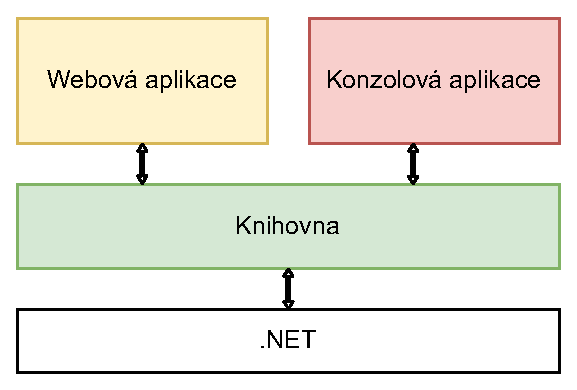
\includegraphics[width=95mm,scale=0.5]{Figures/obrazky/Programlayers.eps}
    \label{fig:appLayers}
\end{figure}

%Knihovna byla logicky rozvržena do několika částí. 

Průběh statické analýzy byl rozdělen do několika dílčích kroků. Jednotlivé kroky pak zabezpečují samotné moduly programu, kterých bylo v této práci vytvořeno celkem sedm.

Každý konkrétní modul provádí samostatný proces a je zcela nezávislý na modulech ostatních. To umožňuje kdykoliv přidat nebo odebrat některý z těchto modulů a případně knihovnu rozšířit o moduly nové.

Všechny vytvořené moduly implementují přetíženou metodu \emph{ToString}, která následně umožňuje snazší práci s výstupem aplikace.

Některé často používané funkcionality pro práci s řetězci a kolekcemi jsou implementovány formou externích rozšíření.

\paragraph*{Moduly}
\label{modules_app}

Implementovány byly následující moduly. Pořadí popisu modulů pak odpovídá jednotlivým krokům statické analýzy.

\subparagraph*{MIME} 

Prvním krokem statické analýzy je detekce typu MIME. Tu zajišťuje knihovna \emph{MIME} viz kapitola \ref{lib_mime}.

Nejprve je vytvořena instance třídy pro zjištění tohoto typu a poté se zavolá potřebná metoda, jež slouží k zjištění typu.
 
\subparagraph*{Hashes}

Tento modul zajišťuje výpočet několika různých hašovacích funkcí, a to konkrétně MD5, SHA-1, SHA-256, SHA-384, SHA-512.
Tyto funkce slouží primárně pro možnost případného vyhledání vzorku v různých databázích malwaru.

Z veřejných databází lze využít například databázi \emph{Malshare.com}, případně již dříve zmíněný VirusTotal.

\subparagraph*{VirusTotal}

Dalším modulem je modul pro aplikaci VirusTotal, předání pak zajišťuje knihovna \emph{VirusTotalNET} (viz kapitola \ref{virustotal_lib}).

Zpracování a odeslání dat službě VirusTotal, je velmi jednoduché a to proto, že většinu funkční části zajišťuje samotná knihovna. 

Nejprve je vytvořena instance třídy \emph{VirusTotal}. Pro komunikaci se službou VirusTotal je zapotřebí mít vytvořený účet v této službě a zaregistrovat si vlastní API klíč (jedná se o klíč pro programovatelné rozhraní služby, jež slouží k autorizaci požadavků). V základním režimu je~možné odeslat k testování 4 požadavky za minutu a 1000 požadavků denně.

Pokud již byla vytvořena instance, může následovat testování daného vzorku. Nejprve je~provedeno vyhledání v databázi již existujících výsledků testů. Pokud vzorek testován dosud nebyl, je odeslán k testu. Dalším omezením může být velikost souboru. Její horní hranice ve~veřejném API je 32 MB.

\subparagraph*{Entropie}

Následuje krok, ve kterém je vypočtena entropie pro zkoumaný soubor. Výsledek pak může naznačovat, zda bylo provedeno šifrování nebo komprese souboru \cite{sikorski2012practical}. 

V daném případě se provede výpočet pomocí následujícího vzorce \ref{vypocetEntropie}, který je aplikován na~načtený soubor v paměti jako pole bytů. 

\begin{equation}
    \label{vypocetEntropie}
    En=-\sum_{n=1}^{\infty} f_n * \frac{\log{f_n}}{\log{2}}
\end{equation}

\begin{equation}
    \label{vypocetEntropie_sub}
    f_n= \frac{p}{c}
\end{equation}

Kde $p =$ počet výskytu stejného bytu a $c =$ celková délka pole bytů.

Čím více se výsledná hodnota entropie ($En$) blíží číslu 8, tím více je pravděpodobné, že~se jedná o šifrovaný nebo komprimovaný soubor \cite{entropy}.

% vypočítám entropií
% což mi říká to a to blablablabla

Ukázku výsledné entropie prezentuje následující tabulka č. \ref{entropy_table}. Pro testování byl zvolen multimediální přehrávač VLC. Nejdříve bylo provedeno packování pomocí známého packeru pro kompresi UPX a komerečního packeru ASPack a následně byla vypočtena entropie jednotlivých souborů.

\begin{table}[H]
    \centering

    \begin{tabular}{|l|l|l|}
        \hline
            & Entropie & Velikost souboru \\ \hline \hline
         bez komprese   &   6.47 & 940 kB \\ \hline
         UPX            &   7.83 & 324 kB \\ \hline
         ASPack         &   7.85 & 316 kB \\ \hline
    \end{tabular}
    
    \caption{Ukázka entropie packerů UPX a ASPack}
    \label{entropy_table}
\end{table}

\subparagraph*{PE}

Modul PE zajišťuje analýzu hlavičky spustitelných souborů PE (viz kapitola č. \ref{pe_format}) a~to~za pomoci knihovny PeNET (viz kapitola \ref{penet_lib}).

Nejprve je generována instance třídy \emph{PeFile} z knihovny PeNET. Ta zajišťuje veškerou práci se strukturou PE souboru, jako jsou zjištění jednotlivých sekcí, importů knihoven, funkcí atd. 

Následně se pro zjednodušení práce s PE strukturou načtou do vlastní třídy modulu \emph{PE} importy, exporty, directories a sekce (viz kapitola \ref{pe_format}).

Modul obsahuje implementaci pro zjištění jak základních parametrů jako je adresa vstupního bodu (angl. entry point) programu, velikost, čas vytvoření, typ a zda se jedná o knihovnu DLL, ovladač nebo EXE soubor. Ale také pokročilejší informace o importovaných a exportovaných funkcích a knihovnách, seznam sekcí a jejich parametrů nebo seznam jednotlivých directories. 

Ukázku výstupu lze vidět na následujícím obrázku \ref{fig:consolePeResult}.

\begin{figure}[H]
    \caption{Ukázka výstupu informací o spustitelném souboru formátu PE}
    \centering
    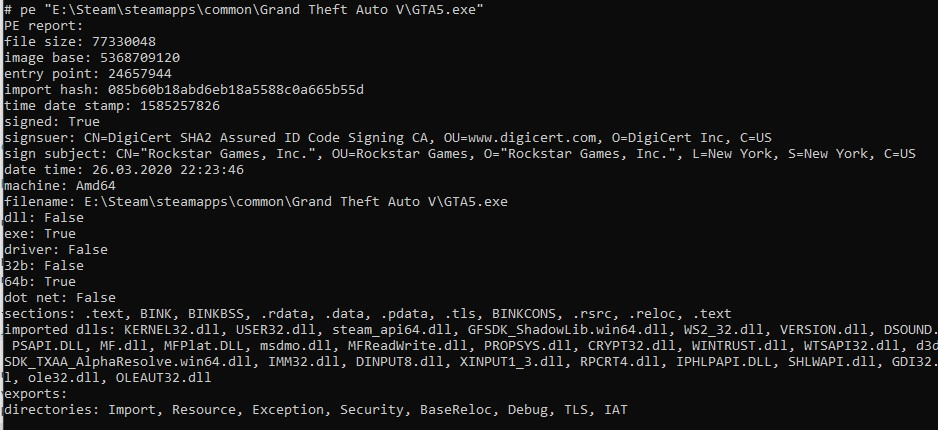
\includegraphics[width=160mm,scale=0.5]{Figures/obrazky/konzole-pe.jpg}
    \label{fig:consolePeResult}
\end{figure}

% co zkoumám
% co k tomu používám
% co si ukládám
% co mě zajimá

\subparagraph*{Strings}

Analýza řetězců probíhá v modulu \emph{Strings}. Průběh analýzy je rozdělen do několika kroků.
Nejprve je načten soubor do paměti a převeden na řetězec.
Poté je provedena filtrace nepožadovaných znaků (netisknutelné znaky, konec řetězce atp.), tyto znaky jsou odstraněny z toho důvodu, aby byla zajištěna lepší čitelnost výstupu při ruční analýze.

Následně je vyhledán název souborů uložených v programu pomocí vygenerovaného regulárního výrazu. Ten je vytvořen na základě získaného seznamu MIME typů (přípon souboru). Tento seznam je nejdříve načten do paměti z JSON souboru. Poté je provedeno vygenerování regulárního výrazu \emph{..(.jpg|.png ... |.exe)..} a vytvořena instance pro vyhledání jednotlivých výskytů v testovaném souboru. Zjištěná data jsou vrácena formou seznamu.

Dále je provedeno vyhledání důležitých informací, které mohou sloužit malwaru jako způsob, jak informovat útočníka o stavu útoku nebo naopak jako zdroj úkolu pro program, například vzdálená aktivace DDoS (Denial of service - útok s cílem zahltit požadovaný cíl) apod. Konkrétně se může jednat o IP adresy, emaily nebo informace ve formátu URL adresy jako \emph{https://}, \emph{smb://} nebo například \emph{ftp://}.

Vyhledání těchto dat se opět provádí pomocí regulárního výrazu, v tomto případě se pak jedná o předem vytvořené a uložené konstanty.

Posledním krokem analýzy je vyhledání známých metod používaných malwarem. Jako je například volání Windows API, Anti-debuggování atd. Seznam těchto metod byl získán z GitHub repositáře \emph{Cisco-Talos/Bass}. Vyhledání těchto metod je prováděno pomocí metody \emph{Contains}. Pokud je požadovaný řetězec obsažen, přidá se do seznamu.

% co zkoumám a jak
% zajimavosti o tom

\subparagraph*{Detect with Yara}

Pro detekci dalších vlastností byl vytvořen modul, který zajišťuje analýzu pokročilejších vlastností jako například kontrolu signatur různých packerů, výskyt různých metod chování na základě obsažené kombinace knihoven nebo detekci obranných mechanismů vůči analýze.

Pro tuto detekci, jsou použity již vytvořená pravidla z veřejného repositáře \emph{Yara-rules/rules} na platformě pro sdílení GIT repositářů Github.

A jsou to konkrétně pravidla pro detekci důležitých vlastností jako například obrana vůči debuggování nebo virtuálnímu prostředí. Dále to pak jsou pravidla pro detekci známých signatur packerů nebo kompilátorů.

%%%%%%%%%%%%%%%%%%%%%%%%%%%%%%%%%%%%%%%%%%%
\subsection{Výstup aplikace}

Pro zajištění výstupu je v knihovně \emph{StaticAnalysisProject.Lib} implementována třída \emph{FileReport}. Třída \emph{FileReport} zajišťuje veškerou inicializaci instancí jednotlivých modulů a zpracování dat z~jednotlivých části statické analýzy testovaného vzorku.

Řešení pak obsahuje implementaci dvou odlišných přístupů pro výstup aplikace. A to jako webová nebo konzolová aplikace. Ty jsou popsány v následujícím textu.

\paragraph*{Konzolová aplikace}

Rozhraní konzolové aplikace je koncipováno jako interaktivní uživatelský příkazový řádek. Po spuštění aplikace je uživatel uveden do prostředí programu, kde pomocí zápisu textových příkazů může tuto aplikaci ovládat.

Příkazy v programu jsou uzpůsobeny tak, že je možné provést buď jednotlivé kroky statické analýzy pomocí modulů této aplikace (viz kapitola \ref{modules_app}), anebo provést kompletní analýzu a získat tak výstup.

Na následujícím obrázku č. \ref{fig:consoleAppResult} lze vidět výstup interaktivního prostředí konzolové aplikace.

\begin{figure}[H]
    \caption{Ukázka výstupu konzolové aplikace}
    \centering
    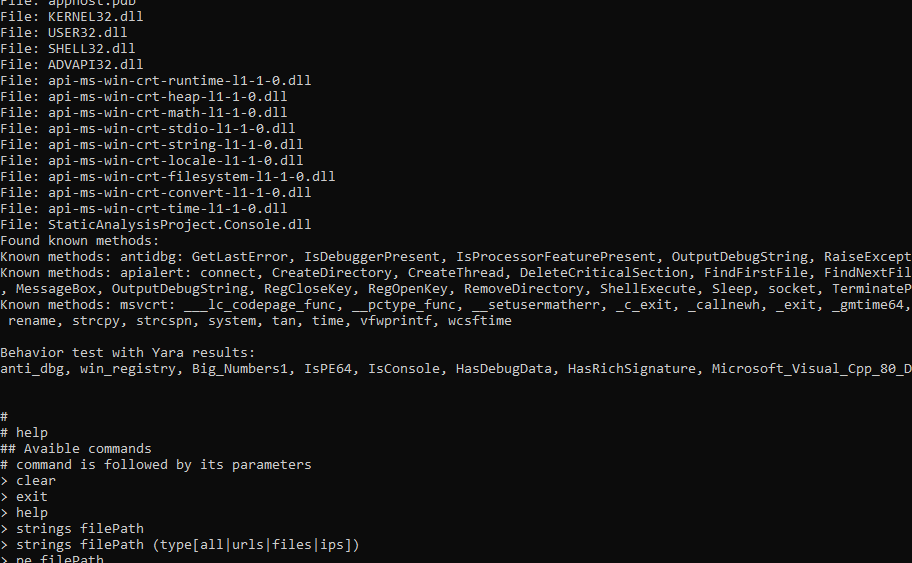
\includegraphics[width=160mm,scale=0.5]{Figures/obrazky/konzole.png}
    \label{fig:consoleAppResult}
\end{figure}

Další možností je pak spuštění aplikace s parametry, kdy lze získat přímý výstup bez nutnosti vstupovat do interaktivního prostředí programu.

\subparagraph*{Práce s aplikací}

Po spuštění se uživatel ocitne v interaktivním prostředí konzolové aplikace, kde může začít zadávat příkazy viz obrázek č. \ref{fig:consoleWork1}.

\begin{figure}[H]
    \caption{Práce s konzolovou aplikací - spuštění}
    \centering
    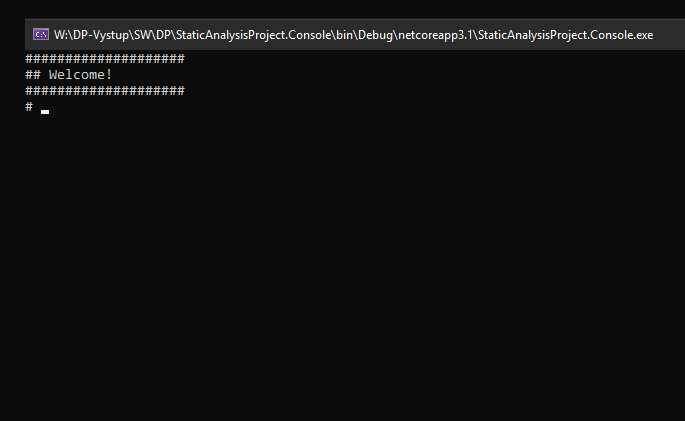
\includegraphics[width=135mm,scale=0.5]{Figures/obrazky/konzole-krok1.png}
    \label{fig:consoleWork1}
\end{figure}

Prvním příkazem, který může uživatel využít je příkaz \emph{help}, který zobrazí nápovědu (seznam použitelných příkazů) (viz obrázek č. \ref{fig:consoleWork2}).

\begin{figure}[H]
    \caption{Práce s konzolovou aplikací - příkaz help}
    \centering
    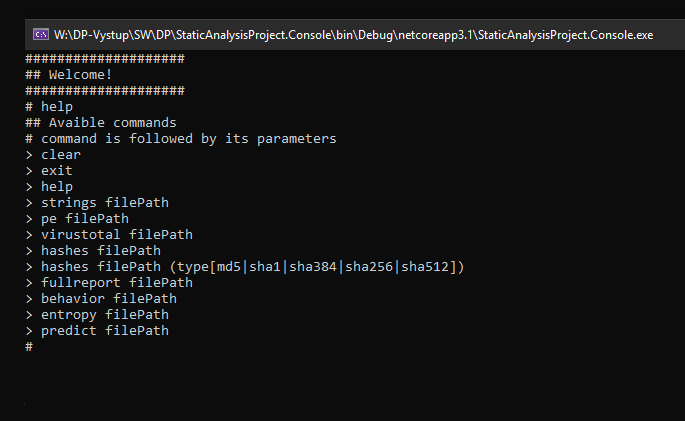
\includegraphics[width=135mm,scale=0.5]{Figures/obrazky/konzole-krok2.png}
    \label{fig:consoleWork2}
\end{figure}

Pokud je potřeba provést analýzu pomocí nástroje \emph{Yara}, použijeme příkaz \emph{behavior} viz obrázek č.~\ref{fig:consoleWork3}. Výstupem pak je seznam pozitivních pravidel, které mohou naznačovat chování aplikace. 

\begin{figure}[H]
    \caption{Práce s konzolovou aplikací - test pomocí Yara}
    \centering
    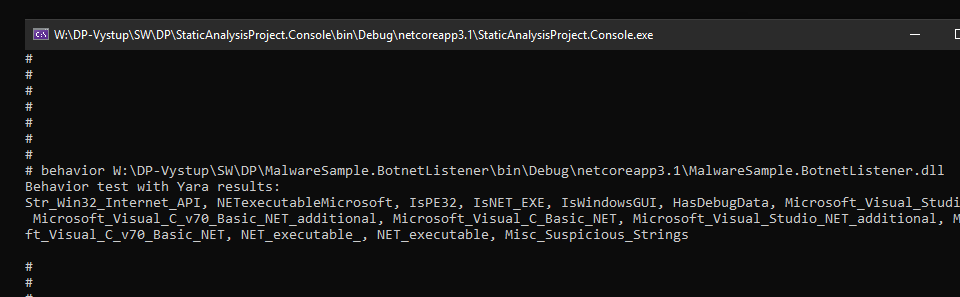
\includegraphics[width=135mm,scale=0.5]{Figures/obrazky/konzole-krok3.png}
    \label{fig:consoleWork3}
\end{figure}

Dalším příkazem pak může být testování službou \emph{VirusTotal}, která provede skenování různými antivirovými programy. Výstup lze vidět na obrázku č. \ref{fig:consoleWork4}

\begin{figure}[H]
    \caption{Práce s konzolovou aplikací - odeslání na VirusTotal}
    \centering
    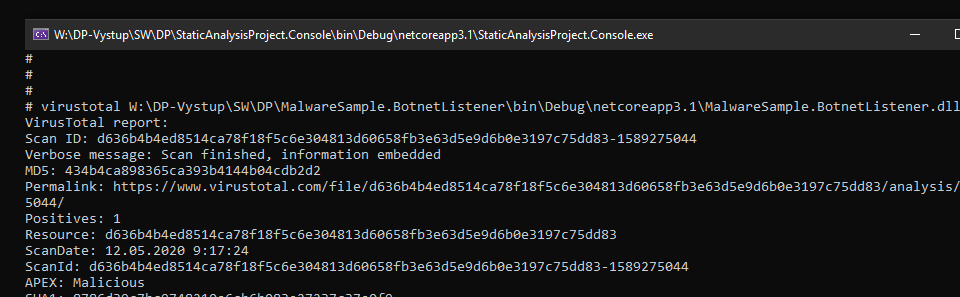
\includegraphics[width=135mm,scale=0.5]{Figures/obrazky/konzole-krok4.png}
    \label{fig:consoleWork4}
\end{figure}

\paragraph*{Webová aplikace}

Hlavním cílem vývoje webové aplikace, je možnost jednoduše bez nutnosti instalace dalšího softwaru provést statickou analýzu. 

Uživatelské rozhraní je velmi jednoduché, po otevření webové stránky v prohlížeči stačí zvolit požadovaný soubor. Následně je provedeno odeslání na webový server, kde je provedena statická analýza obdobně jako u konzolové aplikace s plným výstupem.

Uživatel tak může vidět kompletní výstup statické analýzy. Součástí výstupu je také výsledek binární klasifikace provedené pomocí knihovny ML.NET (viz kapitola \ref{ml_net}). Průběh klasifikace je popsán dále v kapitole \ref{app_testing}.

Při vývoji webové aplikace byly použity moderní technologie jako je framework jQuery, který umožňuje snazší vývoj interaktivních webových aplikací. Dále pak rozšíření standardních kaskádových stylů o dynamické funkce LESS a CSS framework Bootstrap ve verzi 4.

Na následujícím obrázku č. \ref{fig:webAppResult} je možné vidět ukázku výstupu webové aplikace. V první části je zvýrazněn výstup klasifikace, který byl dle predikované pravděpodobnosti barevně rozlišen (červená pokud je detekován malware; jestliže malware detekován nebyl a zároveň je pravděpodobnost vyšší než 80 \% je výsledek zobrazen zeleně; v případě, že je pravděpodobnost nižší než 80 \% je zvýrazněn žlutě; pokud má výsledek nižší pravděpodobnost než 20 \% je výsledek šedý).

\begin{figure}[H]
    \caption{Ukázka výstupu webové aplikace}
    \centering
    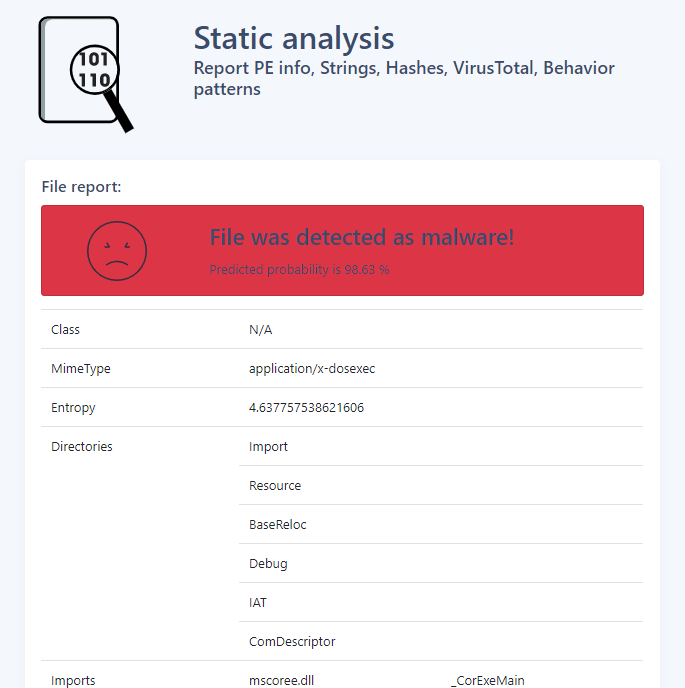
\includegraphics[width=135mm,scale=0.5]{Figures/obrazky/web.png}
    \label{fig:webAppResult}
\end{figure}

\subparagraph*{Práce s aplikací}

Po vstupu na webovou stránku je uživateli zobrazen webový formulář, kde je vyzván k výběru požadovaného souboru viz \ref{fig:workWithWebApp1}.

\begin{figure}[H]
    \caption{Práce s webovou aplikací krok 1.}
    \centering
    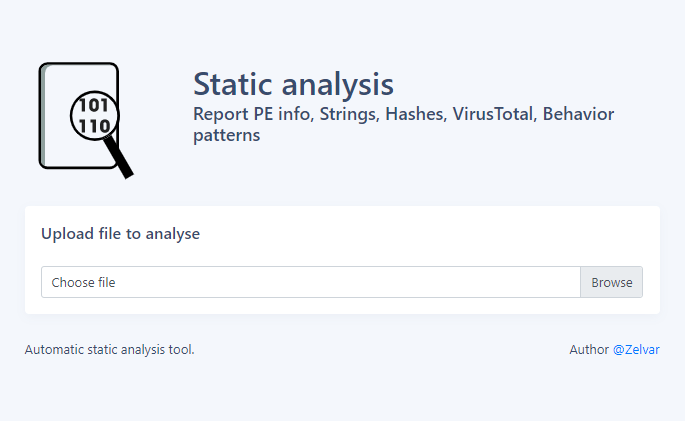
\includegraphics[width=135mm,scale=0.5]{Figures/obrazky/web-krok1.png}
    \label{fig:workWithWebApp1}
\end{figure}

Následně je vybrán požadovaný soubor pro testování viz obrázek č. \ref{fig:workWithWebApp2} a poté potvrzen výběr souboru.

\begin{figure}[H]
    \caption{Práce s webovou aplikací krok 2.}
    \centering
    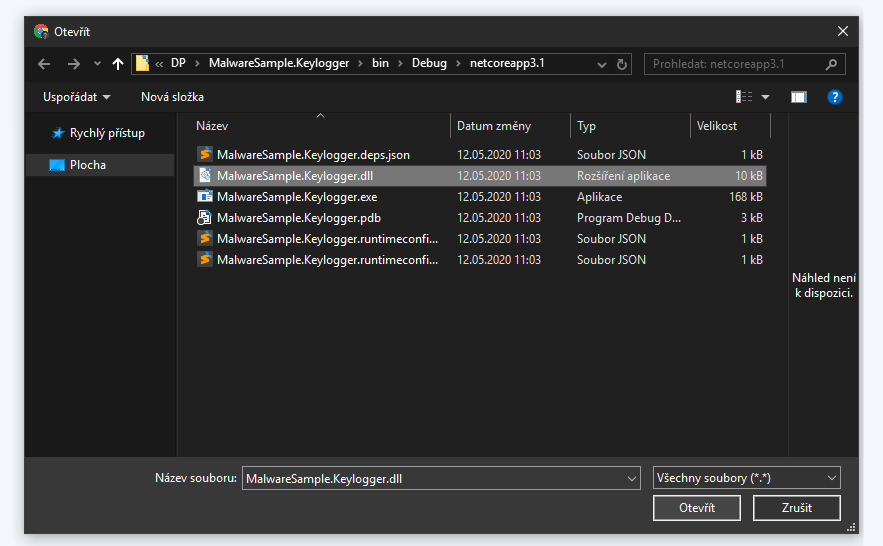
\includegraphics[width=135mm,scale=0.5]{Figures/obrazky/web-krok2.png}
    \label{fig:workWithWebApp2}
\end{figure}

Aplikace poté zpracuje analýzu požadovaného souboru a zobrazí ji uživateli, což je vidět na obrázku č. \ref{fig:workWithWebApp3}.

\begin{figure}[H]
    \caption{Práce s webovou aplikací krok 3.}
    \centering
    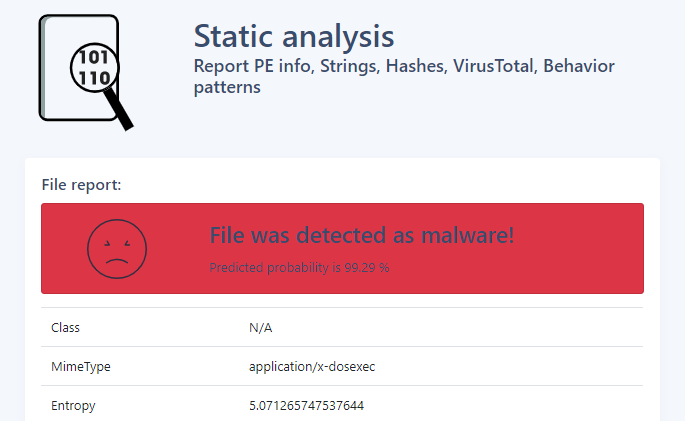
\includegraphics[width=135mm,scale=0.5]{Figures/obrazky/web-krok3.png}
    \label{fig:workWithWebApp3}
\end{figure}

%%%%%%%%%%%%%%%% SUBKAPITOLA Testování
\subsection{Testování aplikace}
\label{app_testing}

V průběhu vývoje programu byla aplikace testovaná na různých kategorií souborů. Především bylo testování zaměřeno na malware. Testování je pak konkrétněji popsáno dále v této kapitole.

%% TODO??
%\paragraph*{Porovnání s aplikacemi pro statickou analýzu}
%PeStudio atd?

\paragraph*{Testování malwaru}

%Za tímto účelem bylo z veřejně dostupných databází získán malware. Tento malware dále posloužil také jako vhodný zdroj informací pro vytvoření kolekce dat (angl dataset), jež měl sloužit jako zdroj informací pro strojové učení. 

Testování malwaru bylo prováděno formou analýzy zvolených souborů. Průběh této analýzy je zmíněn již v kapitole \ref{process_analysis}. Tato kapitola se dále zaměří pouze na testování malwaru určeného pro operační systém Windows ve formátu PE (viz kapitola \ref{pe_format}).

Aby analýza malwaru mohla být vůbec provedena, je nejprve zapotřebí vytvořit nebo získat vzorky malwaru. 

Za tímto účelem je z veřejně dostupných databází malwaru získáno 1952 vzorků, které jsou následně automaticky analyzovány pomocí vytvořeného programu. Tento malware také dále slouží jako vhodný zdroj informací pro vytvoření kolekce dat (angl. dataset), který má i funkci vstupního zdroje informací pro strojové učení. 

Již zmíněné databáze malwaru lze nalézt na webové adrese \url{https://dasmalwerk.eu} a~dále pak na GitHubu, konkrétně v repositáři \emph{ytisf/theZoo}.

Tak, aby bylo možné maximálně automatizovat skenování velkého množství dat, je vytvořen jednoduchý program. Tento program zajišťuje vyhledání souborů v požadované cestě určené při spuštění programu.

Program zároveň zajišťuje aby nedošlo k překročení omezení API služby \emph{VirusTotal}, která v základním tarifu nedovoluje více než 4 požadavky za minutu a 1000 požadavků za jeden den. V základním režimu je také omezena velikost souboru na 32 MB \cite{virustotal_limit}.

Nakonec se výsledky analýzy zaznamenávají do jednoho souboru ve formátu \emph{JSON}, který je~následně použit jako zdroj informací.

Pro porovnání bylo do datasetu také vloženo 108 výstupu legitimních aplikací (dále nazývané jako software). Při výběru je brán zřetel na nutnost různorodosti jednotlivých vlastností. Proto je vybráno několik podskupin jako například hry, správce souborů, kancelářské programy ale~také peněženky pro virtuální měny atd. Tato část kolekce je dále nazývána jako software.

%   U těchto vzorků bylo zjištěno ... STATISTIKA YARA + knihovny / fukce atd.
% https://docs.google.com/spreadsheets/d/1OwhYbQDeQnYJ14F48OLJ-BSLlGOWhqZMJ55G7Bl7-C8/edit#gid=0

%%%%%%%%%%%%%%%%%% STATS!!!!!!! TODO

Následující tabulka č. \ref{table:mimetypes_table} prezentuje podíl spustitelných souborů pro OS Windows, detekovaný pomocí modulu \emph{MIME} (viz kapitola \ref{modules_app}) obsažený v datové kolekci.

%application/x-dosexec
\begin{table}[H]
    \caption{Podíl spustitelných souborů v datasetu}
    \label{table:mimetypes_table}
    
    \centering
    \begin{tabular}{|l|l|l|}
        \hline
                            & Software & Malware       \\
        \hline
    	\hline
        PE (.exe, .dll)      & 108     & 769   \\ \hline
        jiný                 & 0       & 1183  \\ \hline
        celkem               & 108     & 1952  \\ \hline
    \end{tabular}
\end{table}

Vzhledem k tomu, že se práce zabývá primárně malwarem určeným pro operační systém Windows, jsou dále zohledňována a uváděna data pouze pro malware útočící právě na tento OS.

%%%%%%%%%% VLASTNOSTI PE
Tabulka č. \ref{table:pefile_table} demonstruje podíl jednotlivých parametrů spustitelných PE souborů v datové kolekci. Parametry \emph{16b}, \emph{32b} a \emph{64b} určují pro jakou architekturu procesoru je program určen, zda se jedná o 32 nebo 64 bitový systém. Vzhledem k tomu, že 64 bitový systém podporuje také spouštění 32 bitových aplikací. Útočnici mohou stále vytvářet škodlivý kód pro zajištění kompatibility s 32 bitovou verzí systému. Zároveň lze však dle statistik \emph{PassMark Software} očekávat sestupný podíl malwaru pro 32 bitovou platformu. A to převážně z důvodu klesajícího počtu instalací 32 bitových Windows \cite{passmark_32_stats}. 

Podíl podepsaného (Signed) škodlivého kódu nebo malwaru skrytého jako ovladače není často velký. Část nativního kódu převažuje nad kódem interpretovaným alespoň v případě platformy .NET.

\begin{table}[H]
    \caption{Parametry spustitelných souborů v kolekci dat}
    \label{table:pefile_table}
    
    \centering
    \begin{tabular}{|l|l|l|}
        \hline
               & Software & Malware \\ 
        \hline
        \hline
        16b    & 0.00 \%   & 1.56 \%  \\ \hline
        32b    & 50.00 \%  & 96.10 \% \\ \hline
        64b    & 50.00 \%  & 2.34 \%  \\ \hline
        DLL    & 21.30 \%  & 5.85 \%  \\ \hline
        EXE    & 78.70 \%  & 91.81 \% \\ \hline
        .NET   & 4.63 \%   & 15.08 \% \\ \hline
        Driver & 0.00 \%   & 0.13 \%  \\ \hline
        Signed & 33.33 \%  & 11.44 \% \\ \hline
    \end{tabular}
\end{table}

%%%%%%%%%%% SEKCE PE
Další tabulka č. \ref{table:sections_table} pak prezentuje střední hodnoty počtů sekcí spustitelných PE souborů v~jednotlivých skupinách. Na základě těchto dat lze usuzovat, že malware disponuje průměrně menším počtem sekcí než běžný software. 

\begin{table}[H]
    \caption{Počty sekcí v jednotlivých skupinách}
    \label{table:sections_table}
	
	\centering
	\begin{tabular}{|l|l|l|}
		\hline
		       & Software & Malware \\ 
		\hline
		\hline
		Průměr & 7.34     & 4.81    \\ \hline
		Medián & 7.00        & 4.00       \\ \hline
		S.D.   & 3.03     & 1.9    	\\ \hline
	\end{tabular}
\end{table}

%%%%%%%%%%%% Entropie graf + tabulka

\begin{table}[H]
    \caption{Entropie jednotlivých skupin}
    \label{table:entropie_table}
    
    \centering
	\begin{tabular}{|l|l|l|}
		\hline
		                    & Software & Malware \\
		\hline
		\hline
		Průměr              & 6.38     & 6.97                  \\ \hline
		Medián              & 6.41     & 7.08                  \\ \hline
		Směrodatná odchylka & 0.94     & 1.00                  \\ \hline
	\end{tabular}
\end{table}

Následující graf na obrázku č. \ref{fig:entropie} obsahuje četnosti hodnot entropie pro software a malware. Pro~lepší orientaci byla entropie zaokrouhlena v kroku 0.5. Hodnoty entropie softwaru vykazují na hladině spolehlivosti 98 \% normální rozložení naopak u hodnot entropie pro malware lze pozorovat extrém entropie v hodnotě 6.0 a druhý v hodnotně 8.0. Zároveň je z tabulky 9 patrné, že průměrné hodnoty entropie a také jejího mediánu jsou pro malware vyšší než pro software. To,~že~se~hodnoty statisticky významně liší, bylo prokázáno i za použití Mann-Whitneyova U-testu. 

\begin{figure}[H]
    \noindent
    \centering
    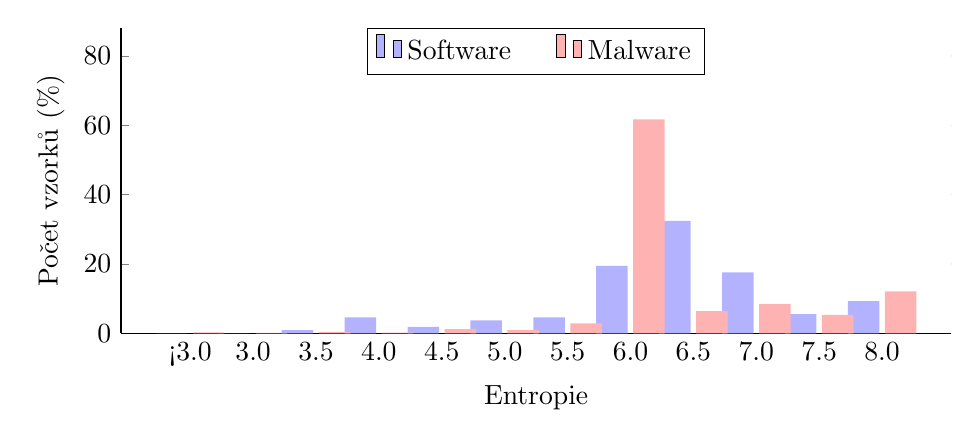
\begin{tikzpicture}
    \centering
    \begin{axis}[
                ybar,
                bar width=0.4cm, 
                width=\textwidth,
                height=.45\textwidth,
                ymajorgrids, tick align=inside,
                major grid style={draw=white},
                enlarge y limits={value=.1,upper},
                ymin=0, ymax=80,
                axis x line*=bottom,
                axis y line*=left,
                yminorgrids = true,
                y axis line style={opacity=100},
                tickwidth=0pt,
                enlarge x limits=true,
                legend style={
                    at={(0.5,1)},
                    anchor=north,
                    legend columns=-1,
                    /tikz/every even column/.append style={column sep=0.5cm}
                },
                minor ytick={0,20,...,100},
                grid=both,
                ylabel={Počet vzorků (\%)},
                xlabel={Entropie},
                symbolic x coords={<3.0,3.0,3.5,4.0,4.5,5.0,5.5,6.0,6.5,7.0,7.5,8.0},
               xtick=data,
               nodes near coords={
                %\pgfmathprintnumber[precision=0]{\pgfplotspointmeta}
               }
            ]
        \addplot [draw=none, fill=blue!30] coordinates {(<3.0, 0.00)(3.0, 0.00)(3.5, 0.93)(4.0, 4.63)(4.5, 1.85)(5.0, 3.70)(5.5, 4.63)(6.0, 19.44)(6.5, 32.41)(7.0, 17.59)(7.5, 5.56)(8.0, 9.26)};
        \addplot [draw=none, fill=red!30] coordinates {(<3.0, 0.26)(3.0, 0.15 )(3.5, 0.41 )(4.0, 0.20 )(4.5, 1.18 )(5.0, 0.92 )(5.5, 2.87 )(6.0, 61.73)(6.5, 6.40 )(7.0, 8.45)(7.5, 5.33)(8.0, 12.09)};
        \legend{Software, Malware}
    \end{axis}
    \end{tikzpicture}
    
    \caption{Entropie vzorků}
    \label{fig:entropie}
\end{figure}

%%%%%%%%%%% ŘETĚZCE

Dalším zjišťovaným parametrem (viz tabulka č. \ref{table:strings_table}) byla informace, jež určovala zda testovaný vzorek obsahuje konkrétní typ řetězce. V tomto případě se jednalo o \emph{email}, \emph{ip adresu} (jak IPv4 tak IPv6) a \emph{url adresu}. Zajímavým zjištěním je, že v případě malwaru je výskyt \emph{emailové} a~\emph{url} adresy nižší. V případě malwaru mohou tyto informace, které slouží často ke komunikaci s~útočníkem skryté pomocí různých obfuskačních metod viz kapitola \ref{obfuskacni_metody}. 

\begin{table}[H]
	\caption{Výskyt konkrétního typu řetězce}
	\label{table:strings_table}

    \centering
	\begin{tabular}{|l|l|l|}
	 	\hline
		     & Software & Malware \\
		\hline
		\hline
		Mail & 53.70 \%   & 26.80 \%  \\	 \hline
		IP   & 94.40 \%   & 87.30 \%  \\	 \hline
		URL  & 85.20 \%   & 34.30 \%  \\	 \hline
	\end{tabular}
\end{table}

%%%%%%%%%%% DLL
Následující data v tabulce č. \ref{table:libs_table} prezentují patnáct nejpoužívanějších knihoven v kolekci dat, používané jak softwarem tak malwarem. Na datech můžeme jasně vidět, že se použité knihovny se~velmi podobají a rozlišit malware od legitimních aplikací (software) pouze pomocí této informace není možné. Proto se tato informace kombinuje se seznamem použitých metod, které jsou volány z těchto knihoven. 

\begin{table}[H]
    \caption{Porovnání výskytu použitých knihoven}
    \label{table:libs_table}

    \centering
    \begin{tabular}{|l|l|l|l|}
        \hline
        \multicolumn{2}{|l|}{Software}                & \multicolumn{2}{|l|}{Malware} \\ \hline
        Knihovna                          & Výskyt  & Knihovna        & Výskyt    \\ 
        \hline
    	\hline
        kernel32.dll                      & 92.59 \% & kernel32.dll    & 76.98 \%   \\ \hline
        user32.dll                        & 75.00 \% & user32.dll      & 60.99 \%   \\ \hline
        advapi32.dll                      & 73.15 \% & advapi32.dll    & 59.82 \%   \\ \hline
        shell32.dll                       & 68.52 \% & gdi32.dll       & 38.75 \%   \\ \hline
        gdi32.dll                         & 57.41 \% & shell32.dll     & 36.80 \%   \\ \hline
        ole32.dll                         & 56.48 \% & ole32.dll       & 35.37 \%   \\ \hline
        oleaut32.dll                      & 44.44 \% & comctl32.dll    & 33.29 \%   \\ \hline
        comctl32.dll                      & 38.89 \% & oleaut32.dll    & 23.41 \%   \\ \hline
        version.dll                       & 37.96 \% & version.dll     & 21.07 \%   \\ \hline
        shlwapi.dll                       & 32.41 \% & ws2\_32.dll     & 19.25 \%   \\ \hline
        winmm.dll                         & 24.07 \% & mscoree.dll     & 14.95 \%   \\ \hline
        ws2\_32.dll                       & 22.22 \% & msvcrt.dll      & 14.95 \%   \\ \hline
        comdlg32.dll                      & 21.30 \% & shlwapi.dll     & 13.26 \%   \\ \hline
        vcruntime140.dll                  & 18.52 \% & wininet.dll     & 13.26 \%   \\ \hline
        api-ms-win-crt-runtime-l1-1-0.dll & 18.52 \% & comdlg32.dll    & 9.36 \%    \\ \hline
    \end{tabular}
\end{table}

%%%%%%%%% FUNKCE
Seznam patnácti nejpoužívanějších metod je pak možné vidět v následující tabulce č. \ref{table:methods_table}, kde je opět vidět jistou podobnost mezi softwarem a malwarem. Rozdíl ve volaných funkcích je však větší. Prvním příkladem může být metoda \emph{GetModuleHandleA}, kterou malware využívá k nalezení vhodného místa pro injekci vlastního kódu \cite{method_getmodulehandle}. Příkladem může být například injekce vlastního kódu do kernelu (\emph{GetModuleHandleA(kernel32.dll)}). Dalším metodou častěji používanou malwarem je \emph{LoadLibraryA}. Tato metoda slouží k dynamickému načtení modulu do~adresního prostoru aplikace. Často je také spolu s funkcí \emph{CreateRemoteThread} využívána při technice zvané \emph{DLL Injection} \cite{method_dllinjection}. Tato technika spočívá ve vložení (tzv. injekci) vlastního kódu do běžícího procesu. Tímto postupem může útočník injektovat malware například do procesů operačního systému. 

\begin{table}[H]    
    \caption{Porovnání výskytu použitých metod pro malware a software}
    \label{table:methods_table}
    
    \centering
    \begin{tabular}{|l|l|l|l|}
        \hline
        \multicolumn{2}{|l|}{Software}   & \multicolumn{2}{|l|}{Malware}   \\  \hline
        Funkce               & Výskyt  & Funkce              & Výskyt  \\
        \hline
    	\hline
        GetProcAddress       & 96.30 \% & GetProcAddress      & 81.79 \% \\ \hline
        CloseHandle          & 91.67 \% & WriteFile           & 67.75 \% \\ \hline
        GetCurrentThreadId   & 91.67 \% & GetModuleHandleA    & 65.54 \% \\ \hline
        GetLastError         & 91.67 \% & Sleep               & 64.63 \% \\ \hline
        Sleep                & 90.74 \% & CloseHandle         & 64.50 \% \\ \hline
        GetModuleHandleW     & 90.74 \% & GetLastError        & 63.20 \% \\ \hline
        QueryPerformanc..    & 89.81 \% & ExitProcess         & 62.03 \% \\ \hline
        GetCurrentProcess    & 89.81 \% & LoadLibraryA        & 59.17 \% \\ \hline
        WriteFile            & 87.96 \% & MultiByteToWideChar & 56.31 \% \\ \hline
        WideCharToMultiByte  & 87.04 \% & GetModuleFileNameA  & 52.15 \% \\ \hline
        MultiByteToWideChar  & 87.04 \% & GetTickCount        & 52.15 \% \\ \hline
        FreeLibrary          & 87.04 \% & WideCharToMultiByte & 49.80 \% \\ \hline
        UnhandledExcept..    & 83.33 \% & FreeLibrary         & 49.02 \% \\ \hline
        GetCurrentProcessId  & 81.48 \% & GetCurrentProcess   & 47.20 \% \\ \hline
        GetModuleFileNameW   & 80.56 \% & RegCloseKey         & 46.68 \% \\ \hline
        RegCloseKey          & 78.70 \% & VirtualAlloc        & 46.03 \% \\ \hline
        TerminateProcess     & 77.78 \% & WaitForSingleObject & 43.17 \% \\ \hline
        EnterCriticalSection & 77.78 \% & GetStdHandle        & 43.04 \% \\ \hline
        LeaveCriticalSection & 77.78 \% & ReadFile            & 42.91 \% \\ \hline
        GetSystemTimeAs..    & 76.85 \% & SetFilePointer      & 42.00 \% \\ \hline
    \end{tabular}
\end{table}


%%%%%%%%%%% YARA
Výskyt detekovaných pravidel prezentuje tabulka č. \ref{table:yara_table}. Na výsledných datech lze vidět procentuální výskyt patnácti nejčastějších pravidel, které byly detekovány v obou skupinách. V~případě malwaru můžeme jasně vidět, že bylo nejčastěji detekováno pravidlo (\emph{IsPE32}), které~detekuje 32 bitový spustitelný soubor ve formátu PE. Následují pravidla pro detekci výskytu grafického rozhraní pro Windows \emph{IsWindowsGUI} a pravidlo pro detekci manipulace s práce se soubory pomocí Windows API (\emph{win\_files\_operation}). Oproti běžnému softwaru, bylo u malwaru častěji detekováno pravidlo \emph{IsPacked}, které naznačuje, že u malwaru bylo detekován zabalení packerem (viz kapitola \ref{packers}). Dále pak bylo detekováno pravidlo \emph{SEH\_Init} a \emph{SEH\_Save}, které značí, že zdrojový kód aplikace obsahuje inicializaci pro strukturovanou obsluhu výjimek. V~tomto případě se může jednat o jeden ze způsobu ochrany proti ladění (anti-debug viz kapitola \ref{anti_debug}). Dalším důležitým pravidlem, které bylo detekováno je \emph{escalate\_priv}. Toto pravidlo detekuje způsoby jakým se útočník snaží získat vyšší oprávnění a to tak, aby bylo možné vykonat jinak nerealizovatelný útok \cite{privilage_escl}.

\begin{table}[H]
    \caption{Porovnání detekovaných YARA pravidel}
    \label{table:yara_table}
    
    \centering
    \begin{tabular}{|l|l|l|l|}
        \hline
        \multicolumn{2}{|l|}{Software}          & \multicolumn{2}{|l|}{Malware}                     \\ \hline
        Pravidlo              & Výskyt & Pravidlo                            & Výskyt \\ 
        \hline
        \hline
        IsWindowsGUI          & 75.00 \%       & IsPE32                              & 95.97 \%       \\ \hline
        win\_files\_operation & 64.81 \%       & IsWindowsGUI                        & 93.37 \%       \\ \hline
        HasOverlay            & 60.19 \%       & win\_files\_operation               & 58.00 \%       \\ \hline
        win\_registry         & 59.26 \%       & HasRichSignature                    & 56.18 \%       \\ \hline
        anti\_dbg             & 57.41 \%       & IsPacked                            & 52.93 \%       \\ \hline
        HasRichSignature      & 50.00 \%       & win\_registry                       & 44.21 \%       \\ \hline
        HasDebugData          & 50.00 \%       & SEH\_Init                           & 43.82 \%       \\ \hline
        IsPE32                & 45.37 \%       & HasOverlay                          & 36.02 \%       \\ \hline
        screenshot            & 42.59 \%       & screenshot                          & 33.29 \%       \\ \hline
        CRC32\_poly\_Constant & 42.59 \%       & CRC32\_poly\_Constant               & 30.43 \%       \\ \hline
        IsPE64                & 39.81 \%       & SEH\_Save                           & 29.78 \%       \\ \hline
        win\_token            & 37.04 \%       & MS\_VS\_Cpp\_v50..                  & 28.09 \%       \\ \hline
        win\_mutex            & 37.04 \%       & Str\_Win32\_Wins..                  & 27.05 \%       \\ \hline
        HasDigitalSignature   & 34.26 \%       & win\_token                          & 26.14 \%       \\ \hline
        keylogger             & 31.48 \%       & escalate\_priv                      & 22.11 \%       \\ \hline
    \end{tabular}
\end{table}

\paragraph*{Vlastní malware}
\label{own_malware_dp}

Pro účely testování jsou jako součást práce vytvořeny dva jednoduché druhy malwaru se zcela rozdílným vektorem útoku. Jednotlivé vlastnosti těchto škodlivých programů jsou popsány níže. Tyto vzorky byly primárně použity pro testování klasifikace. Výsledky těchto testů budou popsány dále.

Oba tyto testovací vzorky jsou implementovány v technologií .NET Core jako aplikace s~grafickým rozhraním (zkr. GUI) a to i přes to, že se při spuštění škodlivého programu žádné GUI nevytváří.

\subparagraph*{Botnet}

První ze dvou vzorků funguje na principu velmi jednoduchého klienta sítě, který je vzdáleně ovládán pomocí \emph{CnC} serveru. Klient může vykonávat pouze jednoduchý druh vyřadit službu z provozu (tzv. Denial of service), a to pomocí zasílání pingu z příkazového řádku. V~případě vytvoření větší sítě klientů by se pak mohlo jednat o distribuovaný druh útoku. Princip byl velmi zjednodušen s cílem vytvořit funkční imitaci malwaru. 

Celá síť se ovládá pomocí \emph{Command-and-Control} serveru, jež  byl implementován jako \emph{XML} (angl. Extensible Markup Language) dokument umístěný na webovém serveru. Tento dokument obsahuje cíl útoku (IP adresu) a informaci o aktivaci (zapnuto nebo vypnuto).

\subparagraph*{Keylogger}

Druhým škodlivým programem je pak aplikace pro skryté zaznamenávání stisku klávesnice a odesílání na webový server. Aplikace se po spuštění zavěsí na potřebné \emph{Windows API}, které slouží k získávání informací o stisku kláves a následně je vyvolávána při stisku volitelné klávesy událost, jež má za úkol zaznamenat stisknutý znak do proměnné. 

Pokud již bylo zaznamenáno 100 znaků, informace (zaznamenané stisky kláves) se odešlou na webový server, kde jej jednoduchý \emph{PHP} skript zaznamená do textového souboru.

V případě, že uživatel například použije platební kartu na internetu a útočník zaznamená jeho stisky kláves, mohou být jím zadané údaje následně zneužity.

%%%%%%%%%%%%%

\paragraph*{Klasifikace výstupu analýzy}

Klasifikace výstupu probíhala pomocí výše zmíněné technologie \emph{ML.NET} (viz kapitola \ref{ml_net}), která umožňuje snadné nasazení strojového učení na téměř jakoukoliv aplikaci.

Pro nasazení strojového učení stačí přidat do modelu, který obsahuje data, k jednotlivým proměnným parametr \emph{[LoadColumn(x)]} (kde \emph{x} je pořadí sloupce). Tím zajistíme možnost využít data pro strojové učení. Protože však technologie podporuje pouze některé datové typy (řetězce, boolean, float, vektorové data atd.) bylo potřeba data předzpracovat do požadovaného formátu. Proto byl model značně zjednodušen a obsahuje pouze některé parametry z výstupu statické analýzy.

Těmito parametry jsou základní vlastnosti PE hlavičky jako typ (Ovladač, \emph{DLL}, \emph{EXE}, platforma), zda je aplikace podepsaná digitálním certifikátem, třída (malware nebo software), entropie, detekované řetězce (\emph{email}, \emph{IP} a \emph{URL}), počet pozitivních testů \emph{VirusTotal}, seznam používaných metod a knihoven a zjištěné pozitivní výsledky pravidel \emph{Yara}.

Následně je provedeno automatické trénování (učení s učitelem) klasifikačního modelu pomocí vytvořené kolekce dat. Pro trénování je použito 80 \% dat datové kolekce, zbylých 30~\% je~použito pro křížovou validaci s deseti opakováními. Křížová validace má za úkol zjistit (vyhodnotit) jak moc jsou ovlivňovány nezávislé vzorky dat \cite{crossvalidation}.

Pro trénování byl použit algoritmus \emph{SdcaLogisticRegression}, který má zajistit dobré výsledky bez nutnosti jej dále ladit \cite{ms_mlnettraining}. Aby bylo možné tento algoritmus použít, je potřeba data nejdříve normalizovat. Pro tuto transformaci se využívá metoda \emph{NormalizeBinning}.

Součástí vypracovaní této diplomové práce je již vygenerovaný model na základě datové kolekce, která je také součástí. V případě však, že dojde ke změně dat je nutné tento model odstranit a nechat jej program vygenerovat znovu.

Následně se tento vytrénovaný model použije pro predikci třídy (software nebo malware), testovaného vzorku na základě výstupu statické analýzy.

\subparagraph*{Testování}
\label{my_malware_tests}

Pro testování byly použity výše zmíněné vzorky malwaru, které byly vytvořeny jako součást této práce (viz kapitola \ref{own_malware_dp}). A dvacet legitimních aplikací a dvacet dalších vzorků malwaru z databáze \emph{VirusShare.com}. Tyto vzorky nebyly použity při vytváření datové kolekce.

Následující tabulka č. \ref{table:my_malware} prezentuje výsledky testování vlastního malwaru. Jak lze vidět, malware byl detekován s přesností přes 90 \%. A oba vzorky byly pozitivně testovány. Úspěšnost je tedy 100 \%.

\begin{table}[H]
    \centering
    \begin{tabular}{|l|l|l|}
        \hline
        Soubor & Detekováno & Pravděpodobnost\\ \hline
        \hline
        KeyLogger.dll	&	Ano	&	91.34 \% \\ \hline
        BotnetListener.dll	&	Ano	&	93.71 \% \\ \hline
    \end{tabular}
    \caption{Detekce vytvořeného malwaru}
    \label{table:my_malware}
\end{table}

Další testování je provedeno na malwaru z databáze \emph{VirusShare.com}. Z této databáze je staženo 20 vzorků, které jsou podrobeny testům. Tabulka č. \ref{table:virusharae_malware} obsahuje část kontrolního součtu vytvořeného pomocí \emph{SHA-256} (kompletní kontrolní součty jsou pak součástí přílohy), název pod kterým byl detekován antivirem \emph{Avast}, zda byl detekován a s jakou pravděpodobnosti. V tomto případě je úspěšnost testování 100 \%.

\begin{table}[H]
    \centering
	\begin{tabular}{|l|l|l|l|}
		\hline
		SHA256    & Avast              			   & Detekováno & Pravděpodobnost \\ \hline
		\hline
		cbfc9d3.. & Undetected                     & Ano  & 99.99 \% \\ \hline
		8757088.. & Undetected                     & Ano  & 99.99 \% \\ \hline
		000ad60.. & Win32:PUP-gen {[}PUP{]}        & Ano  & 99.99 \% \\ \hline
		037bfec.. & Win32:AdwareSig {[}Adw{]}      & Ano  & 100 \% \\ \hline
		0872a6c.. & Win32:VBCrypt-AKV {[}PUP{]}    & Ano  & 99.99 \% \\ \hline
		190ea43.. & Win32:Downloader-GYZ {[}Trj{]} & Ano  & 99.99 \% \\ \hline
		1c757b4.. & Win32:Adware-CWL {[}PUP{]}     & Ano  & 99.32 \% \\ \hline
		21b0957.. & Win32:Adware-gen {[}Adw{]}     & Ano  & 99.99 \% \\ \hline
		2891ae4.. & Win32:Adware-gen {[}Adw{]}     & Ano  & 99.91 \% \\ \hline
		2e58e15.. & Win32:AdwareSig {[}Adw{]}      & Ano  & 99.99 \% \\ \hline
		436b7f2.. & Win32:Vundo-GZ {[}Trj{]}       & Ano  & 99.77 \% \\ \hline
		56bb2f5.. & Win32:AdwareSig {[}Adw{]}      & Ano  & 00.00 \% \\ \hline
		78c38d9.. & Win32:Dropper-OYB {[}PUP{]}    & Ano  & 99.99 \% \\ \hline
		97f1adc.. & Win32:AdwareSig {[}Adw{]}      & Ano  & 00.00 \% \\ \hline
		a2cb313.. & Win32:RmnDrp                   & Ano  & 99.81 \% \\ \hline
		abaa67c.. & Win32:AdwareSig {[}Adw{]}      & Ano  & 99.99 \% \\ \hline
		b154f80.. & Win32:AdwareSig {[}Adw{]}      & Ano  & 99.99 \% \\ \hline
		bf5b884.. & Win32:Mirc-AA {[}PUP{]}        & Ano  & 99.99 \% \\ \hline
		c494dab.. & Win32:Malware-gen              & Ano  & 99.98 \% \\ \hline
		db1ca5a.. & Win32:Malware-gen              & Ano  & 9.98 \%  \\ \hline
	\end{tabular}
    \caption{Detekce malwaru z databáze VirusShare.com}
    \label{table:virusharae_malware}
\end{table}

Poslední testování je provedeno nad sadou nepoužitých legitimních aplikací v datové kolekci. Výsledky tohoto testování prezentuje tabulka č. \ref{table:software_check}. V případě 3 vzorků (15 \% testů) dochází k predikcí tzv. \emph{false-positive} výsledku. Tento jev může být způsoben přecitlivělým predikčním modelem a bylo by vhodné datovou kolekci dále rozšířit.

\begin{table}[H]
    \centering
	\begin{tabular}{|l|l|l|l|}
		\hline
		SHA256    & Název souboru   			   & Detekováno & Pravděpodobnost \\ \hline
		\hline
		85601e9.. & Ozone Neon M50 Driver.exe      & Ano  & 99.05 \% \\ \hline
		9299fb2.. & Curse.exe                      & Ano  & 64.86 \% \\ \hline
		baf1879.. & Lanayo.VagrantManager.exe      & Ano  & 99.04 \% \\ \hline
		775a767.. & Amazon.Fuel.AppCore.dll        & Ne & 4.46 \%  \\ \hline
		dcdb065.. & CAMV2.Data.dll                 & Ne & 5.12 \%  \\ \hline
		459dd1e.. & EasyAntiCheat.exe              & Ne & 3.39 \%  \\ \hline
		47772a9.. & NeroPatentActivation.exe       & Ne & 4.79 \%  \\ \hline
		f2d6f5b.. & lua52.dll                      & Ne & 0.00 \%  \\ \hline
		c1c6c4c.. & mergecap.exe                   & Ne & 0.00 \%  \\ \hline
		280c0f7.. & obs32.exe                      & Ne & 0.00 \%  \\ \hline
		10effd4.. & OpenRL.dll                     & Ne & 0.00 \%  \\ \hline
		3ad5d5b.. & overlay.dll                    & Ne & 0.00 \%  \\ \hline
		b3e7e2e.. & phpstorm.exe                   & Ne & 40.39 \% \\ \hline
		4838635.. & python.exe                     & Ne & 0.05 \%  \\ \hline
		f4aae23.. & Qt5Core.dll                    & Ne & 0.00 \%  \\ \hline
		a64fe80.. & socialclub.dll                 & Ne & 0.00 \%  \\ \hline
		41229db.. & SocialClubHelper.exe           & Ne & 0.27 \%  \\ \hline
		a1a1372.. & trezord.exe                    & Ne & 0.04 \%  \\ \hline
		c67b7ac.. & java.exe                       & Ne & 0.12 \%  \\ \hline
		709bc7f.. & vulkaninfo.exe                 & Ne & 5.30 \%  \\ \hline
	\end{tabular}
    \caption{Detekce legitimních aplikaci}
    \label{table:software_check}
\end{table}

%vyběr algoritmu..
% https://github.com/dotnet/machinelearning/tree/master/docs

%Nejdříve byl proveden test pomocí zcela automatického módu \emph{AutoML}. 
\section{Závěr}
%Všechno bylo skvělý a fungovalo to.
% co práce shrnuje atd co obsahuje
%%% co bylo cílem a jak se to povedlo
%%% potvrzení článku ze state of art o ML charakteristik 
%%% zlepšení datasetu (větší atd.) + nastavení parametru / testování dalších algoritmu / použití převodu malwaru na obrázek (viz stateofart)

Tato diplomová práce předkládá základní poznatky o analýze malwaru a to jak statické, tak dynamické analýze. Zabývá se také základními parametry struktury spustitelného souboru. Dále shrnuje základní mechanismy obrany malwaru, které se snaží maskovat záměry a funkce škodlivého kódu. To~je zásadní pro další vývoj analýzy malwaru, neboť je potřeba toto maskování detekovat potažmo i přes jeho přítomnost spolehlivě odhalovat malware. Dále se pak práce podrobněji zabývá analýzou statickou. Ke statické analýze pak nabízí přehled nejnovějších trendů v jejím využití, nezbytnou součástí je také výčet výhod a nedostatků tohoto konkrétního využití.

Na základě předloženého přehledu aktuálních znalostí na poli statické analýzy nabízí i vlastní řešení pomocí programu provádějícího statickou analýzu. Ten je dále testován, a to jak s vzorky legitimního softwaru, tak i se vzorky malwaru, přičemž důraz byl kladen na vzorky spustitelné v operačním systému s podporou formátu PE. Při analýze vlastním programem byly sledovány následující vlastnosti, jako jsou parametry spustitelného souboru, entropie, výskyt konkrétních skupin řetězců a nakonec výskyt konkrétních vzorů detekovaných pomocí nástroje Yara.

Výsledkem tohoto testování je soubor jednotlivých výstupů. Tyto výstupy jsou poté dále zkoumány.

Jako první byl vyhodnocován výstup parametrů spustitelného souboru. Legitimní software je běžně vyvíjen, jak pro 32 bitový, tak i 64 bitový operační systém a to zhruba v poměru 1:1, zatímco v případě malwaru převažuje výskyt 32 bitové varianty a to dokonce s 96~\%. Dalším parametrem byl podpis souboru digitálním certifikátem. Zde se ukazuje, že 33~\% běžných aplikací bylo podepsáno, naopak u malwaru to bylo 11~\%.  Byl zkoumán také typ PE souboru (dll knihovna nebo \emph{exe} spustitelný soubor). Posledním pro analýzu zajímavým parametrem byl počet sekcí spustitelného souboru, kde u malwaru bylo nalezeno průměrně menší množství sekcí než u legitimního softwaru.

Jedním z dalších výstupů pak byla entropie. Získané hodnoty entropie pro legitimní software měly normální rozložení a medián entropie běžných aplikací byl 6.41. Hodnoty entropie malwaru pak nebyly rozloženy normálně a jejich medián byl 7.08. Pomocí Mann-Whitneyova U-testu pak byla otestována shodnost hodnot entropie pro legitimní software a malware. Rozdíl mezi těmito dvěma skupinami byl statisticky významný.

Následně byly vyhodnocovány řetězce. Konkrétně se jednalo o email, IP adresu (jak IPv4, tak IPv6) a URL adresu. Zajímavým zjištěním bylo, že v případě malwaru byl výskyt emailové a url adresy nižší. V případě malwaru mohou tyto informace, které slouží často ke komunikaci s útočníkem, zůstat skryté díky různým obfuskačním metodám.

Podobně jako u řetězců nebyl výstup hodnotící výskyt knihoven průkazný. Na datech totiž můžeme jasně vidět, že se použité knihovny u běžného softwaru i malwaru velmi podobají. Proto~je potřeba zkombinovat tento výstup s výstupem obsahující seznam použitých metod, které jsou z těchto knihoven volány.

V případě výstupu funkcí byl pozorován znatelnější rozdíl mezi používanými metodami škodlivým kódem a běžnými aplikacemi. Malware častěji využíval metody, které slouží k dynamické práci s knihovnami a jsou často zneužívaný právě malwarem k injekci kódu.

Dále byl vyhodnocen výskyt použitých pravidel \emph{Yara}. Nejčastěji bylo detekováno pravidlo pro detekci 32 bitového PE souboru, použití grafického rozhraní a práce se systémovými soubory. U malwaru pak bylo v 53~\% detekováno packování a ve 44~\% inicializace pro obsluhu strukturovaných výjimek. Dalším zajímavým pravidlem, které bylo detekováno u malwaru v 22~\% byla snaha o získání vyššího oprávnění.

Tyto parametry byly následně také využity pro automatickou klasifikaci výstupu statické analýzy. Za tímto účelem byla využita technologie \emph{ML.NET}. 

Výsledky klasifikace malwaru nasvědčují, že úspěšnost použité detekce malwaru je velmi vysoká. U neškodlivého kódu pak byl v 15 \% testovaných  případů vyhodnocen testovaný legitimní software jako malware (false-positive). A proto by bylo vhodné datovou kolekci dále rozšířit o~vzorky nové a to jak malwaru tak běžného softwaru. Zároveň je však neustále potřeba hledat nové možnosti a parametry (jako naříklad využití zmíněné obrazové analýzy malwaru), protože~i~obrana škodlivého kódu vůči analýze se nezastavuje.

%Na základě těchto parametrů bylo následně využito technologie \emph{ML.NET}. Proto aby byl vytvořen automatický 
%Tato diplomová práce shrnuje aktuální možnosti v oboru statické analýzy malwaru. A zároveň předkládá vlastní řešení analýzy malwaru pomocí strojového učení s využitím technologie \emph{ML.NET}. 
%práce shrnuje akuální poznatky...., zároveň předkládá návrh vlastního postupu statické analýzy, který také testuje. Výsledky pak prokazují statistickou významnost mezi hodnotami entropií pro běžně používaný legitimní software a hodnotami entropií pro malware. Pokud by byl použit rozsáhlejší dataset.... + co by bylo možné zlepšit do budoucna
%možná ten článek o obrazové analýze?

%%%%%%%%%%%%%%%%%%%%%%%%%%%%%%%%%%%%%%%%%%%%%%%%%%%%%%%%%%%%%%%%%%%%%%%%%%%%%%%%%%%
%%%%%%%%%%%%%%%%%%%%%%%%%%%%%%%%% KONEC DOKUMENTU %%%%%%%%%%%%%%%%%%%%%%%%%%%%%%%%% 
%%%%%%%%%%%%%%%%%%%%%%%%%%%%%%%%%%%%%%w%%%%%%%%%%%%%%%%%%%%%%%%%%%%%%%%%%%%%%%%%%%%%

\newpage
\printbibliography[title={Literatura}, heading=bibintoc]

\appendix
\section{Příloha v IS EDISON}

Součásti vypracování této diplomové práce je příloha, jež obsahuje vypracované řešení popsané v kapitole \ref{ExperimentalPart}. Tento projekt byl implementován pomocí Visual Studio 2019.

Řešení je rozděleno do několika projektů:

\begin{itemize}
    \item \emph{StaticAnalysisProject.Lib} - knihovna;
    \item \emph{StaticAnalysisProject.Console} - konzolová aplikace;
    \item \emph{StaticAnalysisProject.Web} - webová aplikace;
    \item \emph{StaticAnalysisProject.BuildTraningSet} - program pro vytvoření datového setu;
    \item \emph{StaticAnalysisProject.UpdateTrainingSet} - program pro aktualizaci datového setu;
    \item \emph{StaticAnalysisProject.MalwareStats} - program, který byl vytvořen při vytváření statistik;
    
    \item \emph{MalwareSample.BotnetListener} - klient pro síť botnet;
    \item \emph{MalwareSample.Keylogger} - keylogger;
    \item \emph{MalwareSample.RemoteData} - jednotlivé skripty pro vzdálené ovládání vytvořeného malwaru;
    
    \item \emph{DP.Tests} - testovací program.
    
\end{itemize}


\section{Jednotlivé hashe}

Jednotlivé kontrolní součty, které byly zkráceny v kapitole \ref{my_malware_tests}.

\subsection{Malware}
cbfc9d3bbb07b9594226898510bc36121ac6c7b3ba97a7007bba88ab724ee86f

Nedetekováno

\noindent
875708802b4c0c29c188335d6cf3c11567184cb03a6649bbcabf762fd0eab423

Nedetekováno

\noindent
000ad60fb69e0b29422ff2f87b6baaa94d9554f7749c52e22535ee7f61fafe80

Win32:PUP-gen [PUP]

\noindent
037bfec3b29e3eaa9fae89efce8bca7aaf17c5c2ce1237400d03b6b911224d85

Win32:AdwareSig [Adw]

\noindent
0872a6c5f7f9454adcbc632dd4557ccc953ebe34e58233cb9a50b9729ceaa0d6

Win32:VBCrypt-AKV [PUP]

\noindent
190ea43bb2ea29a7d68ee4c40ad4997a4c676e12d9a1399108a597449520dc86

Win32:Downloader-GYZ [Trj]

\noindent
1c757b4194a5d4e69752eae25d1e1bff2420ba781e0ee3a528315b1e254b4999

Win32:Adware-CWL [PUP]

\noindent
21b0957a16999e82f4de677d42c9a8726f4f18fa0a8d8d0513dc766a0a5d5149

Win32:Adware-gen [Adw]

\noindent
2891ae420367fbdecbd7d3ddfc153f0e00ee4acd9676b6b63920ed7ec4f98358

Win32:Adware-gen [Adw]

\noindent
2e58e15136c7f34fd8a9664e7cf1baf82fb3b873d60dba2065d0e05e16449693

Win32:AdwareSig [Adw]

\noindent
436b7f21b04faaaeb165aa260eca676db5e9941f0dde88c10fd71d6d121cfdc8

Win32:Vundo-GZ [Trj]

\noindent
56bb2f51bb18c0e830e757cc615b9d53bbd54657f8b184a70786db1d547ee047

Win32:AdwareSig [Adw]

\noindent
78c38d998fcbbae770f16294b2b9508a748a253c8a10087f72ccb1a632bb078b

Win32:Dropper-OYB [PUP]

\noindent
97f1adcebecb103618abcd3959137b588a233433344131fd96dccb7b862eb671

Win32:AdwareSig [Adw]

\noindent
a2cb313a78898f45d21465fa2a4b5ae17dfeb7510bffaf10e7b6866074a6ed0d

Win32:RmnDrp

\noindent
abaa67c6622ebf51bc95437bf1260881639c6a92bbdf2933c4a757e4476ecd0b

Win32:AdwareSig [Adw]

\noindent
b154f80ea1db013c4642a1fb15819470e76ea6ffd1e033c105d2df9ed63ed8ea

Win32:AdwareSig [Adw]

\noindent
bf5b8849ca74ede846597efd54b8be4e17d88c2b22bf4ab8115805b657ab0ae1

Win32:Mirc-AA [PUP]

\noindent
c494dab0118d3afbf4b8fda81d3b23cd612c03cc4afe693696fe62f96d6e2c19

Win32:Malware-gen

\noindent
db1ca5abda08c0c7012d4acac0cf9d3ba65af9ab93d93ec88311f76eac1a583b

Win32:Malware-gen

\subsection{Software}
85601e92142ef3034b259d823926555252cd620bfc0b474736d3267a4c886f8e

Ozone Neon M50 Driver.exe

\noindent
9299fb2782866eec592a2b096ec7fbdaf323b588d645fd4831b4547380b80d0b

Curse.exe

\noindent
baf1879a3dd327ca06937febbdd611f2041acb61285242b939fa782f4508a364

Lanayo.VagrantManager.exe

\noindent
775a767251f270c25205e81d0c7a09bdbe74861ae3db14168261ff2e26c73df9

Amazon.Fuel.AppCore.dll

\noindent
dcdb0650b7bcb619e8309cd9871af05ac83722311f80e84dc96701b509ee2d32

CAMV2.Data.dll

\noindent
459dd1efe7457b94263b4c45658b87126982e3f9106d34fd86890e2f1d158c72

EasyAntiCheat.exe

\noindent
47772a978a07fdc1681a6fe0174f00c80b95661d8cfcb6679105d27cb8e955e1

NeroPatentActivation.exe

\noindent
f2d6f5b9d167659aebd7b7ca43906de0d238a19632e9d8ff1350c9688e2050ee

lua52.dll

\noindent
c1c6c4c8de6b0fac66382fe4d619f23149fa7f722aba71f305c9d553a176bc9c

mergecap.exe

\noindent
280c0f7b28874b9c9bb68780f62376bc137d64f9b1583c4d1354ee7cfb1df0a1

obs32.exe

\noindent
10effd4181e639696ba94731b9abf8823f0658f8b50a1a9490ab05fd4f229cdc

OpenRL.dll

\noindent
3ad5d5bcfe61eefc94adbc3ea0beec3d4131be4c77d749df61e5ed955a01d9b4

overlay.dll

\noindent
b3e7e2ee3b5232d76f5e0b949f363adff83333c6dd73b6206aaa8f8595c1b00f

phpstorm.exe

\noindent
483863541fda0db28df3befe559e484d64376de0e702c0dc90f886eeb8f3905b

python.exe

\noindent
f4aae235166395e0d3bc1de45e76b9a6ce0387d98c7453c446f6b42b3ff9057b

Qt5Core.dll

\noindent
a64fe801def20f64fa97c6bea6dd9893c35dfa4d384be6867abec9bd41ff7c1d

socialclub.dll

\noindent
41229db9d328818a51623b61e41b79be3058641d4e2fdf8f97063e481589f788

SocialClubHelper.exe

\noindent
a1a1372544627ead59633cfd6aa25e9c007b1a9edfaa3e99c3543f961440c323

trezord.exe

\noindent
c67b7acce03210d67a9eac3125acd59815917e6be8e042a353934c0f76d784ae

java.exe

\noindent
709bc7fd42cadae44712140027e59bae062e9be24fa57849d7321922bca65ff6

vulkaninfo.exe

\end{document}
